% !TEX TS-program = xelatex
% !TEX encoding = UTF-8 Unicode

% \documentclass[AutoFakeBold]{LZUThesis}
\documentclass[AutoFakeBold]{LZUThesis-PgD&PhD}
\usepackage{appendix}
\usepackage{booktabs}
\usepackage{float}
\usepackage{amsmath}
\usepackage{bm}
\usepackage{verbatim}
\usepackage{eqnarray}
\usepackage{enumerate}
\usepackage{multirow}
\usepackage{listings}
\usepackage{fancyvrb}
\usepackage{geometry}
\usepackage{graphicx}
\usepackage{slashed} 
\usepackage{braket}
\usepackage{tikz}
\usetikzlibrary{positioning}
\usepackage{listings}
\usepackage{xcolor}
\newcommand{\tb}[1]{\textbf{#1}}
\newcommand{\ov}{\overline}
\newcommand{\skk}[1]{\textbf{\textcolor{Orange}{#1}}}
\newcommand{\ct}[1]{\cite{#1}}
\newcommand{\mrm}[1]{\mathrm{#1}}
\newcommand{\GeV}{\mathrm{GeV}}
\lstset{
    basicstyle=\ttfamily\small,
    numbers=left,
    numberstyle=\scriptsize,
    stepnumber=1,
    numbersep=5pt,
    backgroundcolor=\color{white},
    showspaces=false,
    showstringspaces=false,
    showtabs=false,
    frame=single,
    tabsize=2,
    captionpos=b,
    breaklines=true,
    breakatwhitespace=false,
    escapeinside={\%*}{*)},
    extendedchars=false,
    linewidth=\textwidth,
    basewidth={0.5em, 0.5em}
}
\begin{document}
%=====%
%
%封皮页填写内容
%
%=====%



\schoolcode{10730}
\secret{公开}
\cid{O572}
%\yjsType{博士}
\yjsType{博士}

\yjsZsZy{\quad 学\quad 术\quad 学\quad 位\quad}
% \yjsZsZy{\quad 专\quad 业\quad 学\quad 位\quad}


% 标题样式 使用 \title{{}}; 使用时必须保证至少两个外侧括号
%  如： 短标题 \title{{第一行}},
% 	      长标题 \title{{第一行}{第二行}}
%             超长标题\tiitle{{第一行}{...}{第N行}}
\title{{粲介子半轻单举衰变的唯象学研究}}

% 标题样式 使用 \entitle{{}}; 使用时必须保证至少两个外侧括号
%  如： 短标题 \entitle{{First row}},
% 	      长标题 \entitle{{First row}{ Second row}}
%             超长标题\entitle{{First row}{...}{ Next N row}}
% 注意：  英文标题多行时 需要在开头加个空格 防止摘要标题处英语单词粘连。
\entitle{{Phenomenonological study on semi-leptonic}{inclusive decay of charm meson}}

\author{邵康康}

\major{物理学·粒子物理与原子核物理}
% \major{专业学位类型·培养领域}

\research{粒子物理理论}

%\education{学历教育/同等学力人员申请博士学位}
 \education{学历教育人员申请硕士学位}
% \education{学历教育/同等学力人员申请硕士学位/在职攻读硕士专业学位（非学历）}

\advisor{于福升 教授}
\codvisor{} %合作导师，可为空，但不可没有这一栏
\elapse{2022 年 9 月\quad 至 \quad 2025 年 3 月}
\defense{2025 年 5 月}

\maketitle

%======%
%诚信说明页
%授权说明书
%======%
% 如果超出边界，可以调整签字的宽度，现在是50，如果你不用，把下面的注释就好

% 你的签名
\mysignature{
    % \raisebox{-5pt}{
    % 
\includegraphics[width=40pt]{signature.pdf}
    % }
}
% 你手写的日期
\mytime{
    % \raisebox{-5pt}{
    % 
\includegraphics[width=40pt]{signature.pdf}
    % }
}
% 老师的手写签名
\supervisorsignature{
    % \raisebox{-5pt}{
    % 
\includegraphics[width=40pt]{signature.pdf}
    % }
}
% 老师手写的时间
\teachertime{
    % \raisebox{-5pSt}{
    % 
\includegraphics[width=40pt]{signature.pdf}
    % }
}
% 老师手写的成绩
\recommendedgrade{
    % \raisebox{-5pt}{
    % 
\includegraphics[width=40pt]{signature.pdf}
    % }
}

\makestatement


\frontmatter



%中文摘要
\ZhAbstract{当前重味物理领域⾯临若⼲长期存在的挑战，并引起领域内的⼴泛关注。其中之⼀是粲强⼦寿命疑难：D介⼦寿命的理论预⾔与实验
观测值并不⼀致，在某些参数值下$\mrm{D}^+$介⼦理论预⾔中⼼值甚⾄是负值，同时粲重⼦寿命的次序对⾼阶修正高度敏感。主要原因在于
D介⼦的衰变宽度依赖⾮微扰强⼦矩阵元的输⼊，⽽⽬前理论⼯作中使⽤的⾮微扰强⼦矩阵元均具有较强的模型依赖性。因此从D介
⼦半轻单举衰变数据中实现⾮微扰强⼦矩阵元模型⽆关的拟合抽取，将是理解甚⾄解决粲强⼦寿命疑难的关键。

本文系统地进⾏了D介⼦的半轻单举衰变的唯象学分析，涵盖三种D介⼦半轻单举衰变。具体⽽⾔,
\begin{itemize}
    \item [一]理论上，本文基于重夸克有效理论和算符乘积展开，经过两重解析积分可得D介⼦半轻单举过程的电⼦能谱，对其进⾏加权积
    分可得D介⼦半轻单举衰变道的衰变宽度和电⼦能量矩的理论公式，这些公式以粲夸克质量负幂次和强相互作⽤耦合常数进⾏双重展
    开。对于粲夸克质量负幂次展开的幂次修正，本文推导的理论公式精确⾄量纲六算符⾮微扰矩阵元的贡献；对于强相互作⽤耦合常数
    展开的微扰修正，本文精确⾄两圈图⽔平。此外末态夸克质量效应也被考虑在内。
    \item[二]数据⽅⾯，本文从美国的CLEO合作组关于$\mrm{D}^0$ 与$\mrm{D}^+$介⼦半轻单举衰变过程的数据中抽取出衰变宽度和电⼦能量矩的实验值，从
    我国的BESIIII合作组关于$\mrm{D_s^+}$半轻单举衰变过程的数据中抽取出衰变宽度和电⼦能量矩的实验值，这些值将与相应理论表达式⼀齐进⾏全
    局拟合。
    \item[三]唯象学分析，由于衰变宽度对粲夸克质量⾼度敏感，本文基于三种粲夸克质量⽅案进⾏全局拟合，此外在三种粲夸克质量⽅
    案的基础上，⾼阶幂次修正的误差贡献也被包括在内。由于同位旋对称性的约束，本文不区分$\mrm{D}^0$和$\mrm{D}^{+}$介⼦的⾮微扰强⼦矩阵元。
\end{itemize}
在该⼯作中，本文取得了以下成果:
\begin{itemize}
    \item[一] ⾸次对粲强⼦半轻单举衰变过程中的量纲五算符⾮微扰强⼦矩阵元实现模型⽆关的⾼精度拟合抽取：该拟合结果可以直接⽤于粲强⼦
    寿命的理论计算。
    \item[二] 提出1S质量⽅案是⽬前计算粲强⼦寿命最佳的质量⽅案：本文在1S质量⽅案下给出粲强⼦半轻单举衰变宽度精确⾄三圈图微扰修正
    的数值结果，展示出极好的收敛性。
\end{itemize}

本文选取1S质量方案下重夸克有效理论基本参数的全局拟合估计值作为最终推荐值,并给出关于D介子寿命的简单定性讨论。
}{重夸克有效理论，算符乘积展开，粲介子半轻单举衰变}


%英文摘要
\EnAbstract{The field of heavy-flavor physics faces several long-standing challenges that have garnered widespread attention. One of the key issues is the charm hadron lifetime puzzle: theoretical predictions for the \( \mrm{D} \) meson lifetimes do not align with experimental results. Under certain conditions, the theoretical prediction for the \( \mathrm{D}^+ \) meson even yields a negative central value. Additionally, the hierarchy of charm hadron lifetimes is highly sensitive to higher-order corrections. This discrepancy arises from the dependence of \(\mrm{D} \) meson decay widths on non-perturbative strong interaction matrix elements, which are model-dependent in current theories. Therefore, obtaining model-independent extractions of these matrix elements from semi-leptonic \(\mrm{D} \) meson decay data is crucial to resolving this issue.

In this study, a systematic phenomenological analysis of semi-leptonic inclusive decays of \( \mrm{D} \) mesons are conducted, covering three types of \( \mrm{D} \) meson semi-leptonic inclusive decays. Specifically, 

Theoretically Aspect, this study is based on the heavy quark effective theory and operator product expansion. After performing analytic integration, we obtain the electron energy spectrum for the \( \mrm{D} \) meson semi-leptonic inclusive decay. By applying weighted integration, we derive theoretical formulas for the decay width and electron energy moments of \( \mrm{D} \) meson semi-leptonic inclusive decays. These formulas are expanded in terms of the negative power of the charm quark mass and the strong interaction coupling constant. For the power corrections in the charm quark mass expansion, the theoretical formulas derived in this study accurately account for contributions from dimension-six operator non-perturbative matrix elements. For the perturbative corrections in the expansion of the strong interaction coupling constant, we include up to two-loop diagrams. Additionally, the effects of final-state quark masses are also considered.

Data Aspect, We extracted experimental values for the decay widths and electron energy moments from the CLEO collaboration's data on the semi-leptonic decays of \( \mathrm{D}^0 \) and \( \mathrm{D}^+ \) mesons in the United States. Additionally, we extracted experimental values for the decay widths and electron energy moments from the BESIII collaboration's data on the semi-leptonic decays of \( \mathrm{D_s^+} \) mesons in China. These values will be used for global fitting in conjunction with the corresponding theoretical expressions.

Phenomenological Analysis Aspect, Since the strong sensitivity of the decay width to the charm quark mass, we perform a global fit based on three different charm quark mass schemes. Furthermore, the error contributions from higher-order power corrections are also included in these scenarios. Due to the constraints of isospin symmetry, we do not distinguish between the non-perturbative strong interaction matrix elements of \( \mathrm{D}^0 \) and \( \mathrm{D}^+ \) mesons.

For the first time, a model-independent fit extraction of the dimension-five operator non-perturbative strong interaction matrix elements in the charm hadron semi-leptonic inclusive decay is achieved. The fitting results can be directly used for the theoretical calculation of charm hadron lifetimes. This study identifies the 1S mass scheme as the optimal choice for calculating charm hadron lifetimes. We present precise numerical results for the semi-leptonic decay width up to three-loop perturbative corrections under the 1S scheme, showing excellent convergence.

This study selects the global fit estimates of the fundamental parameters in the heavy quark effective theory under the 1S mass scheme as the final recommended values and provides a simple qualitative discussion on \( \mrm{D} \) meson lifetimes.
}{Heavy Quark Effective Theory, Operator Product Expandsion, Semi-leptonic Inculsive Charm Decay}

%生成目录
% \tableofcontents
% 下面这个包含图表目录
\customcontent

% % 部分同学需要专业术语注释表，* 表示不加入目录
% \chapter*{专业术语注释表}
% \begin{longtable}{lll}
%   \caption*{缩略词说明}\\
%   SS & Spread Spectrum & 扩展频谱 \\
%   PAPR & Peak to Average Power Ratio & 峰均比\\
%   DCSK & Differential Chaos Shift Keying &差分混移位键控\\
%   dasd & fdhfudw eqwrqw fasfasfs fewev wqfwefew &\tabincell{l}{太长了\\换行一下}\\
% \end{longtable}

%文章主体
\mainmatter
\chapter{引言}

%标准模型，重味物理，粲，单举衰变
数千年来，人类对无穷的探索从未止步。从日心说到宇宙微波背景，从物性论到粒子物理标准模型，人类对于自然世界的认识不断深入。在这个过程中，粒子物理学作为物理学的基石之一，着眼于极小尺度的现象和其背后的规律。物质的基本组成单元是什么，这依然是现代粒子物理学需要回答的问题。

二十世纪, 科学发展的速度超过了人类历史上以往任何一个时期。在这个时期，人类对物质的认识发生了翻天覆地的变化。人类发现了电子、原子核、质子和中子等\cite{stoney1881lii, rutherford2012scattering, rutherford2010collision, chadwick1932possible}。从宇宙射线和加速器实验中发现了一系列新的粒子，比如$\mu$ 子，$\pi$ 介子，$K$ 介子等\cite{anderson1932energies,anderson1936cloud, anderson1952total, cowan1956detection, danby1962observation}。


随着对电磁相互作用\ct{schwinger1948quantum01, schwinger1949quantum, schwinger1948quantum,tomonaga1946relativistically, feynman2018space, feynman2018theory,feynman1950mathematical, dyson1949radiation, dyson1949s}、强相互作用\cite{yang1954conservation}及电弱相互作用\cite{glashow1961partial, salam1964electromagnetic, weinberg1967model}的不断深入研究，人类对自然界基本相互作用的认识持续深化。在几代卓越物理学家的努力下建立的粒子物理标准模型，不仅成功解释了已有实验现象，还预言了新夸克\ct{aubert1974experimental, abrams1974discovery, herb1977observation, innes1977observation, abe1995observation}、中间矢量玻色子\cite{barber1979discovery, arnison1983experimental, arnison1983experimental01}、第三代带电轻子及中微子\cite{perl1975evidence,kodama2001observation}和希格斯粒子\cite{aad2012observation}等新粒子，并通过后续实验不断得到验证。

粒子物理标准模型取得了巨大的成功，但依然对一些现象无法给出满意的解释。比如，为什么粒子的质量差别如此之大、为什么存在三代夸克和轻子、 为什么存在CP破坏、 为什么存在物质和反物质不对称、 为什么存在暗物质暗能量、 为什么存在引力且如此之弱等等。

\tb{追求统一，简洁和对自然界的更深刻的认识，是人类对于自然界的探究亘古不变的主旋律}。标准模型美而残缺，它的残缺之处，正是人类对于自然界的探究的动力。寻找新物理，主要包含四个方向：高亮度前沿（寻找新现象），高能量前沿（寻找新粒子），宇宙学前沿（寻找天外来客）和理论前沿（寻找新架构）。

重味物理是高亮度前沿研究的重要平台，专注于底夸克和粲夸克及其相互作用的研究。过去几十年，实验上关于重味强子弱衰变积累了大量的数据，同时重味物理具有丰富的物理可观测量，这使得精确研究成为可能。它能帮助我们更好地认识强相互作用的本质，精确检验粒子物理标准模型从而寻找寻找超出标准模型的新物理。

相比于B介子和底重子弱衰变，粲味强子弱衰变有其独特价值。作为唯一一类由上行夸克引发的弱衰变，这类过程对可能存在的高能标处的新物理高度敏感；同时该过程的典型能标接近非微扰区域，理解这类过程的动力学机制对我们理解强相互作用非微扰动力学机制具有启示作用。

区分所有末态粒子的过程被称为遍举过程\ct{Qin:2013tje}，而区分部分末态粒子的过程被称为单举过程\ct{Bigi:1993fe}。相比于遍举过程，单举过程基于算符乘积展开，可以从第一性原理出发系统地求解幂次修正的形式，这使得理论误差相对可控\ct{Neubert:1993mb}。与此同时，基于重夸克有效理论的算符乘积展开在底强子弱衰变领域取得了巨大的成功。然而，关于粲味强子弱衰变的理论研究相对较少，且幂次修正和微扰修正的收敛性较差，使得该类过程的研究相比底强子弱衰变更具挑战性。因此，深入研究此类过程对于该领域理论的进一步发展具有重要意义

目前，在重味物理领域仍存在一些长期未解的难题，其中一些包括：
\begin{itemize}
\item 粲强子寿命疑难：粲强子寿命的理论预言和实验测量结果存在较大差异，甚至$\mrm{D}^{+}$介子寿命在某些参数方案下的中心值小于零\ct{King:2021xqp, Cheng:2021qpd, Gratrex:2022xpm}。此外，粲重子寿命的理论预言对幂次修正和微扰修正非常敏感\ct{Cheng:2021qpd, Gratrex:2022xpm, Cheng:2023jpz}。
\item $\mrm{V_{cb}}$和$\mrm{V_{cb}}$疑难: 从单举衰变中抽取的CKM矩阵元$\mrm{V_{cb}}$和$\mrm{V_{cb}}$和从遍举衰变中的抽取结果相差3倍$\sigma$\ct{Gambino:2020jvv}。与其他类似的CKM矩阵元$\mrm{V_{cs}}$和$\mrm{V_{cd}}$进行对比是必要的，若从单举衰变中抽取的$\mrm{V_{cs}}$和$\mrm{V_{cd}}$与从遍举衰变中抽取的$\mrm{V_{cs}}$和$\mrm{V_{cd}}$一致，那么底强子单举弱衰变或许存在未知的新物理效应。
\item B介子反常: $\mrm{b\to s l^{+}l^{-}}$过程中发现测量得到的角分布和粒子物理标准模型的预言不符\ct{Archilli:2017xmu}，除了继续对$\mrm{b\to s l^{+}l^{-}}$进行高精度计算.更重要的是和其他类似的过程进行检验，特别是唯一上行夸克弱衰变$\mrm{c\to l^{+}l^{-}}$.
\end{itemize}

\tb{对于更清楚的认识，理解甚至解决这些疑难，粲味强子弱衰变恰好起到关键性的作用。}

由于粲味强子弱衰变的重要性，美国康奈尔大学的CLEO(Cornell Electron-Position storage Ring Large Dector)合作组和BESIII(Beijing Sepctrometer III)合作组对其进行了多次测量。2009年，CLEO合作组首次测量了$\mrm{D}^{0}$，$\mrm{D}^{+}$和$\mrm{D}_{\mrm{s}}^+$介子的半轻单举衰变分支比和电子能谱\ct{CLEO:2009uah}, 我国的BESIII合作组对$\mrm{D}^+_s$介子的半轻单举衰变分支比和电子能谱的测量结果进行更新\ct{BESIII:2021duu}。至此三种D介子的衰变分支比均具有较高的精度。对于粲重子$\Lambda_{c}$，BESIII合作组在2018年首次测量了其半轻单举衰变分支比和电子能谱\ct{BESIII:2018mug}，随后于2023年对结果进一步更新\ct{BESIII:2022cmg}，这为抽取非微扰强子矩阵元提供了必要的数据。未来基于神经网络技术，实验上能够实验X末态的完全重建以区分$\mrm{X}_{\mrm{d}}$和$\mrm{X}_{\mrm{s}}$末态。这将为从单举衰变中抽取的CKM矩阵元$\mrm{V}_{\mrm{cs}}$和$\mrm{V}_{\mrm{cd}}$提供必要的数据。同时，$\mrm{q}^{2}$谱也可以被提取。由于重参数不变性约束\ct{Luke:1992cs}，$\mrm{q}^{2}$矩依赖于较少的非微扰强子矩阵元，从而能够更高效地提取这些矩阵元，并与从电子能量矩中提取的非微扰矩阵元进行对比验证\ct{Mannel:2018mqv}。


粲强子寿命的理论计算依赖于一些非微扰的强子矩阵元, 其中一部分基于重夸克对称性从底强子的非微扰矩阵元演化而来，另一部分基于D和$\mrm{D}^{*}$质量的关系得到，它们的精度很低\ct{Neubert:1993mb, Uraltsev:2001ih, Falk:1992wt}。此外由于幂次修正的收敛性较差，目前的工作主要集中于树图水平上高量纲算符的计算\cite{Pak:2008qt, deBoer:2017way}。

综上所述，实验上已经对粲味强子单举衰变进行测量，并且对于某些衰变道的测量精度达到很高的水平，未来将对更多衰变道进行更精确的测量。，理论上对粲味强子单举衰变的研究仍然相对有限，尤其是系统的唯象学分析。本文首次对D介子半轻单举衰变做系统性的理论和唯象学研究，抽取并计算各类物理可观测量，非微扰参数的拟合估计精度与底强子的非微扰参数相一致，并讨论了质量方案对微扰修正和幂次修正的收敛性影响，提出1S质量方案是目前计算粲强子寿命过程中最佳的质量方案。该工作对粲味强子弱衰变的理论研究具有重要意义，同时也有助于理解甚至解决粲强子寿命疑难。此外, 对从单举衰变中抽取CKM矩阵元$\mrm{V}_{\mrm{cs}}$,$\mrm{V}_{\mrm{cd}}$以及粲重子非微扰参数的拟合估计奠定了理论基础。

本文的主要分为以下几个部分，第二章是对粒子物理标准模型的介绍，主要包括和本文研究内容密切相关的量子色动力学，重夸克有效理论和基于重夸克有效理论的局域算符乘积展开。第三章基于重夸克有效理论和算符乘积展开对粲介子半轻单举衰变进行系统研究，包括精确至两圈图水平的微扰修正，精确至量纲六算符的幂次修正。第四章基于已有的实验数据，抽取相应的物理观测量进行全局拟合。第五章是总结与展望，对本文的工作进行总结并指出不足之处，同时对未来做短期和长期的展望。
\chapter{粒子物理标准模型}
由于电弱统一理论和量子色动力学取得的巨大成功，很多人投入到标准模型的构建中去。通常需要场论具有可重整性，不可重整的理论是不自洽的。Wilson重新理解了量子场论中的发散并提出了有效场论的思想，这使得对不同能标处的理论理解更加深刻。本章对量子色动力学进行简单介绍，并基于有效场论的思想介绍重夸克有效理论和基于重夸克有效理论的算符乘积展开，这是后续对粲介子单举半轻衰变做系统性研究的理论基础。

\section{粒子物理标准模型}
\subsection{粒子物理标准模型}
粒子物理标准模型基于规范群
\begin{equation}
    \mathrm{SU}(3)_{\mathrm{C}} \times \mathrm{SU}(2)_{\mathrm{L}} \times \mathrm{U}(1)_{\mathrm{Y}},
\end{equation}
其中，$\mathrm{SU}(3)_\mrm{C}$和$\mathrm{SU}(2)_\mrm{L} $分别是强相互作用和弱相互作用的规范群。一般地，$\mathrm{SU}(2)_\mrm{L} \times \mathrm{U}(1)_\mrm{Y}$自发破缺至描述电磁相互作用的阿贝尔规范群$\mathrm{U(1)_{em}}$; $\mathrm{SU(3)_C}$，$\mathrm{SU(2)_L}$和$\mathrm{U(1)_Y}$的量子数分别是颜色（红绿蓝）、弱同位旋（两个弱同位旋态$T_{3}=\pm\frac{1}{2}$）和超荷（任意实数）。电荷、超荷与弱同位旋的第三分量之间存在以下的关系(Gell-Mann–Nishima relation)，
\begin{equation}
    Q=T_3+Y.
\end{equation}

粒子物理标准模型的物质场可以按照下面两种方式进行分类：按照场在$\mrm{SU}(3)_{\mrm{C}}$规范群变换下的性质，分为夸克和轻子：（反）夸克属于$\mrm{SU}(3)_{\mrm{C}}$的（反）三重态，具有色荷（反）红，（反）绿和（反）蓝，轻子属于$\mrm{SU}(3)_{\mrm{C}}$单态；按照场在$\mathrm{SU(2)_L}$规范群下的变换性质，分为$\mathrm{SU(2)_L}$双重态（左手场）和$\mathrm{SU(2)_L}$单态（右手场），只有$\mathrm{SU(2)_L}$双重态可以参与到弱相互作用带电流。除此之外，标准模型的物质场分为三代，每代之间具有相同的量子数，仅存在质量的差异。

三种局域规范群背后反映了三种局域规范对称性（不变性），局域不变性反过来则要求每个局域规范群都应存在一个属于其自伴表示的无质量规范玻色子。 $\mrm{SU}(3)_{\mrm{C}}$，$\mathrm{SU}(2)_L$和$\mathrm{U}(1)_Y$的无质量规范玻色子分别是属于各自自伴表示的8个胶子、3个$W_{a}^{\mu}$和$B_{\mu}$。电弱对称性破缺之后，$W_{a}^{\mu}$和$B_{\mu}$混合为$W_\mu^{ \pm}, Z^0$ 和 $\gamma$，其中只有光子无质量，对应于描述剩余对称性的阿贝尔规范群$\mathrm{U}(1)_{\mrm{em}}$自伴表示的中间规范玻色子。

在粒子物理标准模型的拉格朗日量涵盖了费米子场的动力学项、规范玻色子的耦合项、希格斯玻色子的动力学项与势能项，以及Yukawa耦合项。规范玻色子的耦合项不仅允许其自身耦合，还通过协变导数算子与费米子场相互耦合。希格斯机制赋予了规范玻色子质量，而希格斯玻色子则通过Yukawa耦合为费米子场提供了质量。

虽然标准模型成功描述了实验现象并且关于新的实验现象的预言不断得到证实，为理解基本粒子之间的相互作用提供了重要的信息。但也有很多悬而未决的问题，比如标准模型没有包含引力相互作用，无法解释正反物质不对称等等，表明粒子物理标准模型并非是最终理论，物理学家也在不断寻找超出标准模型的新物理，以期对宇宙有更深刻、简洁的认识。
\subsection{量子色动力学}
描述夸克和胶子间强相互作用的理论称为量子色动力学（Quantum Chromodynamics, QCD）。尽管由于当前理论精度的限制，量子色动力学尚未能够像量子电动力学那样实现对物理现象的高精度预言，但新物理效应尚未被发现，似乎表明量子色动力学仍具有强大的预言能力。与电弱相互作用不同，量子色动力学严格服从$\mrm{SU(3)_C}$局域规范群对应的颜色规范对称性，因此可以构造出局域规范不变的拉格朗日量，
\begin{equation}
    \mathcal{L}_{\mathrm{QCD}} = \bar{q}_i \left(i \gamma^\mu \partial_\mu \delta_{ij} - g_s \gamma^\mu T_{ij}^a \mathcal{A}_\mu^a - m_q \delta_{ij}\right) q_j - \frac{1}{4} G_{\mu \nu}^a G_a^{\mu \nu},
    \label{eq:QCD_l}
\end{equation}
其中 $\bar{q}_i\left(q_j\right)$ 是带有色指标的反夸克场（夸克场），夸克场的味道 $q=(u, d, s, c, b, t)$ ，其质量是 $m_q$, $\mathcal{A}_\mu^a$ 是带有色指标$a$的胶子场，$a$的取值为从1到8，对应于8种颜色的胶子场，它们属于$SU(3)_C$群的自伴表示。 $T_{ij}^a$是$SU(3)_C$群自伴表示的生成元。$G_{\mu \nu}^a=\partial_\mu \mathcal{A}_\nu^a-\partial_\nu \mathcal{A}_\mu^a-g_s f^{a b c} \mathcal{A}_\mu^b \mathcal{A}_\nu^c$是胶子的规范场强张量。

强相互作用耦合常数$\alpha_s=g_s^2/(4\pi)$具有能标依赖，其满足重整化群方程，
$$
p \frac{\partial}{\partial p} \alpha_\mrm{s}=\beta(p),
$$
区别于量子电动力学， QCD 的 $\beta$ 函数是负的，这表明强相互作用的耦合常数随着相互作用的动量转移增大而减小。在动量转移 $p$ 很大时，$\alpha_s$ 会变得很小，表明在短距离上耦合很弱，这种现象被称为渐进自由，即对强相互作用的高能区域，微扰论是适用的。
$$
\alpha_\mrm{s}(p)=\frac{1}{\left[1 / \alpha_\mrm{s}(\mu)+\beta_0 \ln \left(p^2 / \mu^2\right)\right]},
$$
其中 $\beta_0$ 正比于 $\beta$ 函数的领头阶项，定义非微扰能标$\Lambda_{\mrm{QCD}}=p e^{-1 / 2 \beta_0 \alpha_\mrm{s}(p)}$,强相互作用耦合常数关于非微扰能标的依赖为：
\begin{equation}
    \alpha_\mrm{s}(p)=\frac{12 \pi}{\left(33-2 N_\mrm{q}\right) \ln \left(p^2 / \Lambda_{\mathrm{QCD}}^2\right)} .
    \label{eq:alpha}
    \end{equation}
其中，$N_{\mrm{q}}$是夸克味道数目。式\eqref{eq:alpha}表明，某个过程的转移动量$p$接近非微扰能标$\Lambda_{\mrm{QCD}}$时，$ \alpha_\mrm{s}(\Lambda_{\mrm{QCD}})$是发散的，表明微扰论于该能标处失效。

这是粒子物理领域内长期存在且引起广泛关注一类问题，即量子色动力学非微扰问题。格点量子色动力学基于第一性原理通过将时空离散化以计算低能标处的物理过程。但是随着格距变小，格子数目增加，所需的计算资源爆炸式增长，寻求理论预言精度与计算资源间的平衡使得很多物理问题的研究受限。

此外，有效理论也经常被用于研究强相互作用非微扰，若物理系统中可以构造出一个无量纲的小量, 则可以构造按照其幂次展开的有效场论. 通常, 这样的小量被选为一个小的能量或动量标度和一个大的能量或动量标度之间的比值，使得可以通过幂次展开进行逐阶计算。 同时, 要求有效场论具有的对称性与完整理论的严格或近似对称性一致, 并通过构造满足这些对称性最普遍的拉氏量,从而保证有效场论的计算结果是模型无关的.

由于微扰展开在高能标处的收敛性极好，因此在高能标处的理论研究相对比较成熟，但对于低能非微扰能区的理论研究相对比较匮乏。不同于B介子或底重子，粲夸克的质量更接近非微扰能区，处于微扰区和非微扰区的交界处。在该能标区域，无论是按量子色动力学强相互作用耦合常数展开的高阶微扰修正还是按粲夸克质量负幂次展开的高阶幂次修正，均具有不可忽略的贡献，因此理解粲强子衰变的动力学机制对于理解量子色动力学非微扰的动力学机制具有启示作用。
\section{重夸克有效理论}
事实上，QCD的拉格朗日量（式\eqref{eq:QCD_l}）包含有严格的对称性和近似对称性；前者主要包括洛伦兹对称性、色规范对称性、正反物质对称性等，后者主要包括：手征对称性和重夸克对称性。粒子物理标准模型中，三种夸克的质量远小于非微扰能标，另外三种夸克质量远大于非微扰能标：
\begin{equation}
    m_{\mrm{u, d, s}} \ll \Lambda_{\mathrm{QCD}} \ll m_{\mrm{c, b, t}} .
    \end{equation}
 u, d, s 夸克被称为轻夸克, 而c, b, t 夸克则被称为重夸克。轻夸克部分存在近似的手征对称性及其自发破缺, 而重夸克部分则有近似的重夸克对称性。

 仅考虑三种轻夸克的拉格朗日量，并忽略其质量项（手征极限），意味着左手费米子场和右手费米子场解耦，对应的拉格朗日量具有$\mrm{SU}(3)_{\mrm{R}}\bigotimes\mrm{SU}(3)_{\mrm{L}}$对称性。手征极限下，拉格朗日量的对称性并非真空或强子谱的对称性，量子色动力学的手征对称性自发破缺至矢量子群$\mrm{SU(3)}$，对应$3^2-1$个无质量Goldstone玻色子是最轻的赝标介子八重态\footnote{由于手征对称性并非严格对称性，因此对应的8个无质量玻色子并非严格质量等于零}。手征近似理论仅适用于轻强子及其相互作用。

 不同于u，d，s夸克，c夸克和b夸克的质量远大于非微扰能标。若研究的物理过程涉及到的能动量标度位于$\Lambda_{\mrm{QCD}}$时，$\Lambda_{\mrm{QCD}}/m_{\mrm{Q}}$可被视为小量（$m_{\mrm{Q}}$是重夸克质量）。可以实现以$\Lambda_{\mrm{QCD}}/m_{\mrm{Q}}$为展开参数进行重夸克质量负幂次展开，其领头阶对应于$m_{\mrm{Q}}\to\infty$的极限，在该极限下存在重夸克对称性（重夸克自旋对称性, 重夸克味对称性）。

重夸克自旋相互作用强度正比于磁矩$$
    \propto \frac{\vec{\sigma} \cdot \vec{B}^a}{m_\mrm{Q}} \xrightarrow{m_\mrm{Q} \rightarrow \infty} 0,$$
    其中，$\vec{\sigma}$ 为重夸克的自旋算符，$\vec{B}^a$ 为色磁场。重夸克的自旋在重夸克极限下退耦。考虑一个包含重夸克的系统，其总角动量包含三部分：重夸克的自旋 $\vec{s}_Q$ ，轻自由度（包括轻夸克和胶子）的自旋 $\vec{s}_q$ 和轨道角动量 $\vec{L}$ ：
$$
\vec{J} = \vec{S}_{\mathrm{Q}} + \vec{L} + \vec{s}_{\mathrm{q}} \equiv \vec{S}_{\mathrm{Q}} + \vec{s}_{\ell}.
$$

在重夸克极限下，由于重夸克的自旋退耦，所以总角动量守恒意味着轻自由度的总角动量\footnote{这里讨论基态介子（重子）} $\vec{s}_{\mrm{\ell}}$守恒，属于同一个自旋多重态的重味强子或重夸克偶素的质量在重夸克极限下是简并的。例如基态粲介子 $\left(\mrm{D}, \mrm{D^*}\right)$ 以及基态底介子 $\left(\mrm{\bar{B}},\mrm{ \bar{B}^*}\right)$.

在只包含一个重夸克的强子中,重自由度与轻自由度相互作用强度在非微扰 QCD 的能标 $\Lambda_{\mathrm{QCD}}$ 量级，即放出或吸收胶子对重夸克的速度带来的改变为
$$
\Delta v=\frac{\Delta p}{m_\mrm{Q}}=\mathcal{O}\left(\frac{\Lambda_{\mathrm{QCD}}}{m_\mrm{Q}}\right) \xrightarrow{m_\mrm{Q} \rightarrow \infty} 0,
$$
即在重夸克极限下, 单重强子内的重夸克是几乎静止的, 其仅作为提供$\mrm{SU}(3)_{\mrm{C}}$色三重态而存在，重费米子场（粲夸克和底夸克）在重夸克极限是简并的。

QCD中重夸克部分的拉格朗日量为：
\begin{equation}
    \mathscr{L}_{\mathrm{Q}} = \bar{Q}\left(i \slashed{D} - m_{\mathrm{Q}}\right) Q, \quad D_\mu = \partial_\mu + i g_\mrm{s} A_\mu^a T^a,
    \label{eq:QCD_heavyquark_l}
\end{equation}

式\eqref{eq:QCD_heavyquark_l}中，包含了关于夸克味道的求和。在QCD中，重夸克的传播子为
\begin{equation}
    \frac{i}{\slashed{p} - m_{\mathrm{Q}} + i \epsilon} = \frac{i\left(\slashed{p} + m_{\mathrm{Q}}\right)}{p^2 - m_{\mathrm{Q}}^2 + i \epsilon},
\end{equation}
    其中，重夸克的动量为$p=m_{\mrm{Q}}v+k$,$v$是重强子的速度，满足$v^2=1$,$k\sim \mathcal{O}\left(\Lambda_{\mathrm{\mrm{QCD}}}\right)$是重夸克的离壳动量。选取重夸克离壳动量与重夸克质量的比值作为展开参数，则上面的传播子变为
    \begin{equation}
        \frac{i\left[m_{\mathrm{Q}}(1+\slashed{p})+\slashed{k}\right]}{2 m_{\mathrm{Q}} v \cdot k + k^2 + i \epsilon} \xrightarrow{m_{\mathrm{Q}} \rightarrow \infty} \frac{1+\slashed{v}}{2} \frac{i}{v \cdot k} + \mathcal{O}\left(\frac{k}{m_{\mathrm{Q}}}\right).
    \end{equation}    
   当$v=\{1,\vec{0}\}$上式的$(1+\slashed{v})/2$作用到狄拉克旋量投影出正粒子，$(1-\slashed{v})/2$则投影出反粒子。重夸克场可以被因子化为
   $$Q(x)=e^{-i m_{Q}v \cdot x}\left[Q_v(x)+\tilde{Q}_v(x)\right],$$
其中，指数部分减除重夸克质量，它重新将重夸克能动量的零点定义为$m_{\mrm{Q}}v$.$\tilde{Q}_v(x)$表示减除重夸克质量之后受到$1/m_{\mrm{Q}}$压低的部分，${Q}_v(x)$则表示领先幂次的部分。
将上式代入QCD拉格朗日量\label{eq:QCD_heavyquark_l}中，并经过必要的化简，得到重夸克有效理论的拉格朗日量
\begin{equation}
    \begin{aligned}
    L & =\bar{Q}_v\left(i v \cdot D+i \slashed{D}_{\perp} \frac{1}{2 m_\mrm{Q}+i v \cdot D} i \slashed{D}_{\perp}\right) Q_v \\
    & =\bar{Q}_v\left(i v \cdot D-\frac{1}{2 m_\mrm{Q}} \slashed{D}_{\perp} \slashed{D}_{\perp}+\cdots\right) Q_v \\
    & =L_0+L_1+\cdots,
    \end{aligned}
    \end{equation}
其中领头阶具有明显的重夸克味道对称性和重夸克自旋对称性，相应的运动方程$i v\cdot D Q_{v}=0$;拉格朗日量按照重夸克展开的次领先幂次，包含$-\bar{Q}_v \frac{D_{\perp}^2}{2 m_\mrm{Q}} Q_v$和$-g \bar{Q}_v \frac{\sigma_{\mu v} G^{\mu \nu}}{4 m_\mrm{Q}} Q_v$，前者破坏了重夸克味道对称性，后者破坏了重夸克味道-自旋对称性，且关于重夸克对称性的破坏受到$1/m_{\mrm{Q}}$的压低。
\section{基于重夸克有效理论的局域算符乘积展开}
由于重夸克质量远大于$\Lambda_{\mrm{QCD}}$，因此对于重强子衰变的物理可观测量，存在按强相互作用耦合常数$\alpha_\mrm{s}$的微扰展开和按$\Lambda_{\mrm{QCD}}/m_{\mrm{Q}}$的幂次展开，这使得逐阶计算成为可能。在B介子与底重子的精确计算中，这样的双重展开具有极好的收敛性。但在D介子与粲重子弱衰变中，其微扰展开与幂次展开的收敛性均存在长期的讨论。

具体地，根据光学定理，某个过程的衰变宽度与该过程向前散射振幅的虚部相关，以$\mrm{D}\to \mrm{X_{s}e^+\nu}$为例(图\ref{fig:HQEc})，
\begin{figure}[h!]
    \centering
    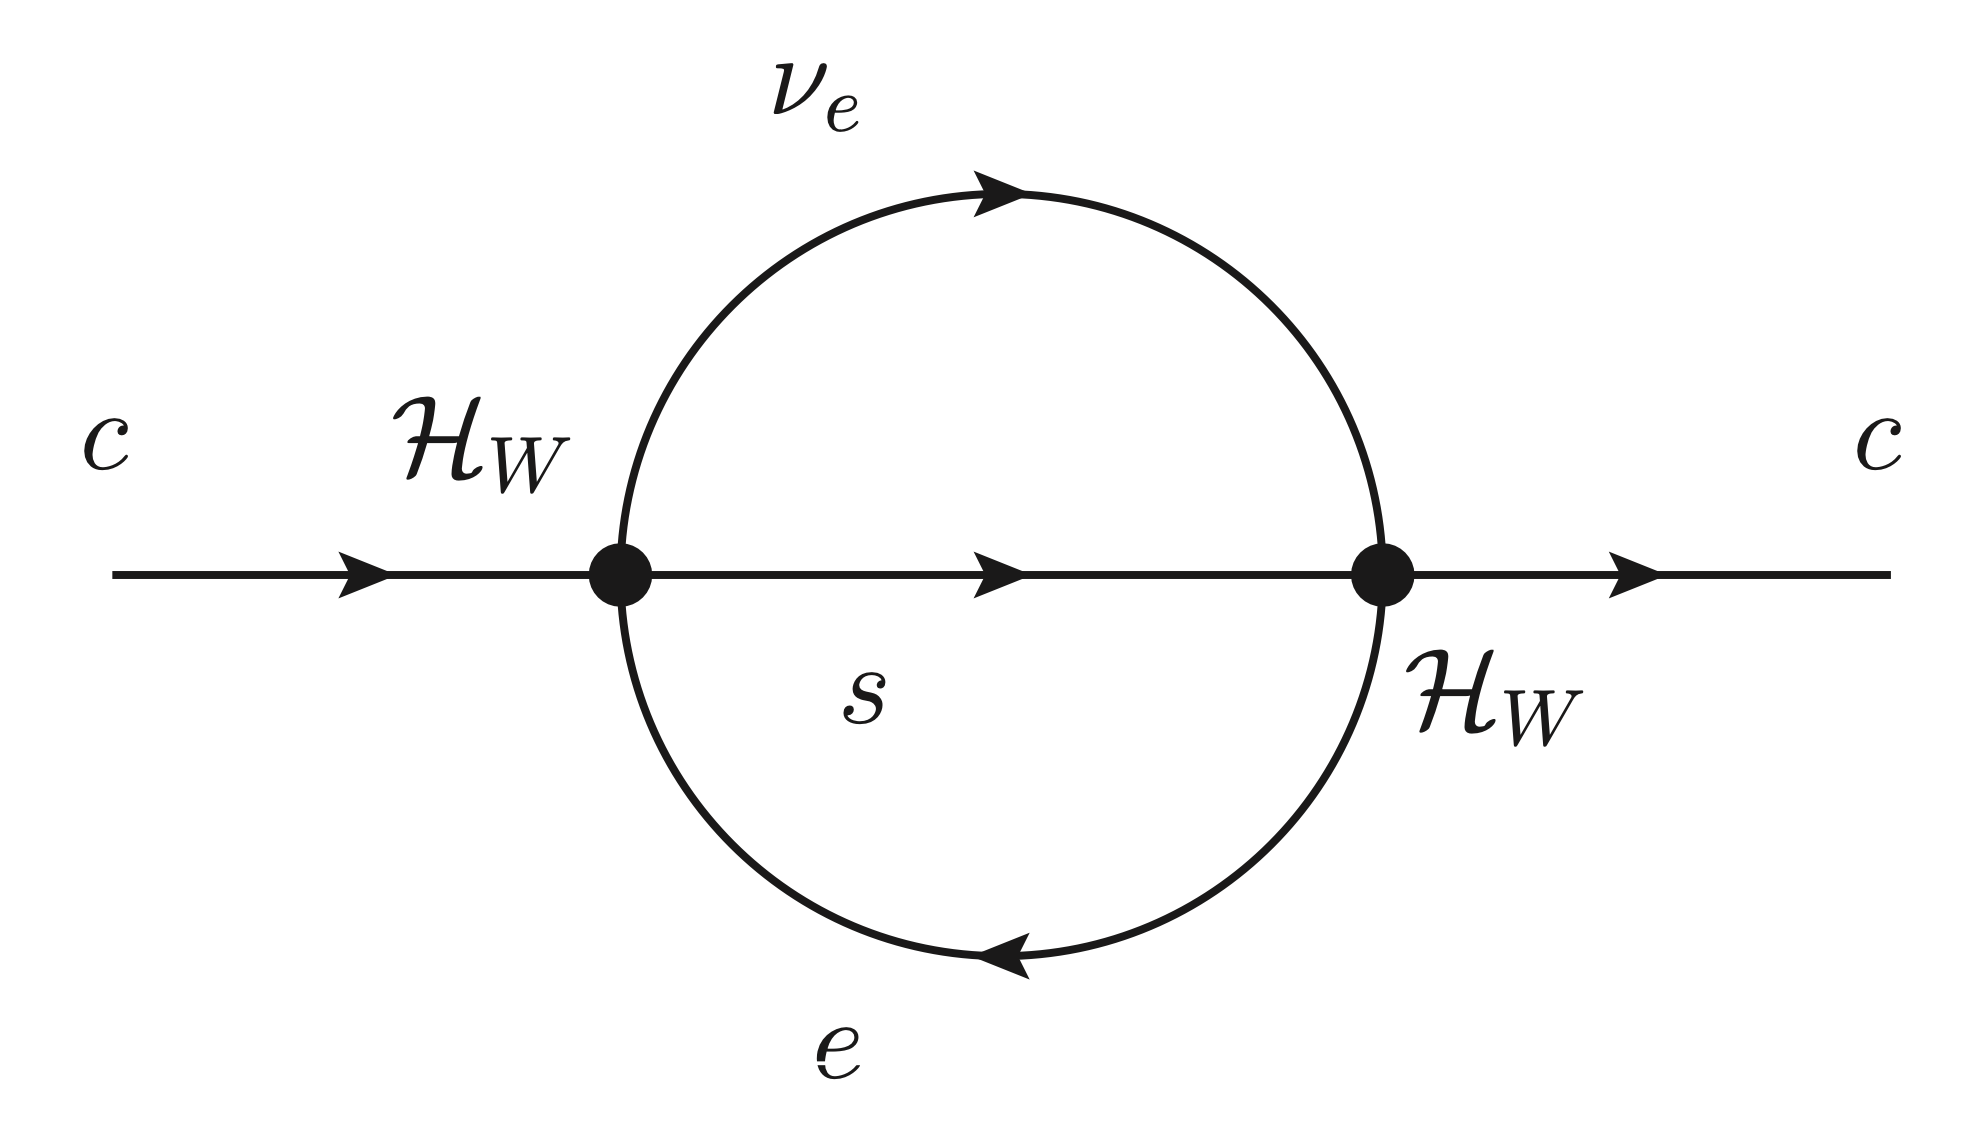
\includegraphics[width=0.4\textwidth]{figures/HQEc.png}
    \caption{算符乘积展开领先幂次贡献\ct{Fael:2019umf}}
    \label{fig:HQEc}
\end{figure}
其衰变宽度为
\begin{equation}
    \Gamma=\frac{1}{\mrm{M}_\mrm{D}} \operatorname{Im}\langle \mrm{D}| i \int \mrm{d}^4 x e^{-i p_\mrm{D} \cdot x} \operatorname{T}\left\{\mathcal{H}_W^{\dagger}(x), \mathcal{H}_W(0)\right\}|\mrm{D}\rangle=\frac{1}{\mrm{M}_\mrm{D}} \operatorname{Im}\langle \mrm{D}| R|\mrm{D}\rangle,
    \label{eq:decaywidth_c}
\end{equation}
其中弱有效哈密顿量为：\begin{equation}
    \mathcal{H}_W=\frac{4 \mrm{G_F}}{\sqrt{2}} \mrm{V_{\mathrm{CKM}}}\left(\mrm{\bar{q}} \gamma_\mrm{L}^\mu \mrm{c}\right)\left(\mrm{\overline{\nu}_{\ell}} \gamma_{\mrm{L} \mu} \mrm{\ell}\right)=\frac{4 \mrm{G_F}}{\sqrt{2}} \mrm{V}_{\mathrm{CKM}} J_\mrm{q}^\mu J_{\mrm{\ell} \mu},
    \end{equation}
其中，$\gamma_{\mathrm{L}}^\mu = \gamma^\mu P_{\mathrm{L}}, \quad P_{\mathrm{L}} = \frac{1 - \gamma_5}{2}$
是左手投影算子，$\mrm{G_{F}}$是费米常数，$\mrm{V}_{\mathrm{CKM}}$是相关的CKM矩阵元模方，$J_\mrm{q}^\mu$ 和 $J_{\mrm{\ell}}^\mu$分别是强子流和轻子流。

式\eqref{eq:decaywidth_c}中的非局域算符的编时乘积可以用一组局域算符展开，
\begin{equation}
    \operatorname{T}\left\{\mathcal{H}_W^{\dagger}(x), \mathcal{H}_W(0)\right\}=\sum C^n(x) \mathscr{O}_n(0).
    \label{eq:OPE}
\end{equation}
其中树图水平上对应的局域算符是两夸克算符，其一般形式为 $\bar{Q}_v\left(i D^{\mu_1} \ldots i D^{\mu_n}\right) Q_v$, $D^{\mu}$是协变微分算子，其本征值为离壳动量$k\sim \Lambda_{\mrm{QCD}}$。 式\eqref{eq:OPE}中,展开系数$C^n(x)$对应于该过程的短程微扰贡献，而受到$1/m_{\mrm{c}}$压低的局域算符矩阵元对应于长程非微扰贡献。前者可以通过微扰理论逐阶计算，后者涉及强相互作用非微扰，需要通过格点量子色动力学或从实验数据中抽取得到。

计算$\mrm{c}\to \mrm{s} e^+\nu$过程分为三步：首先在微扰展开的特定阶，在$\mu\sim m_{\mrm{c}}$处抽取出Wilson系数。由于算符乘积展开是算符之间的关系，可以通过将式\eqref{eq:OPE}置于夸克和胶子态中，计算Wilson系数；其次，Wilson系数必须通过求解对应局域算符的反常量纲并通过重整化群方程演化到$\mu<m_{\mrm{c}}$处；最后，衰变宽度可以用一组局域算符矩阵元（非微扰参数）进行参数化，一般标记为$\mrm{X}_i(\mu)$，
\begin{equation}
    \left.2 M_\mrm{D} \mrm{X}_i(\mu) \equiv\langle \mrm{D}| O_i|\mrm{D}\rangle\right|_\mu.
    \end{equation}
对于D介子半轻单举衰变过程，通常非局域算符通常可以用以下一组局域算符\ct{Fael:2019umf}进行展开\footnote{精确至量纲七算符}，
\begin{equation}
    \begin{array}{ll}
    O_{\mu_3}=\bar{c}_v c_v, & O_{r_G}=\bar{c}_v\left[\left(i D_\mu\right),\left(i D_\nu\right)\right]\left[\left(i D^\mu\right),\left(i D^\nu\right)\right] c_v, \\
    O_{\mu_\pi}=\bar{c}_v(i D)^2 c_v, & O_{r_E}=\bar{c}_v\left[(i v D),\left(i D_\mu\right)\right]\left[(i v D),\left(i D^\mu\right)\right] c_v, \\
    O_{\mu_G}=\bar{c}_v \sigma \cdot G c_v, & O_{s_B}=\bar{c}_v\left[\left(i D_\mu\right),\left(i D_\alpha\right)\right]\left[\left(i D^\mu\right),\left(i D_\beta\right)\right]\left(-i \sigma^{\alpha \beta}\right) c_v, \\
    O_{\rho_D}=\frac{1}{2} \bar{c}_v\left[i D^\mu,\left[i v D, i D_\mu\right]\right] c_v, & O_{s_E}=\bar{c}_v\left[(i v D),\left(i D_\alpha\right)\right]\left[(i v D),\left(i D_\beta\right)\right]\left(-i \sigma^{\alpha \beta}\right) c_v, \\
    O_{\delta \rho_D}=\frac{1}{2} \bar{c}_v\left[i D^\mu,\left[(i D)^2, i D_\mu\right]\right] c_v, & O_{s_{q B}}=\bar{c}_v\left[i D_\mu,\left[i D^\mu,\left[i D_\alpha, i D_\beta\right]\right]\right]\left(-i \sigma^{\alpha \beta}\right) c_v,
    \end{array}
    \end{equation}
其中，$\sigma \cdot G \equiv-i \sigma^{\mu \nu}\left(i D_\mu\right)\left(i D_\nu\right)$，$\sigma^{\mu \nu}=\frac{i}{2}\left[\gamma^\mu, \gamma^\nu\right]$.最终$\mrm{D}\to \mrm{X}_{\mrm{s}}e^{+}\nu$过程的半轻单举衰变宽度用该组局域算符的非微扰矩阵元参数化为
\begin{equation}
    \begin{aligned}
    \frac{\Gamma\left(\mathrm{D} \rightarrow \mathrm{X}_{\mathrm{s}} \ell \nu\right)}{\Gamma_0} & = \left(1 - 8 \rho - 10 \rho^2\right) \mu_3 + (-2 - 8 \rho) \frac{\mu_\mrm{G}^2}{m_\mrm{c}^2} + 6 \frac{\tilde{\rho}_\mrm{D}^3}{m_\mrm{c}^3} \\
    & + \frac{16}{9} \frac{r_\mrm{G}^4}{m_\mrm{c}^4} + \frac{32}{9} \frac{r_\mrm{E}^4}{m_\mrm{c}^4} - \frac{34}{3} \frac{s_\mrm{B}^4}{m_\mrm{c}^4} + \frac{74}{9} \frac{s_\mrm{E}^4}{m_\mrm{c}^4} + \frac{47}{36} \frac{s_{\mathrm{qB}}^4}{m_\mrm{c}^4} + \frac{\tau_0}{m_\mrm{c}^3},
    \end{aligned}
\end{equation}
%其中，$\rho=m_s^2 / m_c^2$, $\Gamma_{0}=\frac{G_F^2m_{c}^5|V_{cs}|^2}{192\pi^3}$。

本文将讨论D介子半轻单举衰变过程中的物理可观测量的构造，其依赖于这些局域算符的非微扰强子矩阵元；与此同时，从实验数据中抽取出相应物理可观测量的实验观测值，与理论表达式一起进行全局拟合以期实现对局域算符非微扰强子矩阵元的拟合抽取；D介子半轻衰变与非轻衰变的不同之处仅在于其Wilson系数不同，因此本文关于局域算符非微扰强子矩阵元的拟合估计值可直接用于D介子衰变宽度的理论计算。

\section{本章回顾}
本章对粒子物理标准模型和量子色动力学进行简单介绍，此外，对量子色动力学的两种近似对称性（手征对称性和重夸克对称性）进行讨论，基于重夸克对称性，讨论了重夸克有效理论和基于重夸克有效理论的算符乘积展开，最终衰变宽度可以用一组局域算符的非微扰矩阵元进行参数化。这是本文对D介子进行系统性研究的理论基础。

\chapter{粲介子半轻单举衰变的理论研究}
本章从幂次修正和微扰修正两方面介绍本研究的相关工作：对于幂次修正，本文详细讨论了树图水平上量纲三与量纲五算符对应Wilson系数的匹配与相空间解析积分。对于微扰修正，本文讨论了单圈水平上领先幂次修正的解析积分，并给出电子能谱的解析形式。此外简单介绍了高量纲算符的参数化方案。
\section{幂次修正}
\subsection{B介子半轻单举衰变}
本节以$\mrm{b \to c}$和$\mrm{b \to u}$过程为例，讨论树图水平上量纲三与量纲五算符对应Wilson系数匹配和相空间解积分，可得$\mrm{b\to c}$和$\mrm{b\to u}$衰变过程的电子能谱和衰变宽度。

$\mrm{b \rightarrow c \ell \nu}$过程的弱有效哈密顿为\ct{manohar2000heavy}
\begin{equation}
    \mathcal{H}_W=\frac{4 \mrm{G_F}}{\sqrt{2}} \mrm{V}_{\mathrm{CKM}}\left(\bar{q} \gamma_\mrm{L}^\mu\mrm{c}\right)\left(\bar{\nu}_{\ell} \gamma_{\mrm{L} \mu} \ell\right)=\mrm{\frac{4 G_F}{\sqrt{2}} V_{\mathrm{CKM}} }J_\mrm{q}^\mu J_{\mrm{\ell} \mu},
    \end{equation}
其中, $\gamma_\mrm{L}^\mu=\gamma^\mu P_\mrm{L}, P_\mrm{L}=\left(1-\gamma_5\right) / 2$ 是左手投影算符, $\mrm{G_F}$ 是费米常数, $\mrm{V}_{\mathrm{CKM}}$是相关的Cabibbo-Kobayashi-Maskawa（CKM）矩阵元模方, $J_\mrm{q}^\mu$ and $J_{\mrm{\ell}}^\mu$ 分别是强子和轻子流。基于洛伦兹对称性和宇称-电荷共轭对称性，强子流对应振幅模方\footnote{轻子流对应振幅模方是$ L^{\alpha \beta}=2\left(p_\mrm{e}^\alpha p_{\mrm{v_e}}^\beta+p_\mrm{e}^\beta p_{\mrm{v_e}}^\alpha-g^{\alpha \beta} p_\mrm{e} \cdot p_{\mrm{v_e}}-i \epsilon^{\eta \beta \lambda \alpha} p_{\mrm{e} \eta} p_{\mrm{v_e} \lambda}\right)$}可以用一组基底进行展开，
\begin{equation}
        W_{\alpha \beta}=-g_{\alpha \beta} W_1+v_\alpha v_\beta W_2-i \epsilon_{\alpha \beta \mu \nu} v^\mu q^\nu W_3+q_\alpha q_\beta W_4+\left(v_\alpha q_\beta+v_\beta q_\alpha\right) W_5,
\end{equation}
其中, $p_{\mrm{\nu_{e}}}$, $p_{\mrm{e}}$, $v$, $q$分别是反电子中微子，电子，轻子对的动量和$\mrm{\bar{B}}$介子速度。 $W_{j}\text{是}q^{2}\text{和}v\cdot q$的实函数\footnote{计算$W_{j}(q^{2},v\cdot q)$关于$v\cdot q$的积分时，需将$W_{j}(q^{2},v\cdot q)$解析延拓到$v\cdot q$复平面，对应地复变函数是$T_{j}(q^{2},v\cdot q)$}。

强子张量定义如下, 
\begin{equation}
    W_{\alpha \beta}=\sum_{\mrm{X_c}}(2 \pi)^3 \delta^4\left(p_B-q-p_{\mrm{X_c}}\right) \frac{1}{2m_\mrm{B}} \times\left\langle\mrm{\bar{B}\left(p_B\right)}\right| J_{\mrm{L} \alpha}^{\dagger}\left|\mrm{X_c}\left(p_{\mrm{X_c}}\right)\right\rangle\left\langle\mrm{X_c}\left(p_{\mrm{X_c}}\right)\right| J_{\mrm{L} \beta}\left|\mrm{\bar{B}\left(p_B\right)}\right\rangle.
    \end{equation}
将强子张量和轻子张量进行洛伦兹指标缩并并经过适当的相空间积分，$\mrm{\bar{B}}$介子半轻单举衰变宽度为：
\begin{equation}
    \begin{aligned}
    & \frac{\mrm{d} \Gamma}{\mrm{d} q^2 \mrm{d} E_{\mathrm{\bar{\nu}_e}} \mrm{d} E_{\mathrm{e}}} \\
    = & \frac{\mrm{G_F^2} \mrm{\left| V_{\mathrm{cb}} \right|^2} m_{\mathrm{b}}^5}{2 \pi^3} \left[ W_1 q^2 + W_2 \left( 2 E_{\mathrm{e}} E_{\overline{v}_e} - q^2 / 2 \right) + W_3 q^2 \left( E_{\mathrm{e}} - E_{\tilde{v}_e} \right) \right] \theta \left( 4 E_{\mathrm{e}} E_{\overline{v}_e} - q^2 \right).
    \end{aligned}
\end{equation}

其中，$W_{i}, i=1,2,3$是$\mrm{\bar{B}}$介子的标量结构函数。通过完整理论和有效理论之间对$W_{i}$进行匹配可得Wilson系数，随后对运动学变量进行解析积分可得$\mrm{\bar{B}}$介子半轻单举衰变过程的电子能谱，衰变宽度和各种物理观测量。

在微扰论领头阶，考虑强子流的编时乘积
\begin{equation}
    T_{\alpha \beta} = -\mathrm{i} \int \mrm{d}^4 x \, e^{-\mathrm{i} q \cdot x} \frac{\left\langle \mrm{\bar{B}} \left( {\mathrm{p_B}} \right) \right| \operatorname{T} \left[ J_{\mrm{L} \alpha}^{\dagger} (x) J_{\mrm{L}\beta} (0) \right] \left| \mrm{\bar{B}} \left( \mathrm{p_{B}} \right) \right\rangle}{2 m_{\mathrm{B}}}.
\end{equation}

在流的编时乘积中插入一组完备正交末态集$\mrm{\sum\ket{X}\bra{X}}$, 强子流\footnote{在夸克层次上，$J_{\mrm{L} \beta}(0)\ket{\mrm{\bar{B}}}=\mrm{\bar{c}} \gamma_\beta P_\mrm{L} \mrm{b\ket{\bar{B}}}$表示湮灭初态b夸克，产生末态c夸克；$J_{\mrm{L} \alpha}^{\dagger}(0)\mrm{\ket{\bar{B}}}=\mrm{\bar{b}}\gamma_{\alpha}P_{\mrm{R}}\mrm{c\ket{\bar{B}}}$对应于产生$\mrm{\bar{c}}$夸克和两个b夸克（多粒子直积态）,这些态和完备末态集进行投影，挑选出$\mrm{X_{c}}$和$\mrm{X_{b\bar{b}c}}$}
    跃迁至两个个末态\footnote{$X_{bb\bar{c}}$被能量守恒定律所禁戒。}，分别是$X_{c}$和$X_{bb\bar{c}}$。以$X_{c}$为例，这里的投影指的是$\bra{X}c\rangle=\bra{X_{c}}$, 类似地, $\bra{X}bb\bar{c}\rangle=\bra{X_{bb\bar{c}}}$。
    基于Heavside-Theta函数的积分表示\footnote{$\theta\left(x^0\right)=-\frac{1}{2 \pi i} \int_{-\infty}^{\infty} d \omega \frac{e^{-i \omega x^0}}{\omega+i \varepsilon}$}，并结合场的平移算符，对$x$和$\omega$进行积分可得：
    \begin{equation}
        T_{\alpha \beta}=\sum_{X_c} \frac{\langle\bar{B}| J_{L \alpha}^{\dagger}\left|X_c\right\rangle\left\langle X_c\right| J_{L \beta}|\bar{B}\rangle}{2 m_B\left(m_B-E_X-q^0+i \varepsilon\right)}(2 \pi)^3 \delta^3\left(\mathbf{q}+\mathbf{p}_X\right).
        \label{eq:T_ab}
    \end{equation}
类似的，式\eqref{eq:T_ab}同样可以用一组基底进行展开，
\begin{equation}
    T_{\alpha \beta}=-g_{\alpha \beta} T_1+v_\alpha v_\beta T_2-i \varepsilon_{\alpha \beta \mu \nu} \nu^\mu q^v T_3+q_\alpha q_\beta T_4+\left(v_\alpha q_\beta+v_\beta q_\alpha\right) T_5.
    \end{equation}
基于算符乘积展开，当$x\sim 0$时该非局域流算符的编时乘积在可以用一组局域算符进行级数展开，即
\begin{equation}
    \operatorname{T}[J_{\mrm{L} \alpha}^{\dagger}(x) J_{\mrm{L} \beta}(0)]=\sum C^n(x) \mathscr{O}_n(0),
\end{equation}
其中Wilson系数可以通过量子场论微扰论进行逐阶微扰展开。从QCD费曼规则出发，强子流编时乘积在微扰论的领头阶有：
\begin{equation}
    \bar{u} \frac{1}{\left(m_{\mathrm{b}} v - q + k\right)^2 - m_{\mathrm{c}}^2 + i \varepsilon} \gamma_{\alpha} P_{\mathrm{L}} \left(m_{\mathrm{b}} \slashed{p} - \slashed{q} + \slashed{k}\right) \gamma_{\beta} P_{\mathrm{L}} u,
\end{equation}
其中，$m_{\mrm{b}}, m_{\mrm{c}}$是底夸克和粲夸克质量，$k$是底夸克的离壳动量（$k\sim \Lambda_{\mrm{QCD}}$）。对$\frac{k}{m_{\mrm{b}}}$在零附近进行泰勒展开，领先幂次的结果是
\begin{equation}
    \begin{aligned}
    & \frac{1}{\Delta_0} \bar{u}\left[\left(m_{\mathrm{b}} v - q\right)_{\alpha} \gamma_{\beta} + \left(m_{\mathrm{b}} v - q\right)_{\beta} \gamma_{\alpha} - \left(m_{\mathrm{b}} \slashed{v} - \slashed{q}\right) g_{\alpha \beta}\right. \\
    & \left.\quad -i \epsilon_{\alpha \beta \lambda \eta} \left(m_{\mathrm{b}} v - q\right)^{\lambda} \gamma^{\eta} \right] P_{\mathrm{L}} u,
    \end{aligned}
\end{equation}
    其中，$\Delta_0 = \left( m_{\mathrm{b}} v - q \right)^2 - m_{\mathrm{c}}^2 + i \varepsilon$
。底夸克之间的量纲三算符包括$\mrm{\bar{b}}\gamma^{\mu}\mrm{b}$和$\mrm{\bar{b}}\gamma^{\mu}\gamma^{5}\mrm{b}$, 前者的零分量对应底夸克数算符，后者的贡献由于强相互作用中宇称守恒所禁戒。此外领先幂次的水平上有效粲夸克场和完整粲夸克场之间仅存在一个指数形式因子的差别，没有$1/m_{\mrm{b}}$的幂次修正。
\begin{equation}
    T_{\mathrm{\alpha \beta}}^0 = \left( -g_{\alpha \beta} \right) \left( m_{\mathrm{b}} - q \cdot v \right) \frac{1}{2 \Delta_0} + v_{\alpha} v_{\beta} \frac{m_{\mathrm{b}}}{\Delta_0} - i \varepsilon_{\alpha \beta \lambda \eta} v^{\lambda} q^{\eta} \frac{1}{2 \Delta_0} + \ldots.,
\end{equation}
与$T_{\alpha\beta}$的一般形式进行匹配可得：
\begin{equation}
    T_1^{(0)} = \frac{1}{2 \Delta_0} \left( m_{\mathrm{b}} - q \cdot v \right) \quad T_2^{(0)} = \frac{1}{\Delta_0} m_{\mathrm{b}} \quad T_3^{(0)} = \frac{1}{2 \Delta_0}.
\end{equation}
某个衰变过程的衰变宽度与其向前散射振幅的虚部相关，$-\frac{1}{\pi} \operatorname{Im} \operatorname{T}_j=W_j$ (仅考虑左手割线)。利用\footnote{其中P指的是主值。}
\begin{equation}
    \frac{1}{\omega+i \varepsilon}=P \frac{1}{\omega}-i \pi \delta(\omega),
    \end{equation}
可得：
\begin{equation}
    \begin{aligned}
    & W_1^{(0)} = \frac{1}{4} \left( 1 - \frac{q \cdot v}{m_{\mathrm{b}}} \right) \delta\left[ v \cdot q - \left( \frac{q^2 + m_{\mathrm{b}}^2 - m_{\mathrm{c}}^2}{2 m_{\mathrm{b}}} \right) \right], \\
    & W_2^{(0)} = \frac{1}{2} \delta\left[ v \cdot q - \left( \frac{q^2 + m_{\mathrm{b}}^2 - m_{\mathrm{c}}^2}{2 m_{\mathrm{b}}} \right) \right], \\
    & W_3^{(0)} = \frac{1}{4 m_{\mathrm{b}}} \delta\left[ v \cdot q - \left( \frac{q^2 + m_{\mathrm{b}}^2 - m_{\mathrm{c}}^2}{2 m_{\mathrm{b}}} \right) \right].
    \end{aligned}
\end{equation}

次领先幂次的结果为：
\begin{equation}
    \begin{aligned}
    & \frac{1}{\Delta_0} \bar{u}\left(k_\alpha \gamma_\beta+k_\beta \gamma_\alpha-g_{\alpha \beta} \slashed{k}-i \epsilon_{\alpha \beta \lambda \eta} k^\lambda \gamma^\eta\right) P_{\mathrm{L}} u \\
    & \quad-\frac{2 k \cdot\left(m_{\mathrm{b}} v-q\right)}{\Delta_0^2} \bar{u}\left[\left(m_{\mathrm{b}} v-q\right)_\alpha \gamma_\beta+\left(m_{\mathrm{b}} v-q\right)_\beta \gamma_\alpha\right. \\
    & \left.\quad-\left(m_{\mathrm{b}} \slashed{v}-\slashed{q}\right) g_{\alpha \beta}-i \epsilon_{\alpha \beta \lambda \eta}\left(m_{\mathrm{b}} v-q\right)^\lambda \gamma^\eta\right] P_{\mathrm{L}} u .
    \end{aligned}
    \label{eq:k_linear}
\end{equation}
式\eqref{eq:k_linear}中出现新算符是$\mrm{\bar{b}}(\gamma_\lambda i D_\tau -m_{\mrm{b}}v_{\tau})\mrm{b}$和$\mrm{\bar{b}}(\gamma_\lambda \gamma_5 i D_\tau -m_{\mrm{b}}v_{\tau})\mrm{b}$，在粲夸克场做$1/m_{\mrm{b}}$展开的领先幂次水平上，这两个算符最终是$\mrm{\bar{b_{v}}} \gamma_\lambda i D_\tau\mrm{ b_{v}}$和$\mrm{\bar{b_{v}}}\gamma_\lambda \gamma_5 i D_\tau\mrm{b_{v}}$,对于前者，由于重夸克有效理论中重夸克场幂次展开的领头阶拉格朗日方程$i v\cdot D=0$的约束，其贡献被禁戒；对于后者，由于强相互作用中电荷宇称守恒的约束，其贡献也为0(量纲四算符的非微扰矩阵元贡献为0)。


量纲五算符存在三个来源。首先次领先幂次的结果中若重夸克场幂次展开到线性项，则会包含量纲五算符的贡献; 其次，次次领先幂次的修正同样会包含量纲五算符的贡献；最后，由于粲夸克之间色磁算符对应矩阵元的量纲为五，因此在树图水平上讨论单胶子发射图对量纲五算符修正的贡献是必要的\footnote{在树图水平上，存在一种收缩方式使得色磁算符矩阵元贡献非零，即单胶子发射}。

考虑底夸克场的幂次展开，
\begin{equation}
   \mrm{b(x)}=e^{-i m_\mrm{b} v \cdot x}\left(1+\frac{i \slashed{D}}{2 m_\mrm{b}}\right)\mrm{ b_v(x)},
    \end{equation}
对应拉格朗日量的幂次修正项为：
\begin{equation}
    \mathcal{L}_1=-\mrm{\bar{b}_v} \frac{D^2}{2 m_\mrm{b}} \mrm{b_v}-\mrm{\bar{b}_v} g \frac{G_{\alpha \beta} \sigma^{\alpha \beta}}{4 m_\mrm{b}}\mrm{b_v}.
    \end{equation}
以$\mrm{\bar{b}} \gamma_\lambda\left(i D_\tau-m_b v_\tau\right)\mrm{b}$为例，其在微扰论意义上的完整形式是：
    \begin{equation}
        \begin{aligned}
            \{\mrm{\bar{b}} \gamma_\lambda\left(i D_\tau-m_\mrm{b} v_\tau\right) b\} e^{\int \mathcal{L}_1  \mrm{d}^4 x}&=\mrm{\bar{b}_v} \gamma_\lambda i D_\tau b_v+i \int \mrm{d}^4 x \operatorname{T}\left[\mrm{\bar{b}_v}\gamma_\lambda i D_\tau\mrm{b_v(0)} \mathcal{L}_1(x)\right]\\
            &+\mrm{\bar{b}}_v\left(\frac{-i\slashed{D}}{2 m_\mrm{b}}\right) \gamma_\lambda i D_\tau \mrm{b_v}+\mrm{\bar{b}_v} \gamma_\lambda i D_\tau \frac{i \slashed{D}}{2 m_\mrm{b}} \mrm{b_v} +\cdots,\\
        \end{aligned}
    \label{eq:k_linear_expand}
        \end{equation}
式\eqref{eq:k_linear_expand}的左边是底夸克场之间流算符，右边第二项表示了重夸克有效理论拉格朗日量的次领先幂次对该流算符的修正。右边的其余部分是底夸克场幂次展开到线性项所引入的修正。

重夸克有效理论中的传播子方程为$iv\cdot D S_{h}(x-y)=\delta(x-y)$，最终可以基于非微扰参数$\lambda_1$和$\lambda_2$参数化式\eqref{eq:k_linear}，其中
\begin{equation}
    \begin{aligned}
    2 \lambda_1 & =-\left\langle \mrm{\bar{B}}\right| \bar{Q}_{\mrm{v_r}} D_{\perp}^2 Q_{\mrm{v_r}}\left|\mrm{\bar{B}}\right\rangle, \\
    16\left(\mathbf{S}_\mrm{b} \cdot \mathbf{S}_{\mrm{\ell}}\right) \lambda_2\left(m_\mrm{c}\right) & =\left\langle \mrm{\bar{B}}\right| \bar{Q}_{\mrm{v_r}} g \sigma_{\alpha \beta} G^{\alpha \beta} Q_{\mrm{v_r}}\left|\mrm{\bar{B}}\right\rangle .
    \end{aligned}
    \end{equation}
其中$\ket{\mrm{\bar{B}}}$是渐进HQET态，$\bar{Q}_{\mrm{v_r}}$是有效重夸克场，$\mathbf{S}_\mrm{b}$和$\mathbf{S}_{\mrm{\ell}}$分别是$\mrm{\bar{B}}$介子中底夸克和轻夸克的自旋矢量。
整理结果可得：
\begin{equation}
    \begin{aligned}
    & T_1^{(1)}=-\frac{1}{2 m_b}\left(\lambda_1+3 \lambda_2\right)\left\{\frac{1}{6 \Delta_0}-\frac{\left(m_b-q \cdot v\right)^2}{\Delta_0^2}+\frac{2}{3} \frac{\left[q^2-(q \cdot v)^2\right]}{\Delta_0^2}\right\}, \\
    & T_2^{(1)}=-\frac{1}{2 m_b}\left(\lambda_1+3 \lambda_2\right)\left[\frac{5}{3 \Delta_0}-\frac{2 m_b\left(m_b-v \cdot q\right)}{\Delta_0^2}+\frac{4}{3} \frac{m_b v \cdot q}{\Delta_0^2}\right], \\
    & T_3^{(1)}=\frac{1}{2 m_b}\left(\lambda_1+3 \lambda_2\right) \frac{5}{3}\left(\frac{m_b-v \cdot q}{\Delta_0^2}\right) .
    \end{aligned}
    \end{equation}

考虑次次领先幂次的结果，
\begin{equation}
    \begin{aligned}
    -2 & \frac{k \cdot\left(m_{\mathrm{b}} v-q\right)}{\Delta_0^2} \bar{u}\left(k_\alpha \gamma_\beta+k_\beta \gamma_\alpha-g_{\alpha \beta}\slashed{k}-i \epsilon_{\alpha \beta \lambda \eta} k^\lambda \gamma^\eta\right) P_{\mathrm{L}} u \\
    & +\left\{\frac{4\left[k \cdot\left(m_{\mathrm{b}} v-q\right)\right]^2}{\Delta_0^3}-\frac{k^2}{\Delta_0^2}\right\} \bar{u}\left[\left(m_{\mathrm{b}} v-q\right)_\alpha \gamma_\beta+\left(m_{\mathrm{b}} v-q\right)_\beta \gamma_\alpha\right. \\
    & \left.-\left(m_{\mathrm{b}} \slashed{v}-\slashed{q}\right) g_{\alpha \beta}-i \epsilon_{\alpha \beta \lambda \eta}\left(m_{\mathrm{b}} v-q\right)^\lambda \gamma^\eta\right] P_{\mathrm{L}} u .
    \end{aligned}
\end{equation}
新出现算符包括:
$$\bar{b} \gamma^\lambda \left(i D-m_b v\right)^{(\alpha}\left(i D-m_b v\right)^{\beta)} b,$$
$$\bar{b} \gamma^\lambda \gamma_5\left(i D-m_b v\right)^{(\alpha}\left(i D-m_b v\right)^{\beta)} b.$$

前者可以被$\lambda_1$参数化而后者贡献由于强相互作用中宇称守恒所禁戒。
整理可得：
\begin{equation}
    \begin{aligned}
    & T_1^{(2)}=\frac{1}{6} \lambda_1\left(m_{\mathrm{b}}-v \cdot q\right)\left\{\frac{4}{\Delta_0^3}\left[q^2-(v \cdot q)^2\right]-\frac{3}{\Delta_0^2}\right\}, \\
    & T_2^{(2)}=\frac{1}{3} \lambda_1 m_{\mathrm{b}}\left\{\frac{4}{\Delta_0^3}\left[q^2-(v \cdot q)^2\right]-\frac{3}{\Delta_0^2}-\frac{2 v \cdot q}{m_{\mathrm{b}} \Delta_0^2}\right\}, \\
    & T_3^{(2)}=\frac{1}{6} \lambda_1\left\{\frac{4}{\Delta_0^3}\left[q^2-(v \cdot q)^2\right]-\frac{5}{\Delta_0^2}\right\}.
    \end{aligned}
\end{equation}
此外，对来源于$ \mathcal{L}_1$修正的单胶子发射图，以胶子动量$p$为展开参数，$p$的线性项贡献可以被$\lambda_{2}$参数化，可得：
\begin{equation}
     T_1^{(g)}=\lambda_2 \frac{\left(m_\mrm{b}-v \cdot q\right)}{2 \Delta_0^2},\quad
     T_2^{(g)}=-\lambda_2 \frac{m_\mrm{b}}{\Delta_0^2}, \quad
     T_3^{(g)}=\lambda_2 \frac{1}{2 \Delta_0^2}.
    \end{equation}
树图水平上量纲五算符对应的结构函数包括:
$$
T_j=T_j^{(1)}+T_j^{(2)}+T_j^{(g)}.
$$
微分衰变宽度中的$W_{i}$是$T_{i}$的虚部，基于$$
-\frac{1}{\pi} \operatorname{Im}\left(\frac{1}{\Delta_0}\right)^{n+1}=\frac{(-1)^n}{n!} \delta^{(n)}\left[\left(m_\mrm{b} v-q\right)^2-m_\mrm{c}^2\right].
$$
可得树图水平上量纲三算符和量纲五算符非微扰矩阵元对应的Wilson系数，这是本文对相空间积分以得到电子能谱和物理可观测量的基础。

\subsubsection{运动学分析}
从树图阶的三微分衰变宽度出发，经过两重解析积分可得电子能谱的理论结果。
\paragraph{1. 中微子能量的积分区域}

在初态底夸克质心系中(z轴正方向是虚$W^{*}$的飞行方向)，中微子能量的表达式是$$E_\nu=\frac{q^2}{2E_\mrm{e}(1-\cos{\theta})},$$其中$\theta$是中微子与电子动量方向的夹角，中微子积分区域的下限是$q^{2}/(4E_\mrm{e})$,对应电子和电子中微子反向飞行\footnote{背对背飞行并不意味着$\vec{p_{\mrm{e}}}+\vec{P_{\mrm{\nu}}}=0$。事实上，忽略电子质量并结合电子在壳条件，$|\vec{p_{\mrm{e}}}|=E_{\mrm{e}}$并非$|\vec{p_{\mrm{e_{z}}}}|=E_{\mrm{e}}$.}($\theta=\pi$)。 
物理区域的上限由末态强子$\mrm{H_{\mrm{c}}}$在壳条件决定,即$\frac{m_{\mathrm{B}}^2 + q^2 - m_{\mathrm{D}}^2}{2 m_{\mathrm{B}}} - E_{\mathrm{e}}$，
\begin{equation}
    \int_{\frac{q^2}{4 E_{\mathrm{e}}}}^{\frac{m_{\mathrm{B}}^2 + q^2 - m_{\mathrm{D}}^2}{2 m_{\mathrm{B}}} - E_{\mathrm{e}}} \frac{\mathrm{d} \Gamma}{\mathrm{d} q^2 \, \mathrm{d} E_{\mathrm{e}} \, \mathrm{d} E_{\mathrm{\nu_e}}} \, \mathrm{d} E_{\mathrm{\nu_e}}
    = \int_{-\infty}^{\infty} \frac{\mathrm{d} \Gamma}{\mathrm{d} q^2 \, \mathrm{d} E_{\mathrm{e}} \, \mathrm{d} E_{\mathrm{\nu_e}}} \theta(4 E_{\mathrm{e}} E_{\mathrm{\nu_e}} - q^2) \, \mathrm{d} E_{\mathrm{\nu_e}}.
    \label{eq:2:36}
\end{equation}
式\eqref{eq:2:36}等号右侧被积函数的完整形式是
\begin{equation}
    \frac{\mathrm{d} \Gamma}{\mathrm{d} q^2 \, \mathrm{d} E_{\mathrm{e}} \, \mathrm{d} E_{\mathrm{\nu_e}}} \theta(4 E_{\mathrm{e}} E_{\mathrm{\nu_e}} - q^2) \theta\left(\frac{m_{\mathrm{B}}^2 + q^2 - m_{\mathrm{D}}^2}{2 m_{\mathrm{B}}} - E_{\mathrm{e}} - E_{\mathrm{\nu_e}}\right),
\end{equation}
如图\ref{fig:2.2}所示，绿色曲面是$E_\mrm{\nu}$的积分下限，蓝色曲面是$E_\mrm{\nu}$的积分上限，橙色曲面是粲夸克传播子给出的狄拉克$\delta$函数对中微子能量的约束。这里$m_{\mrm{b}}=4.18\GeV,m_{\mrm{c}}=1.27\GeV,m_{\mrm{\bar{B}}}=5.28\GeV,m_{\mrm{D}}=1.86\GeV$。粲夸克传播子给出的狄拉克$\delta$函数对中微子能量的约束曲面位于中微子能量的物理区域以内。因此第二个 Heavside-Theta 函数天然满足\footnote{物理区域的上限并非实际积分上限（实际的积分上限由Heavside-Theta函数给出），两者的差别反映了强子和夸克之间的差异。}。
\begin{figure}[h]
    \centering 
    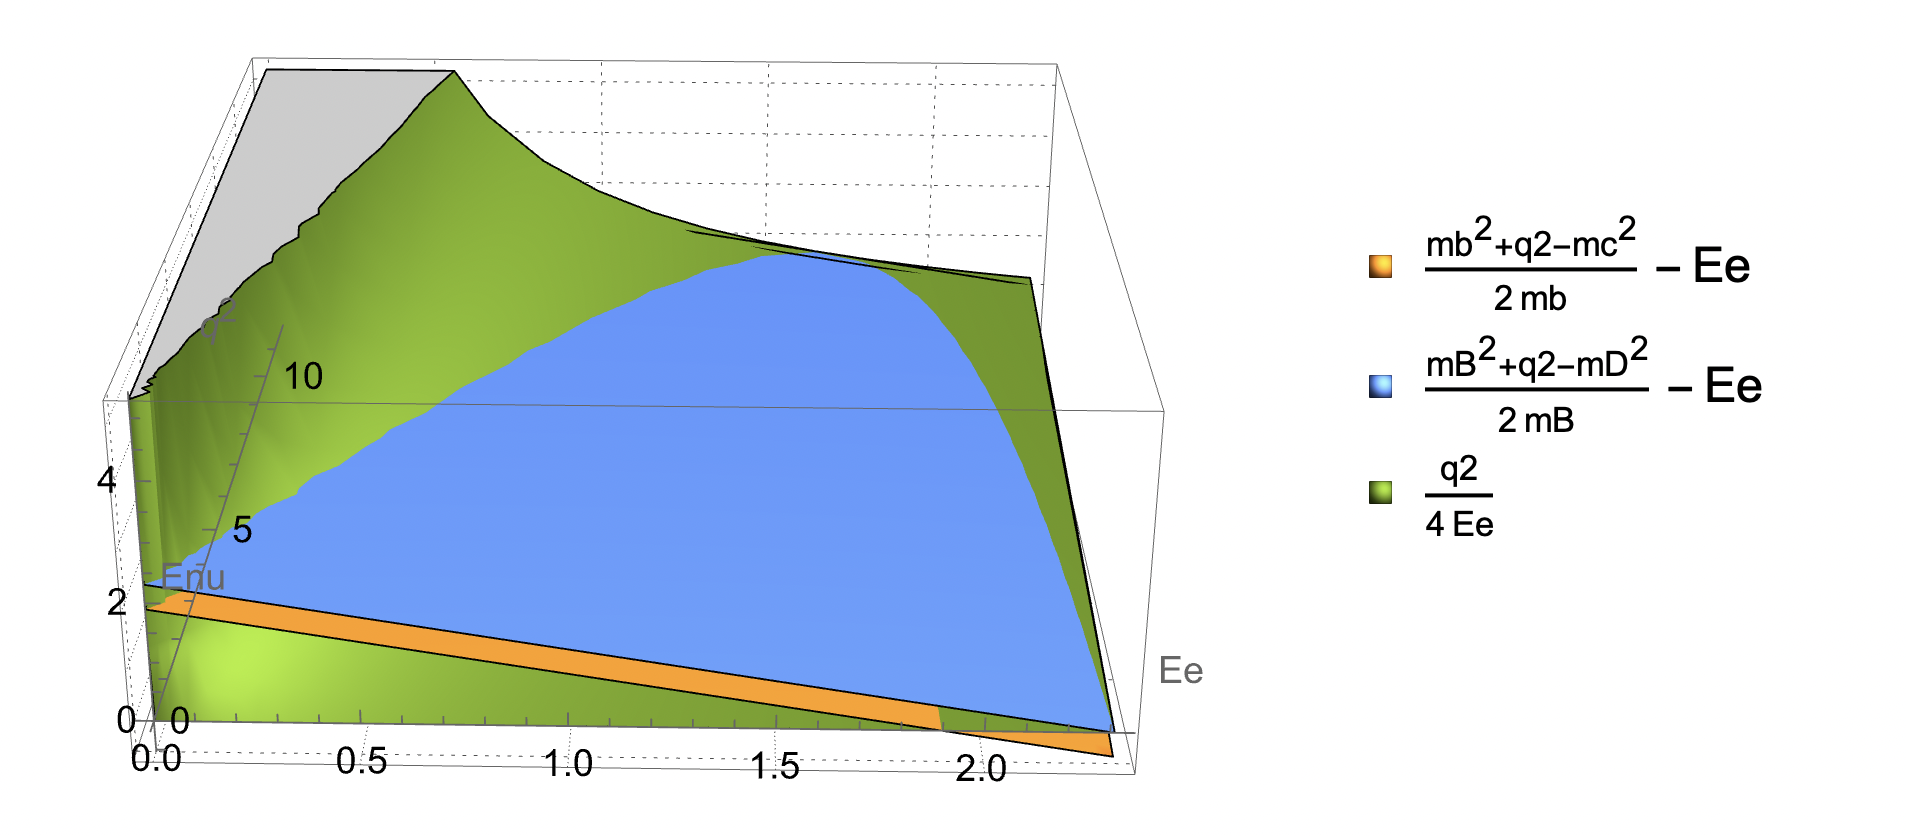
\includegraphics[width=0.8\textwidth]{figures/treephase3.png}
    \caption{中微子能量积分区域}
    \label{fig:2.2}
    \end{figure}

完成$E_\mrm{\nu}$积分后，整体留下Heavside-Theta 函数为：
\begin{equation}
    \theta(4 E_{\mathrm{e}} E_{\mrm{\nu_{e}}} - q^2) \rightarrow \theta\left(\frac{m_{\mathrm{b}}^2 + q^2 - m_{\mathrm{c}}^2}{2 m_{\mathrm{b}}} - E_{\mathrm{e}} - \frac{q^2}{4 E_{\mathrm{e}}}\right).
\end{equation}
将Heavside-Theta 函数无量纲化，可得双微分衰变宽度如下：
\begin{equation}
    \begin{aligned}
    \frac{\mathrm{d} \Gamma}{\mathrm{d} \hat{q}^2 \, \mathrm{d} y} = & \frac{\mrm{G_F^2}m_{\mathrm{c}}^5 \left| \mrm{V_{\mathrm{cb}}} \right|^2}{192 \pi^3}\left\{ \theta ( z ) \left[ 12 \left( y - \hat{q}^2 \right) \left( 1 + \hat{q}^2 - \rho - y \right) \right. \right. \\
    & - \frac{2 \lambda_1}{m_{\mathrm{c}}^2} \left( 4 \hat{q}^2 - 4 \hat{q}^2 \rho + 4 \hat{q}^4 - 3 y + 3 \rho y - 6 \hat{q}^2 y \right) \\
    & \left. - \frac{6 \lambda_2}{m_{\mathrm{c}}^2} \left( - 2 \hat{q}^2 - 10 \hat{q}^2 \rho + 10 \hat{q}^4 - y + 5 \rho y - 10 \hat{q}^2 y \right) \right] \\
    & + \frac{\delta(z)}{y^2} \left[ - \frac{2 \lambda_1}{m_{\mathrm{c}}^2} \left( 2 \hat{q}^6 + \hat{q}^4 y^2 - 3 \hat{q}^2 y^3 - \hat{q}^2 y^4 + y^5 \right) \right. \\
    & \left. - \frac{6 \lambda_2}{m_{\mathrm{c}}^2} \hat{q}^2 \left( \hat{q}^2 - y \right) \left( 5 \hat{q}^2 - 8 y + y^2 \right) \right] \\
    & \left. + \frac{\delta^{\prime}(z)}{y^3} \left[ - \frac{2 \lambda_1}{m_{\mathrm{c}}^2} \hat{q}^2 \left( y^2 - \hat{q}^2 \right)^2 \left( y - \hat{q}^2 \right) \right] \right\},
    \end{aligned}
    \end{equation}
其中，$y = \frac{2 E_{\mathrm{e}}}{m_{\mathrm{b}}}, \quad \hat{q}^2 = \frac{q^2}{m_{\mathrm{b}}^2}, \quad \rho = \frac{m_{\mathrm{c}}^2}{m_{\mathrm{b}}^2}\quad z=1+\hat{q}^2-\rho-\hat{q}^2 / y-y$ 。
\paragraph{2. 轻子对不变质量平方的积分区域}
b$\to$ c跃迁过程中，轻子对不变质量平方满足 $q^{2}\leq4E_\mrm{e}E_\mrm{\nu_{e}}$，同时在强子层次
\begin{equation}
    \begin{aligned}
    \mrm{p}_{\mathrm{X_c}}^2 & = \left(\mrm{p}_{\mathrm{B}} - q\right)^2 \\
    & = m_{\mathrm{B}}^2 - 2 (E_{\mathrm{e}} + E_{\mathrm{\nu_e}}) m_{\mathrm{B}} + q^2.
    \end{aligned}
    \end{equation}
末态强子$\mrm{H_{c}}$在壳约束可得$E_{\mrm{\nu}}$对$q^{2}$的依赖，结合$q^{2}\leq4E_\mrm{e}E_\mrm{\nu_{e}}$可得$0 < q^2 < \frac{2 E_{\mathrm{e}}}{\left(m_{\mathrm{B}} - 2 E_{\mathrm{e}}\right)} \left( m_{\mathrm{B}}^2 - 2 E_{\mathrm{e}} m_{\mathrm{B}} - m_{\mathrm{D}}^2 \right)$,
 Heavside-Theta 函数在夸克水平上，对$q^2$产生更严格的约束。
$\theta(z)$给出的约束，即$1+q^{2}-\rho-\frac{q^2}{y}-y\geq 0$。

对中微子能量做分部积分带来新的狄拉克$\delta$函数也会给出关于$q^2$位于物理边界以内的约束曲面。因此不必对轻子对不变质量平方引入额外的 Heavside-Theta 函数进行解析延拓。
对$q^2$的积分完成之后，会整体留下$\theta(1-\rho-y)$。对于狄拉克$\delta$函数以及其导函数相关的项，注意：
\begin{equation}
	\int_{-\infty}^{\infty}\delta(x)=1, \int_{-\infty}^{\infty}\delta(x-x_0)=1, \int_{0}^{1}\delta(x-x_0)=\theta(x_{0})\theta(1-x_0).
\end{equation}
以双微分衰变宽度中的$\delta(z)$项为例，
\begin{equation}
    \int_{0}^{\frac{2 E_{\mathrm{e}}}{m_{\mathrm{D}} - 2 E_{\mathrm{e}}} \left( m_{\mathrm{D}}^2 - 2 E_{\mathrm{e}} m_{\mathrm{D}} - m_{\mathrm{D}}^2 \right)} \delta\left(q^2 - \frac{y(1 - \rho - y)}{1 - y}\right) \, dq^2 = \theta(1 - \rho - y).
\end{equation}
对$q^2$积分后可得到b$\to$c过程电子能谱为：
\begin{equation}
\begin{aligned}
\frac{\mathrm{d} \Gamma}{\mathrm{d} y}= & \frac{\mrm{G_F^2} m_\mrm{b}^5\mrm{\left|V_{bc}\right|^2}}{192 \pi^3}\left\{\left[2(3-2 y) y^2-6 y^2 \rho-\frac{6 y^2 \rho^2}{(1-y)^2}+\frac{2(3-y) y^2 \rho^3}{(1-y)^3}\right]\right. \\
& -\frac{2 \lambda_1}{m_\mrm{b}^2}\left[-\frac{5}{3} y^3-\frac{y^3(5-2 y) \rho^2}{(1-y)^4}+\frac{2 y^3\left(10-5 y+y^2\right) \rho^3}{3(1-y)^5}\right] \\
& -\frac{6 \lambda_2}{m_\mrm{b}^2}\left[-y^2 \frac{(6+5 y)}{3}+\frac{2 y^2(3-2 y) \rho}{(1-y)^2}\right. \\
& \left.\left.+\frac{3 y^2(2-y) \rho^2}{(1-y)^3}-\frac{5 y^2\left(6-4 y+y^2\right) \rho^3}{3(1-y)^4}\right]\right\}\theta(1-\rho-y).
\end{aligned}
\label{eq:electron_sp}
\end{equation}
在电子能量的端点处，式\eqref{eq:electron_sp}出现严重发散\footnote{在电子能量的端点处，算符乘积展开失效，这个区域HQET的展开参数不再是一个小量，形式上表现为$\ref{eq:electron_sp}$中出现的发散项}，为了处理类似的发散，尝试对端点处的奇异项进行重求和，具有模型依赖的形状函数（shape function）被引入。此外从模型无关的角度出发可以对电子能谱进行加权积分\footnote{积分可以抹平（smearing）被积函数的奇异性。}，获得衰变宽度，电子能量矩等多种物理可观测量。
\paragraph{3. 电子能量的积分区域}
末态强子$\mrm{H_{c}}$的在壳对$q^2$的约束为
$$0 < q^2 < \frac{2 E_{\mathrm{e}}}{\left(m_{\mathrm{B}} - 2 E_{\mathrm{e}}\right)} \left( m_{\mathrm{B}}^2 - 2 E_{\mathrm{e}} m_{\mathrm{B}} - m_{\mathrm{D}}^2 \right).$$
$q^2$等于零点处的电子能量具有最大值为：
$$E_{\mathrm{e}}^{\max} = \frac{m_{\mathrm{B}}^2 - m_{\mathrm{D}}^2}{2 m_{\mathrm{B}}}.$$
此外，\begin{equation}
    E_{\mathrm{e}} = \frac{m_{\mathrm{B}}^2 - m_{\mathrm{D}}^2 - q^2}{2 m_{\mathrm{B}}} - E_{\mathrm{\nu_e}}.
\end{equation}
 当 $\mrm{X_{q}}$是最轻的含粲强子且 $q^2=0$,$E_\nu=0$，电子能量具有最大值。
 
电子能谱中的 Heavside-Theta 函数给出夸克跃迁水平上电子能量的约束$y\in [0, 1-\rho]$。显然Heavside-Theta 函数给出的约束比强子层次上的约束更严格。
对电子能量做积分可得衰变宽度为：
\begin{equation}
\begin{aligned}
\Gamma= & \frac{\mrm{G_F^2} m_\mrm{b}^5\mrm{\left|V_{bc}\right|^2}}{192 \pi^3}\left[\left(1-8 \rho+8 \rho^3-\rho^4-12 \rho^2 \ln \rho\right)\right. \\
& +\frac{\lambda_1}{2 m_\mrm{b}^2}\left(1-8 \rho+8 \rho^3-\rho^4-12 \rho^2 \ln \rho\right) \\
& \left.-\frac{3 \lambda_2}{2 m_\mrm{b}^2}\left(3-8 \rho+24 \rho^2-24 \rho^3+5 \rho^4+12 \rho^2 \ln \rho\right)\right].
\end{aligned}
\label{eq:decaywidth_B_1}
\end{equation}
上式等号右边的第一行是衰变宽度的领先幂次贡献，对应与自由夸克水平的跃迁。当$\rho\to 0$且电子能量位于端点区域时，式\eqref{eq:electron_sp}中存在发散项为： 
\begin{equation}
    g_\rho(y)=\frac{\rho^{n-1}}{(1-y)^n} \theta(1-\rho-y)\quad, n=1,2,3,\cdots.
    \end{equation}
真实物理过程的$\rho\neq 0$. 本文通过研究$g_\rho(y)$在极限情况下的渐近行为以分析电子能谱发散行为。
\begin{figure}[h!]
    \centering 
    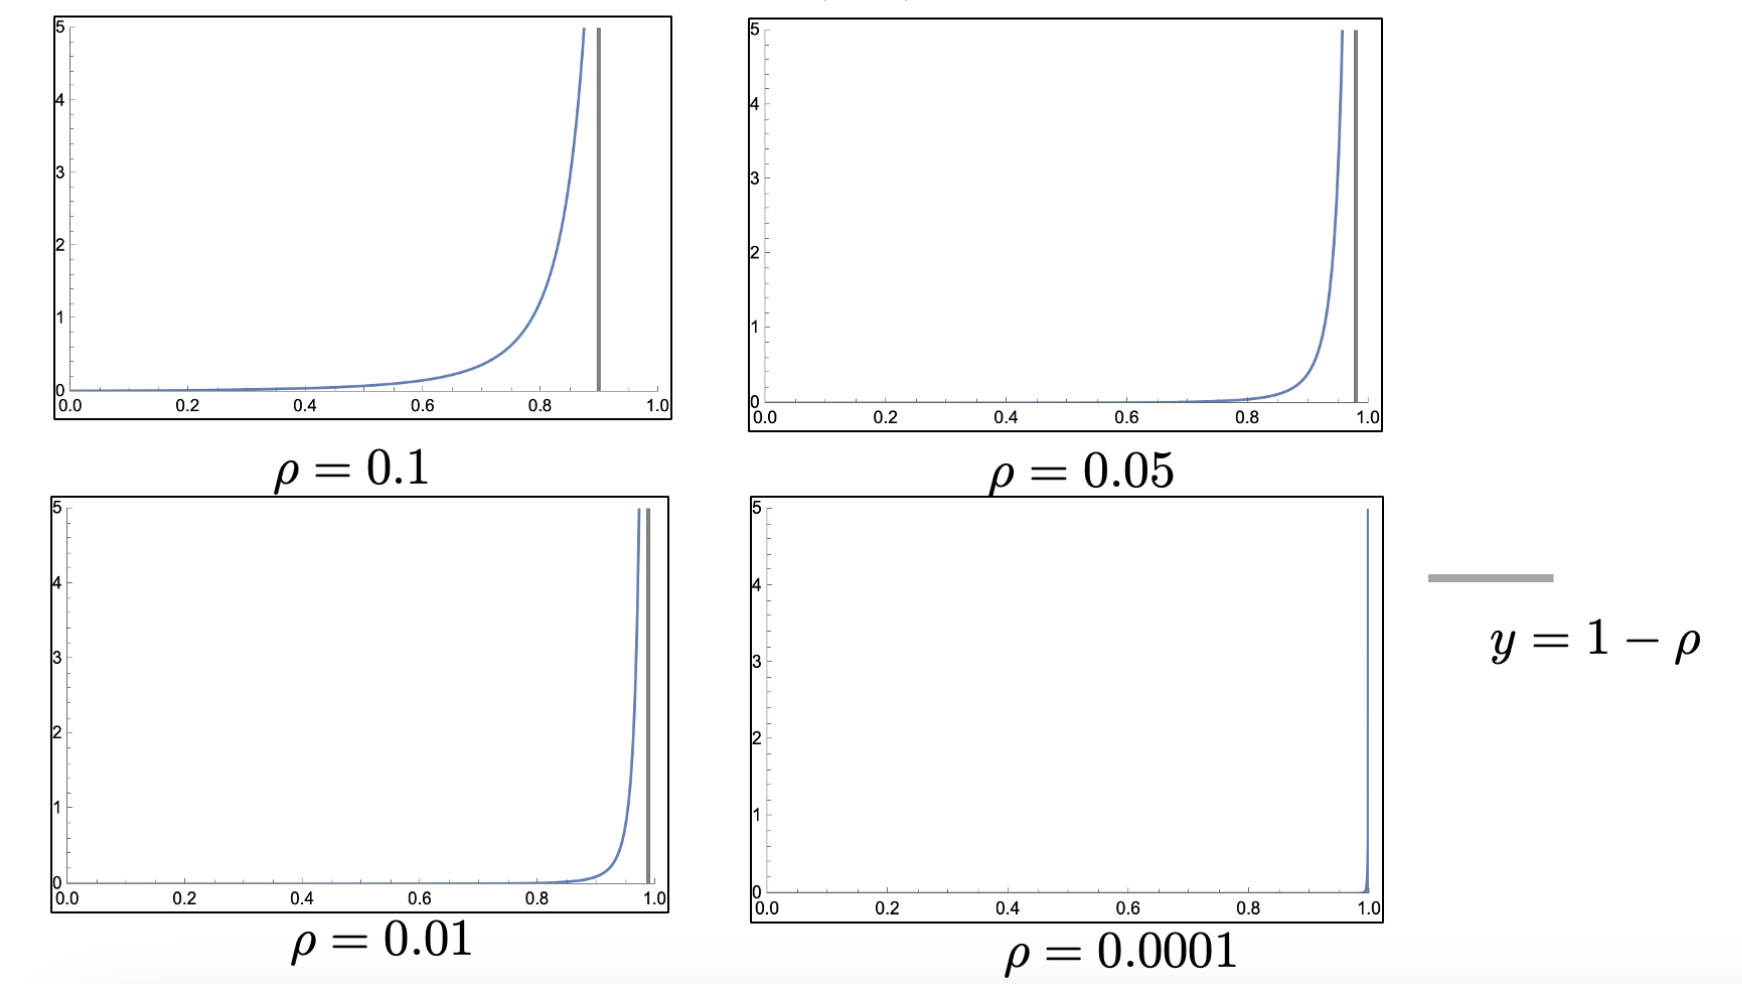
\includegraphics[width=0.8\textwidth]{figures/asymptotes.png}
    \caption{$\mrm{b\to u}$过程中电子能谱发散项的渐近行为}
    \label{fig:asp}
    \end{figure}
    本文用$\rho=0.1, 0.05, 0.01, 0.0001$为例，分析$g_\rho(y)(n=3)$的渐近行为。从图\ref{fig:asp}可知，$g_\rho(y)(n=3)$在$y=1-\rho$处发散，且发散行为处于渐近线的左侧。
    此外本文用光滑函数$t(y)$测试$g_\rho(y)$的积分行为，
    \begin{equation}
        \begin{aligned}
        \lim _{\rho \rightarrow 0} \int_0^{1-\rho} \mrm{d} y t(y) g_\rho(y) & =\frac{1}{(n-1)}\left[t(1)-\lim _{\rho \rightarrow 0} \int_0^{1-\rho} \mrm{d} y \frac{\mathrm{~d} t}{\mathrm{~d} y}(y) \frac{\rho^{n-1}}{(1-y)^{n-1}}\right] \\
        & =\frac{1}{(n-1)} t(1) .
        \end{aligned}
        \label{eq:asp_int}
        \end{equation}
    式\eqref{eq:asp_int}等号右边侧的第二项交换极限取积分次序，则被积函数等于零。最终$g_{\rho}(y)$可被等效为：
    \begin{equation}
        \begin{aligned}
        & \lim _{\rho \rightarrow 0} \frac{\rho^{n-1}}{(1-y)^n} \theta(1-\rho-y)=\frac{1}{(n-1)} \delta\left(1^{-}-y\right) \theta(1-y)=\frac{1}{(n-1)} \delta(1-y) \theta\left(1^{+}-y\right), \\
        & \lim _{\rho \rightarrow 0} \frac{\rho^{n-1}}{(1-y)^{n+1}} \theta(1-\rho-y)=-\frac{1}{(n-1)} \delta^{\prime}(1-y) \theta\left(1^{+}-y\right).
        \end{aligned}
        \label{eq:asp_replace}
        \end{equation}
    式\eqref{eq:asp_replace}中，$1^{+}$表示该值位于1的右侧领域，$1^{-}$表示该值位于1的左侧领域，结果表明$\delta$函数位于电子能量的积分区域。$\mrm{b}\to\mrm{u}$过程电子能谱为：
    \begin{equation}
        \begin{aligned}
        \frac{1}{\Gamma_0} \frac{\mathrm{~d} \Gamma}{\mathrm{~d} y}= & \left\{2(3-2 y) y^2 \theta(1-y)\right. \\
        & -\frac{2 \lambda_1}{m_\mrm{b}^2}\left[-\frac{5}{3} y^3 \theta(1-y)+\frac{1}{6} \delta(1-y) \theta\left(1^{+}-y\right)+\frac{1}{6} \delta^{\prime}(1-y) \theta\left(1^{+}-y\right)\right] \\
        & \left.-\frac{2 \lambda_2}{m_\mrm{b}^2}\left[-y^2(6+5 y) \theta(1-y)+\frac{11}{2} \delta(1-y) \theta\left(1^{+}-y\right)\right]\right\}
        \end{aligned}
        \end{equation}
    其中，$\Gamma_{0}=\frac{\left|V_{ub}\right|^2 G_F^2m_{b}^5}{192 \pi^3}$。
\subsection{第二种参数化方案}
    Andrea Albertia, Thorsten Ewerthb,等人在单圈水平上讨论了量纲五算符非微扰矩阵元对结构函数的修正\ct{Alberti:2012dn}。他们采用了一组新的运动学变量对相空间进行参数化。定义如下，
    \begin{equation}
            \hat{u}=\frac{(p-q)^2-m_{\mrm{c}}^2}{m_{\mrm{b}}^2},\quad
            \hat{q^2}=\frac{q^2}{m_{\mrm{b}}^2},\quad
            \hat{E}_{\mrm{e}}=\frac{E_{\mrm{e}}}{m_{\mrm{b}}}.\quad
        \label{eq:parameters_2}
    \end{equation}
    式\eqref{eq:parameters_2}中，$\hat{u}$是中间传播子的离壳度，在树图水平上$\hat{u}=0$.
    
    作为过渡，本节在树图水平上讨论包含量纲三算符和量纲五算符修正的电子能谱。一方面与上节结果进行交叉检验; 另一方面,本文在单圈水平上讨论量纲三算符对$\mrm{D\to X e^{+}\nu_e}$过程电子能谱的修正奠定必要的基础。

    衰变宽度关于无量纲化电子能量、轻子对转移动量平方和传播子离壳度的微分衰变宽度为：
    \begin{equation}
        \begin{aligned}
        \frac{\mathrm{d} \Gamma}{\mathrm{d} \hat{E}_{\mrm{\ell}} \, \mathrm{d} \hat{q}^2 \, \mathrm{d} \hat{u}} = & \frac{\mrm{G_F^2} m_{\mathrm{b}}^5 \left| \mrm{V_{\mathrm{cb}}} \right|^2}{16 \pi^3} \theta \left[ \frac{1}{2} \left( 1 - \rho + \hat{q}^2 - \hat{u} \right) - E_{\mathrm{e}} - \frac{\hat{q}^2}{4 E_{\mathrm{e}}} \right] \\
        & \times \left\{ \hat{q}^2 W_1 - \left[ 2 \hat{E}_{\mrm{\ell}}^2 - 2 \hat{E}_{\mrm{\ell}} \hat{q}_0 + \frac{\hat{q}^2}{2} \right] W_2 + \hat{q}^2 \left( 2 \hat{E}_{\mrm{\ell}} - \hat{q}_0 \right) W_3 \right\},
        \end{aligned}
        \label{eq:diffwidth_2}
        \end{equation}   
        其中的标量结构函数可以进行强相互作用耦合常数的微扰展开和底夸克质量负幂次的幂次展开：     
$$
W_i = W_i^{(0)} + \frac{\mu_{\mathrm{\pi}}^2}{2 m_{\mathrm{b}}^2} W_i^{(\mathrm{\pi}, 0)} + \frac{\mu_{\mathrm{G}}^2}{2 m_{\mathrm{b}}^2} W_i^{(\mathrm{G}, 0)} + \frac{C_F \alpha_s}{\pi} \left[ W_i^{(1)} + \frac{\mu_{\mathrm{\pi}}^2}{2 m_{\mathrm{b}}^2} W_i^{(\mathrm{\pi}, 1)} + \frac{\mu_{\mathrm{G}}^2}{2 m_{\mathrm{b}}^2} W_i^{(\mathrm{G}, 1)} \right]+\cdots.
$$
本节忽略高阶修正仅考虑树图水平贡献。其中树图水平上的结构函数 $W_{i}, i=1,2,3$ 为：
$$
W_i^{(0)}=w_i^{(0)} \delta(\hat{u}) ; \quad w_1^{(0)}=2 E_0, \quad w_2^{(0)}=4, \quad w_3^{(0)}=2.
$$
树图水平上量纲五算符(动力学算符)对应的的结构函数 $W_{i}^{(\pi,0)}, i=1,2,3$ 如下所示：
\begin{equation}
W_i^{(\pi, 0)}=w_i^{(\pi, 0)} \delta(\hat{u})+w_i^{(\pi, 1)} \delta^{\prime}(\hat{u})+w_i^{(\pi, 2)} \delta^{\prime \prime}(\hat{u}),
\end{equation}
$$
\begin{array}{lll}
w_1^{(\pi, 0)}=\frac{8}{3}\left(1-E_0\right), & w_1^{(\pi, 1)}=\frac{4}{3} E_0\left(1-E_0\right), & w_1^{(\pi, 2)}=\frac{2}{3} E_0 \lambda_0 ,\\
w_2^{(\pi, 0)}=0, & w_2^{(\pi, 1)}=-8\left(1-E_0\right), & w_2^{(\pi, 2)}=\frac{4}{3} \lambda_0 , \\
w_3^{(\pi, 0)}=-2, & w_3^{(\pi, 1)}=-\frac{4}{3}\left(1-E_0\right), & w_3^{(\pi, 2)}=\frac{2}{3} \lambda_0,
\end{array}
$$
树图水平上量纲五算符(色磁算符)对应的结构函数 $W_{i}^{(G,0)}, i=1,2,3$ 如下所示：
\begin{equation}
    W_i^{(\mathrm{G}, 0)} = w_i^{(\mathrm{G}, 0)} \delta(\hat{u}) + w_i^{(\mathrm{G}, 1)} \delta^{\prime}(\hat{u});
    \end{equation}
$$
\begin{array}{ll}
w_1^{(\mathrm{G}, 0)} = -\frac{4}{3} \left( 2 - 5 E_0 \right), & w_1^{(\mathrm{G}, 1)} = -\frac{4}{3} \left( E_0 + 3 E_0^2 + \frac{1}{2} \lambda_0 \right) ; \\
w_2^{(\mathrm{G}, 0)} = 0, & w_2^{(\mathrm{G}, 1)} = \frac{8}{3} \left( 3 - 5 E_0 \right) ; \\
w_3^{(\mathrm{G}, 0)} = \frac{10}{3}, & w_3^{(\mathrm{G}, 1)} = -\frac{4}{3} \left( 1 + 5 E_0 \right) .
\end{array}
$$

其中，$E_0=\frac{1}{2}\left(1+\rho-\hat{q}^2\right)$, $\lambda_0=4\left(E_0^2-\rho\right)$.

对于$(E_{\mathrm{e}}, E_{\mathrm{\nu_e}}, q^2)$这组运动学变量，$E_{\mathrm{\nu_e}}$的下限是$\frac{\hat{q^{2}}}{4 E_{\mrm{e}}}$.  当固定$E_{\mrm{e}}, q^2$, 中间传播子离壳度$\hat{u}$与中微子能量$E_{\mrm{\nu_{e}}}$存在一一对应的关系。即$$\hat{u} = 1 + \hat{q^2} - \rho - 2 \left( \hat{E_{\mathrm{e}}} + \hat{E}_{\mathrm{\nu_e}} \right).$$ $\hat{u}$的运动学区域的上限是$(1 - \rho + \hat{q^2}) - 2 \hat{E_{\mathrm{e}}} - \frac{\hat{q^2}}{2 E_{\mathrm{e}}}$，类似地,引入$$\theta\left[\frac{1}{2}(1-\rho+\hat{q^2}-\hat{u})-E_{\mrm{e}}-\frac{\hat{q^{2}}}{4 E_{\mrm{e}}}\right],$$将对积分区域解析延拓到正无穷,这是式\eqref{eq:diffwidth_2}中Heavside-theta项。
\begin{figure}[h!]
    \centering
    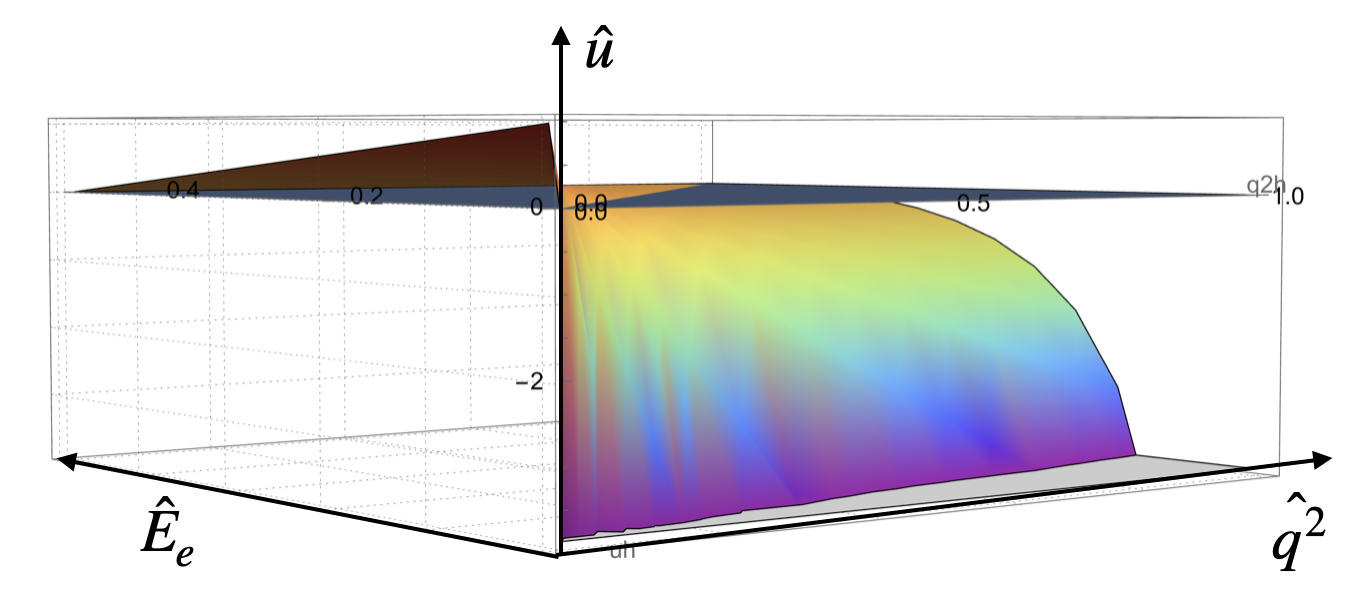
\includegraphics[width=0.8\textwidth]{figures/phase2.png}
    \caption{中间传播子离壳度的积分区域}
\end{figure}

完成对$\hat{u}$的积分\footnote{$\hat{q^{0}}$表示无量纲化的中微子能量和电子能量之和， 这时$\hat{u}=1+\hat{q^{2}}-\rho-2\hat{q^{0}}$.具体地， 树图水平对应于$\hat{u}=0$，$\hat{q^{0}}$是关于$\hat{u}$的函数，在分部积分的过程中，$\hat{q^{0}}(\hat{u})$在零点关于$\hat{u}$的导数必须在先对$\hat{q^{0}}(\hat{u})$求导，然后再取导函数在零点处的值。}, Heavside-Theta函数变成$\theta\left(\frac{(4 \hat{E}_\mrm{e} - 2 (1 - \rho)) \hat{E}_\mrm{e}}{2 \hat{E}_\mrm{e} - 1}\right)$, 这将给出关于$\hat{q^{2}}$的积分区域，完成对$\hat{q^{2}}$的积分之后，可得了$\mrm{\bar{B}}\to \mrm{X_{c}}e\nu$过程的电子能谱为：
\begin{equation}
    \begin{aligned}
        \frac{1}{\Gamma_{0}} \frac{d \Gamma}{d \hat{E}_{\mathrm{e}}} = \{ & 16 \hat{E}_{\mathrm{e}}^2 (3 - 4 \hat{E}_{\mathrm{e}}) - 48 \hat{E}_{\mathrm{e}}^2 \rho - \frac{48 \hat{E}_{\mathrm{e}}^2 \rho^2}{(1 - 2 \hat{E}_{\mathrm{e}})^2} + \frac{16 \hat{E}_{\mathrm{e}}^2 (3 - 2 \hat{E}_{\mathrm{e}}) \rho^3}{(1 - 2 \hat{E}_{\mathrm{e}})^3} \\
        & - \frac{32 \mu_{\pi}^2}{3 m_{\mathrm{b}}^2} \hat{E}_{\mathrm{e}}^3 \left[ 5 + \frac{3 (5 - 4 \hat{E}_{\mathrm{e}})}{(1 - 2 \hat{E}_{\mathrm{e}})^4} \rho^2 - \frac{4 (2 \hat{E}_{\mathrm{e}}^2 - 5 \hat{E}_{\mathrm{e}} + 5)}{(1 - 2 \hat{E}_{\mathrm{e}})^5} \rho^3 \right] \\
        & + \frac{32 \mu_{\mathrm{G}}^2}{3 m_{\mathrm{b}}^2} \hat{E}_{\mathrm{e}}^2 \left[ 3 + 5 \hat{E}_{\mathrm{e}} + \frac{3 (4 \hat{E}_{\mathrm{e}} - 3)}{(1 - 2 \hat{E}_{\mathrm{e}})^2} \rho - \frac{9 (1 - \hat{E}_{\mathrm{e}})}{(1 - 2 \hat{E}_{\mathrm{e}})^3} \rho^2 + \frac{5 (2 \hat{E}_{\mathrm{e}}^2 - 4 \hat{E}_{\mathrm{e}} + 3)}{(1 - 2 \hat{E}_{\mathrm{e}})^4} \rho^3 \right] \\
        & \} \theta \left( \frac{1 - \rho}{2} - \hat{E}_{\mathrm{e}} \right).
    \end{aligned}
\end{equation}

整体会留下另一个 Heavside-Theta函数$\theta(\frac{1-\rho}{2}-\hat{E}_{e})$对$\hat{E}_{e}$积分区域进行限制。关于无量纲化电子能量的积分，Heavside-Theta函数给出的约束是$\left[0,\frac{1-\rho}{2}\right]$,最终可得$\mrm{B\to X_{c} e\nu}$过程的衰变宽度为：
\begin{equation}
    \begin{aligned}
    \frac{\Gamma}{\Gamma_{0}}=&1 - 8 \rho + 8 \rho^3 - \rho^4 - 12 \rho^2 \ln\rho\\
    &-\mu_{\pi}^2\left[1 - 8 \rho + 8 \rho^3 - \rho^4 - 12 \rho^2 \ln\rho\right]\\
    &+\mu_{G}^2\left[3 - 8 \rho + 24 \rho^2 - 24 \rho^3 + 5 \rho^4 + 12 \rho^2 \ln\rho\right],\\
\end{aligned}
\end{equation}
该结果与式\eqref{eq:decaywidth_B_1}保持一致。
\subsection{两种参数化方案之间的转换}
为了方便两种参数化方案之间进行交叉检验，本节讨论两种参数化方案下的结构函数、微分衰变宽度和衰变宽度之间的转换关系。

\subsubsection{第一种参数化方案}
$\mrm{\bar{B}}$介子半轻单举衰变宽度为：
\begin{equation}
    \begin{aligned}
        \Gamma =  \int \frac{\mrm{d}^{3} \vec{p_{\mathrm{e}}}}{(2 \pi)^{3} 2 E_{\mathrm{e}}} &\frac{\mrm{d}^{3} \vec{p_{\mathrm{X_{c}}}}}{(2 \pi)^{3} 2 E_{\mathrm{X_{c}}}} \frac{\mrm{d}^{3} \vec{p_{\nu_{e}}}}{(2 \pi)^{3} 2 E_{\mathrm{\nu_e}}}\times\\
         &\sum_{X_{\mathrm{c}}} \sum_{\substack{\text{lepton} \\ \text{spins}}} \frac{\left|\left\langle \mrm{X_{\mathrm{c}} \mrm{e} \mrm{\bar{\nu}}_{\mathrm{e}} }\left| H_W \right| \mrm{\bar{B}} \right\rangle \right|^2}{2 m_{\mathrm{B}}} (2 \pi)^4 \delta^4\left[p_{\mathrm{B}} - \left(p_{\mathrm{e}} + p_{\mathrm{\nu_e}}\right) - p_{X_{\mathrm{c}}}\right],
    \end{aligned}
\end{equation}
经过适当的相空间积分后，可得三微分衰变宽度为：
\begin{equation}
    \frac{\mathrm{d} \Gamma}{\mathrm{d} q^2 \, \mathrm{d} E_{\mathrm{e}} \, \mathrm{d} E_{\mathrm{\nu_e}}} = \frac{1}{4} \sum_{\mrm{X}_{\mathrm{c}}} \sum_{\substack{\text{lepton} \\ \text{spins}}} \frac{\left|\left\langle\mrm{ X e \bar{v}_{\mathrm{e}} }\left| H_W \right| \mrm{\bar{B} }\right\rangle \right|^2}{2 m_{\mathrm{B}}} \delta^4 \left[ p_{\mathrm{B}} - \left( p_{\mathrm{e}} + p_{\mathrm{\nu_e}} \right) - p_{X_{\mathrm{c}}} \right] .
    \end{equation}    
其中，
\begin{equation}
    \begin{aligned}
    & \frac{1}{4} \sum_{{X_\mathrm{c}}} \sum_{\substack{\text{lepton} \\ \text{spins}}} \frac{\left|\left\langle \mrm{X_{\mathrm{c}} e \bar{\nu}_{\mathrm{e}} }\left| H_W \right| \mrm{\bar{B}} \right\rangle \right|^2}{2 m_{\mathrm{B}}} (2 \pi)^3 \delta^4 \left[ p_{\mathrm{B}} - \left( p_{\mathrm{e}} + p_{\mathrm{\nu_e}} \right) - p_{X_{\mathrm{c}}} \right] \\
    & \quad = 2 \mrm{G_F^2} \left| V_{\mathrm{c b}} \right|^2 W_{\alpha \beta} L^{\alpha \beta},
    \end{aligned}
    \end{equation}
    
其中有关强子张量$W^{\prime}$的定义如下：
\begin{equation}
W_{\alpha \beta}^{\prime}=\operatorname{Im}(\frac{\mrm{i}}{2m_{\mrm{B}}\pi} \int \mrm{d}^4 x e^{-i q \cdot x} \left\langle\mrm{\bar{B}}\left|\operatorname{T}\left[J_{\mrm{L} \alpha}^{\dagger}(x) J_{\mrm{L} \beta}(0)\right]\right|\mrm{ \bar{B}}\right\rangle)
\end{equation}
在微扰论领头阶，
\begin{equation}
    \begin{aligned}
    W_{\alpha \beta}^{\prime} = & \sum_{\mrm{X}_{\mathrm{c}}} (2 \pi)^3 \delta^4 \left( p_{\mathrm{B}} - q - p_{X_{\mathrm{c}}} \right) \frac{1}{2 m_{\mathrm{B}}} \\
    & \times \left\langle \mrm{\bar{B} }\left( p_{\mathrm{B}} \right) \left| J_\mrm{L}^{\dagger \alpha} \right| \mrm{X_{\mathrm{c}} }\left( p_{X_{\mathrm{c}}} \right) \right\rangle \left\langle X_{\mathrm{c}} \left( p_{\mrm{X_{\mathrm{c}}}} \right) \left| J_\mrm{L}^\beta \right| \mrm{\bar{B}} \left( p_{\mathrm{B}} \right) \right\rangle,
    \end{aligned}
    \end{equation}    
基于洛伦兹对称性和电荷共轭对称性，可将$W_{\alpha \beta}^{\prime}$分解为
\begin{equation}
    m_{b}W^{\prime}_{\alpha \beta}=-g_{\alpha \beta} m_{b}W^{\prime}_1+v_\alpha v_\beta m_{b}W_2^{\prime}-i \epsilon_{\alpha \beta \mu \nu} v^\mu q^\nu m_{b} W_3^{\prime}+q_\alpha q_\beta m_{b} W_4^{\prime}+\left(v_\alpha q_\beta+v_\beta q_\alpha\right)m_{b} W_5^{\prime}
\end{equation}
轻子张量约定为：
\begin{equation}
L^{\alpha \beta}=2\left(p_e^\alpha p_{v_e}^\beta+p_e^\beta p_{v_e}^\alpha-g^{\alpha \beta} p_e \cdot p_{v_e}-i \epsilon^{\eta \beta \lambda \alpha} p_{e \eta} p_{v_e \lambda}\right)
\end{equation}
强子张量和轻子张量进行洛伦兹指标缩并之后，W4和W5消失并可得三微分衰变宽度的表达式为：
\begin{equation}
    \begin{aligned}
    \frac{\mathrm{d} \Gamma}{\mathrm{d} q^2 \, \mathrm{d} E_{\mathrm{e}} \, \mathrm{d} E_{\mathrm{\nu_e}}} = & \frac{G_F^2 \left| \mrm{V}_{\mathrm{cb}} \right|^2}{2 \pi^3} \left[ W_1^{\prime} q^2 + W_2^{\prime} \left( 2 E_{\mathrm{e}} E_{\mathrm{\nu_e}} - \frac{q^2}{2} \right) \right. \\
    & \left. + W_3^{\prime} q^2 \left( E_{\mathrm{e}} - E_{\mathrm{\nu_e}} \right) \right] \theta \left( 4 E_{\mathrm{e}} E_{\mathrm{\nu_e}} - q^2 \right)
    \end{aligned}
    \end{equation}    
对上式做无量纲化处理\footnote{$m_{b}^{5}=m_{b}^{4}\cdot m_{b}$,乘积第一项来自于微分衰变宽度表达式的左边无量纲化，第二项来自于结构函数的无量纲化。注意，$4\tilde{W_{i}}^{\prime}=W_{i}$}，
\begin{equation}
    \begin{aligned}
    \frac{\mathrm{d} \Gamma}{\mathrm{d} \hat{q}^2 \, \mathrm{d} \hat{E}_{\mathrm{e}} \, \mathrm{d} \hat{E}_{\mathrm{\nu_e}}} = & \frac{G_F^2 \left| V_{\mathrm{c b}} \right|^2 m_{\mathrm{b}}^5}{2 \pi^3} \left[ \tilde{W_1}^{\prime} \hat{q}^2 + \tilde{W_2}^{\prime} \left( 2 \hat{E}_{\mathrm{e}} \hat{E}_{\mathrm{\nu_e}} - \frac{\hat{q}^2}{2} \right) \right. \\
    & \left. + \tilde{W_3}^{\prime} \hat{q}^2 \left( \hat{E}_{\mathrm{e}} - \hat{E}_{\mathrm{\nu_e}} \right) \right] \theta \left( 4 \hat{E}_{\mathrm{e}} \hat{E}_{\mathrm{\nu_e}} - \hat{q}^2 \right)
    \end{aligned}
    \label{eq2:12}
    \end{equation}    
\subsubsection{第二种参数化方案}
$\mrm{\bar{B}}\to\mrm{X_c e\nu}$过程的强子张量约定如下
\begin{equation}
    W_{\alpha \beta}=\frac{2}{\pi}\text{Im}\{\frac{i}{m_{B}} \int d^4 x e^{-i q \cdot x} \bra{\bar{B}}T\left[J_{L \alpha}^{\dagger}(x) J_{L \beta}(0)\right] \ket{\bar{B}}\}
    \end{equation}
基于洛伦兹对称性和电荷共轭对称性，$W_{\alpha\beta}$可进行如下的张量分解：
    \begin{equation}
         m_{\mrm{b}}W_{\alpha \beta}=-g_{\alpha \beta}W_1+v_\alpha v_\beta W_2-i \epsilon_{\alpha \beta \mu \nu} v^\mu q^\nu  W_3+q_\alpha q_\beta W_4+\left(v_\alpha q_\beta+v_\beta q_\alpha\right) W_5
    \end{equation}
    此外，标量结构函数关于强相互作用耦合常数的微扰展开和关于底夸克质量负幂次的幂次展开为：
    \begin{equation}
        W_i = W_i^{(0)} + \frac{\mrm{\mu_{\pi}^2}}{2 m_{\mathrm{b}}^2} W_i^{(\pi, 0)} + \frac{\mrm{\mu_{\mathrm{G}}^2}}{2 m_{\mathrm{b}}^2} W_i^{(\mathrm{G}, 0)} + \frac{C_F \alpha_s}{\pi} \left[ W_i^{(1)} + \frac{\mrm{\mu_{\pi}^2}}{2 m_{\mathrm{b}}^2} W_i^{(\pi, 1)} + \frac{\mrm{\mu_{\mathrm{G}}^2}}{2 m_{\mathrm{b}}^2} W_i^{(\mathrm{G}, 1)} \right]
        \end{equation}        
    其中的非微扰矩阵元可进行如下参数化：
    \begin{equation}
        \begin{aligned}
            \mrm{\mu_\pi^2}&=\frac{-1}{2 m_B}\left\langle\bar{B}(v)\left|\bar{b}_v(i D)^2 b_v\right| \bar{B}(v)\right\rangle,\\
            \mrm{\mu_G^2}&=-\frac{1}{6 m_B}\left\langle\bar{B}(v)\left|\bar{b}_v \frac{g_s}{2} G_{\mu \nu} \sigma^{\mu \nu} b_v\right| \bar{B}(v)\right\rangle,
        \end{aligned}
    \end{equation}
    其中，$D_\mu=\partial_\mu+i g_s G_\mu^a T^a$是协变微分算子，$\mrm{G_{\mu\nu}}$是规范场强张量，$\mrm{b_{v}}$是静止底夸克场。$\lambda_1, \lambda_2$定义于渐进HQET区域，但实际计算过程往往位于有限夸克质量态，两者的差异如下：
    $$\mrm{\mu_\pi^2=-\lambda_1}+\mathcal{O} \left(1 / m_\mrm{b}\right)\quad \mrm{\mu_G^2=3 \lambda_2}+\mathcal{O}\left(1 / m_\mrm{b}\right)$$
   
    两种参数化方案之间关于结构函数约定的全局差异如下\footnote{这里的变量替换涉及到Dirac-delta函数及其高阶导函数，需要考虑正确地处理 Delta 函数导数的所有零点并考虑额外的雅可比行列式。$n= 0，1，2$分指别至Dirac delta函数，一阶导函数，二阶导函数}：
    \begin{equation}
        \begin{aligned}
                W_{\alpha \beta}(q^{2}, \hat{u}) &= 4 \cdot 2^{n+1} (-1)^{n} W^{\prime}_{\alpha \beta}(q^{2}, q^{0}) \\
                W_{i} &= 4 m_{\mathrm{b}} \cdot 2^{n+1} (-1)^{n} W_{i}^{\prime}(q^{2}, q^{0}), \, i = 1, 2 \\
                W_{3} &= 4 m_{\mathrm{b}}^{2} \cdot 2^{n+1} (-1)^{n} W_{3}^{\prime}(q^{2}, q^{0}) \\
                W_{4} &= 4 m_{\mathrm{b}}^{3} \cdot 2^{n+1} (-1)^{n} W_{4}^{\prime}(q^{2}, q^{0}) \\
                W_{5} &= 4 m_{\mathrm{b}}^{2} \cdot 2^{n+1} (-1)^{n} W_{5}^{\prime}(q^{2}, q^{0}) \\
        \end{aligned}
    \end{equation}    
    
    $\mrm{\bar{B}\to X_{c}e\nu}$过程在新的参数化方案下的三微分衰变宽度为： 
    \begin{equation}
    \begin{aligned}
    \frac{\mrm{d} \Gamma}{\mrm{d} \hat{E}_{\mrm{\ell}} \mrm{d} \hat{q}^2 \mrm{d} \hat{u}}= & \frac{\mrm{G_F^2} m_\mrm{b}^5\mrm{\left|V_{c b}\right|^2}}{16 \pi^3} \theta\left(\hat{u}_{+}-\hat{u}\right) \times \\
    & \times\left\{\hat{q}^2 W_1-\left[2 \hat{E}_{\mrm{\ell}}^2-2 \hat{E}_{\mrm{\ell}} \hat{q}_0+\frac{\hat{q}^2}{2}\right] W_2+\hat{q}^2\left(2 \hat{E}_{\mrm{\ell}}-\hat{q}_0\right) W_3\right\},
    \end{aligned}
    \label{eq:2:23}
    \end{equation}
    从\ref{eq2:12}出发，简单讨论\ref{eq:2:23}与\ref{eq2:12}之间的一致性\footnote{不能简单地认为\ref{eq:2:24}和\ref{eq:2:25}在三微分衰变宽度上成立（尽管在树图阶的领先幂次看起来是这样）。一般地, 将三微分衰变宽度的表达式分为$\delta$项、$\delta^{\prime}$项、$\delta^{\prime\prime}$项，则\ref{eq:2:24}分别取n=0，1，2时，等号对应成立。}
    \begin{equation}
        \begin{aligned}
    \frac{\mathrm{d} \Gamma}{\mathrm{d} \hat{q}^2 \, \mathrm{d} \hat{E}_{\mathrm{e}} \, \mathrm{d} \hat{E}_{\mathrm{\nu_e}}} = & \frac{G_F^2 \left| V_{\mathrm{c b}} \right|^2 m_{\mathrm{b}}^5}{4 \cdot 2 \pi^3 \cdot 2^{n+1} (-1)^n} \left[ W_1 \hat{q}^2 + W_2 \left( 2 \hat{E}_{\mathrm{e}} \hat{E}_{\mathrm{\nu_e}} - \frac{\hat{q}^2}{2} \right) \right. \\
    & \left. + W_3 \hat{q}^2 \left( \hat{E}_{\mathrm{e}} - \hat{E}_{\mathrm{\nu_e}} \right) \right] \theta \left( 4 \hat{E}_{\mathrm{e}} \hat{E}_{\mathrm{\nu_e}} - \hat{q}^2 \right) \\
    = & \frac{G_F^2 \left| \mrm{V_{\mathrm{c b}}} \right|^2 m_{\mathrm{b}}^5}{16 \pi^3 (-2)^n} \left\{ \hat{q}^2 W_1 - \left[ 2 \hat{E}_{\ell}^2 - 2 \hat{E}_{\ell} \hat{q}_0 + \frac{\hat{q}^2}{2} \right] W_2 + \hat{q}^2 \left( 2 \hat{E}_{\ell} - \hat{q}_0 \right) W_3 \right\}
    \end{aligned}
    \label{eq:2:24}
\end{equation}
    n取0，对应结构函数里只含有Dirac delta函数（树图阶的领先幂次），这时式\eqref{eq:2:24}与式\eqref{eq:2:23}形式上保持一致。若结构函数中存在Dirac Delta函数的高阶导函数项，则做变量替换需要谨慎考虑Dirac Delta函数的零点和额外的雅各比行列式贡献。其主要思路是：从微分衰变宽度出发，用两个准两体末态相空间积分来处理三体衰变末态，积分掉多余的运动学变量，保留$\hat{E}_{\mrm{l}}$, $\hat{u}$, $q^{2}$，可得式\eqref{eq:2:23}。而式\eqref{eq2:12}的基本思路是：从衰变宽度出发，插入$E_{l}$, $E_{\nu}$, $q^{2}$的Dirac $\delta$函数，抽取出关于$E_{\mrm{l}}$,  $E_{\mrm{\nu_e}}$，$q^{2}$的微分衰变宽度。
    \begin{equation}
        \frac{\mathrm{d} \Gamma}{\mathrm{d} \hat{q}^2 \, \mathrm{d} \hat{E}_{\mathrm{e}} \, \mathrm{d} \hat{E}_{\mathrm{\nu_e}}} = \left( - \frac{1}{2} \right)^n \frac{\mrm{d} \Gamma}{d \hat{E}_{\mrm{\ell}} \, \mrm{d} \hat{q}^2 \, \mrm{d} \hat{u}}
        \label{eq:2:25}
    \end{equation}    
    \begin{equation}
        \frac{\mathrm{d} \Gamma}{\mathrm{d} \hat{q}^2 \, \mathrm{d} \hat{E}_{\mathrm{e}}} = \frac{\mrm{d} \Gamma}{ \mathrm{d} \hat{E}_{\mrm{\ell}} \,  \mathrm{d}  \hat{q}^2}
        \label{eq:2:25}
    \end{equation}    
    关于\ref{eq:2:25}\footnote{这里的$(-\frac{1}{2})^{n}$来自于Dirac delta函数中变量替换对雅各比行列式的贡献，即上Dirac delta函数的零点和额外的雅各比行列式），树图阶没有来自被积函数变量替换带来的雅各比行列式。}, 由于分部积分引入关于积分结果的冗余自由度，即存在多种等价形式的积分结果，即\footnote{\ref{eq:2:27}第二行的公式是的$f^{\prime}(y)$的意思是先做x到y的替换，再对y整体求导。另一个公式则不用考虑这个次序：$$f(x)\delta^{\prime\prime}(x-y)=f(y)\delta^{\prime\prime}(x-y)-2f^{\prime}(x)\delta^{\prime}(x-y)-f^{\prime}(x)\delta(x-y)$$这个公式是对$f(x) \delta(x-y)=f(y) * \delta(x-y)$求两次关于x的导数整理而来。}:
    \begin{equation}
    \begin{aligned}
    & f(x) \delta^{\prime}(x-y)=f(y) * \delta^{\prime}(x-y)-f^{\prime}(y) \delta(x-y) \\
    & f(x) \delta^{\prime \prime}(x-y)=f(y) * \delta^{\prime \prime}(x-y)-2 f^{\prime}(y) \delta^{\prime}(x-y)+f^{\prime \prime}(y) \delta(x-y)
    \end{aligned}
    \label{eq:2:27}
    \end{equation} 
    基于以上讨论，可实现两组参数化方案之间的检验。
\subsection{粲强子单举衰变过程的电子能谱及衰变宽度}
粲强子半轻单举衰变相比于底强子半轻单举衰变的区别在于轻子部分，前者轻子末态是正电子和电子中微子，而后者轻子末态是电子和反电子中微子。这一区别反映在轻子张量上Levi-theta项上，最终表现为微分衰变宽度中$W_{3}$项。因此本节直接给出树图水平上精确至量纲五算符非微扰矩阵元水平的$\mrm{D\to X e^{+}\nu_{e}}$过程电子能谱，
\begin{equation}
    \begin{aligned}
        \frac{1}{\Gamma_{0}} \frac{\mathrm{d} \Gamma}{\mathrm{d} \hat{E}_{\mathrm{e}}} = & 96 \hat{E}_{\mathrm{e}}^2 (1 - 2 \hat{E}_{\mathrm{e}}) \theta\left( \frac{1}{2} - \hat{E}_{\mathrm{e}} \right) \\
        & + \frac{8 \mu_{\pi}^2}{m_{\mathrm{c}}^2} \hat{E}_{\mathrm{e}}^3 \left[ 20 \hat{E}_{\mathrm{e}} + (5 - 6 \hat{E}_{\mathrm{e}}) \delta \left( \frac{1}{2}^{-} - \hat{E}_{\mathrm{e}} \right) \right] \theta\left( \frac{1}{2} - \hat{E}_{\mathrm{e}} \right) \\
        & - \frac{32 \mu_{\mathrm{G}}^2}{m_{\mathrm{c}}^2} \hat{E}_{\mathrm{e}}^2 (3 - 5 \hat{E}_{\mathrm{e}}) \theta\left( \frac{1}{2} - \hat{E}_{\mathrm{e}} \right) \\
        & + \cdots,
    \end{aligned}
    \label{eq:c_electron_sp}
\end{equation}
式\eqref{eq:c_electron_sp}中，$\hat{E}_{e}=\frac{E_{\mrm{e}}}{m_{\mrm{c}}}$, $\Gamma_{0}=\frac{\mrm{G_F^2} m_\mrm{c}^5 \mrm{V}_{\text{CKM}}}{192\pi^3}$, $\frac{1}{2}^{-}$表示该值位于1/2的左侧邻域，第一行是量纲三算符对电子能谱的贡献，第二行和第三行分别是量纲五算符$\mu_{\pi}^{2}$和$\mu_{\mrm{G}}^{2}$对电子能谱的贡献。基于该电子能谱进行加权积分，可得衰变宽度、电子能量矩等多种物理可观测量。例如衰变宽度,
\begin{equation}
    \frac{1}{\Gamma_{0}}\Gamma=1-\frac{1}{2 m_{c}^2}\mu_{\pi}^{2}-\frac{3}{2 m_{c}^2}\mu_{G}^{2}
    \label{eq:decaywidth_C_tree}
\end{equation}
式\eqref{eq:decaywidth_C_tree}中, $\mrm{V_{\text{CKM}}}$主要包含两部分，即$\mrm{V_{\text{cs}}}$和$\mrm{V_{\text{cd}}}$,末态夸克质量取零极限对应于$\mrm{c\to d}$跃迁；对于$\mrm{c\to s}$跃迁，由于奇异夸克质量并非特别小，需要作为软自由度进行保留。本文采用Mannel等人的结果\ct{Fael:2019umf}来考虑末态有限夸克质量效应对粲强子半轻单举衰变的修正。
\section{微扰修正}
本节讨论$\mrm{D\to X e^{+}\nu_{e}}$过程单圈水平上领先幂次的修正：从$\mrm{B\to X_{\text{c}}e\nu}$过程的领先幂次出发，取末态夸克零质量极限可得$\mrm{B\to X_{\text{u}}e\nu}$过程的结构函数。此外讨论$\mrm{B\to X_{\text{u}}e\nu}$的相空间解析积分，得到$\mrm{B\to X_{\text{u}}e\nu}$过程的电子能谱。基于粲强子与底强子单举衰变的区别，可得粲强子单举衰变的电子能谱。由于重夸克展开在电子能量末端失效，因此需要对电子能谱进行加权积分，得到衰变宽度、电子能量矩等各种具有非微扰参数依赖的物理量。

\subsection{单圈水平上$\mrm{B\to X_{\text{c}}e\nu}$过程的领先幂次修正}
$\mrm{B\to X_{\text{c}}e\nu}$过程的微分衰变宽度是
\begin{equation}
    \begin{aligned}
    \frac{\mathrm{d} \Gamma}{\mathrm{d} \hat{E}_{\ell} \, \mathrm{d} \hat{q}^2 \, \mathrm{d} \hat{u}} = & \frac{G_F^2 m_{\mathrm{b}}^5 \left| \mrm{V}_{\mathrm{c b}} \right|^2}{16 \pi^3} \\
    & \times \left\{ \hat{q}^2 W_1 - \left[ 2 \hat{E}_{\ell}^2 - 2 \hat{E}_{\ell} \hat{q}_0 + \frac{\hat{q}^2}{2} \right] W_2 + \hat{q}^2 \left( 2 \hat{E}_{\ell} - \hat{q}_0 \right) W_3 \right\} \\
    & \times \theta \left[ \frac{1}{2} \left( 1 - \rho + \hat{q}^2 - \hat{u} \right) - \hat{E}_{\mathrm{e}} - \frac{\hat{q}^2}{4 \hat{E}_{\mathrm{e}}} \right],
    \end{aligned}
\end{equation}
其中，$W_{i}, i=1, 2, 3$是该过程标量结构函数，它可以被强相互作用耦合常数与底夸克质量负幂次进行双重展开，
\begin{equation}
    W_i = W_i^{(0)} + \frac{\mu_{\pi}^2}{2 m_{\mathrm{b}}^2} W_i^{(\pi, 0)} + \frac{\mu_{\mathrm{G}}^2}{2 m_{\mathrm{b}}^2} W_i^{(\mathrm{G}, 0)} + \frac{\alpha_s}{\pi} \left[ \left[ C_F W_i^{(1)} \right] + C_F \frac{\mu_{\pi}^2}{2 m_{\mathrm{b}}^2} W_i^{(\pi, 1)} + \frac{\mu_{\mathrm{G}}^2}{2 m_{\mathrm{b}}^2} W_i^{(\mathrm{G}, 1)} \right]+\cdots,
\end{equation}
其中，$W_{i}^{(1)}$可由在单圈水平上完整理论和有效理论之间的算符匹配得到。该匹配过程基于图\ref{fig:Matching_NLO}完成，
\begin{figure}[h!]
    \centering
    
\includegraphics[width=0.7\textwidth]{MatchingNLO.png}
    \caption{两点关联函数的单圈修正\ct{Aquila:2005hq}}
    \label{fig:Matching_NLO}
\end{figure}

P. Gambino等人05年的工作中\ct{Aquila:2005hq}, 讨论了$\mrm{B\to X_{\text{c}}e\nu}$单圈水平上领先幂次对结构函数的修正:
\begin{equation}
    W_i^{(1)}=w_i^{(0)}\left\{S_i \delta(\hat{u})-2\left(1-E_0 I_1\right)\left[\frac{1}{\hat{u}}\right]_{+}+\frac{\theta(\hat{u})}{(\rho+\hat{u})}\right\}+R_i \theta(\hat{u}),
    \end{equation}
其中， $S_i=S+\Delta_i$，
$S=2 E_0\left(I_{2,0}-I_{4,0}\right)-1-\frac{1-\rho-6 \hat{q}^2}{4 \hat{q}^2} \ln \rho-\frac{(1-\rho)^2-6 \hat{q}^2(1+\rho)+5\left(\hat{q}^2\right)^2}{4 \hat{q}^2} I_{1,0},$
$$\Delta_1=-\frac{\rho}{E_0} I_{1,0} ; \quad \Delta_2=\frac{1-\rho}{4 \hat{q}^2} \ln \rho+\left(\frac{(1-\rho)^2}{4 \hat{q}^2}-\frac{1+\rho}{4}\right) I_{1,0} ; \quad \Delta_3=0,$$
$$
I_1=\int_0^1 d y \frac{1}{\chi(y)}=\frac{\ln \frac{1+t}{1-t}}{\sqrt{\lambda}}, \quad I_{1,0}=\int_0^1 d y \frac{1}{\bar{\chi}(y)}=\frac{\ln \frac{1+t_0}{1-t_0}}{\sqrt{\lambda_0}},
$$
$$
\begin{aligned}
I_{4,0}= & \int_0^1 d y \frac{\ln \bar{\chi}(y)}{\bar{\chi}(y)}=\frac{1}{t_0 E_0}\left[\operatorname{Li}_2\left(a_1\right)-\mathrm{Li}_2\left(a_2\right)\right. \\
& \left.+\ln \frac{1+t_0}{1-t_0} \ln E_0\left(1-t_0\right)^{\frac{1}{4}}\left(1+t_0\right)^{\frac{3}{4}}+\ln E_0\left(1+t_0\right) \ln \frac{1-E_0\left(1-t_0\right)}{1-E_0\left(1+t_0\right)}\right],
\end{aligned}
$$
$$
I_{2,0}=\int_0^1 d y \frac{\ln (1-y)}{\bar{\chi}(y)}=\frac{\operatorname{Li}_2\left(1-E_0\left(1+t_0\right)\right)-\mathrm{Li}_2\left(1-E_0\left(1-t_0\right)\right)}{\sqrt{\lambda_0}},
$$
其中， $a_1=\frac{2 t_0 /\left(1+t_0\right)}{1-E_0\left(1-t_0\right)}, \quad a_2=\frac{2 t_0 E_0}{1-E_0\left(1-t_0\right)}$，$E_0=\frac{1}{2}\left(1+\rho-\hat{q}^2\right)$，$\lambda=4\left(\hat{q}_0^2-\hat{q}^2\right)=4\left(E^2-\rho-\hat{u}\right)$， $\lambda_0=4\left(E_0^2-\rho\right)$， $t=\frac{\sqrt{\lambda}}{2 E}, \quad t_0=\frac{\sqrt{\lambda_0}}{2 E_0}$，$E_0=\frac{1}{2}\left(1+\rho-\hat{q}^2\right)$.
对于实发射部分$R_{i}$，其具体解析形式为：
$$
\begin{aligned}
R_1\left(\hat{q}^2, \hat{u}\right)= & \frac{\hat{u}(3 \hat{u}+2 \rho)+\omega(3 \hat{u}+4 \rho)}{4(\hat{u}+\rho)^2}+\frac{\hat{u}^2(\omega-\hat{u})}{2(\hat{u}+\rho) \lambda_b}+\frac{6 \hat{u}}{\lambda_b} \\
& +\frac{4 \hat{u}^2-\left(6 \hat{\omega}+\lambda_b\right) \hat{u}+2 \lambda_b \hat{\omega}}{2 \lambda_b \sqrt{\lambda_b}} \log \tau, \\
R_2\left(\hat{q}^2, \hat{u}\right)= & \frac{2\left[\hat{\omega} \hat{u}(8-9 \hat{u})-8 \hat{\omega}^3+15 \hat{\omega}^2 \hat{u}+2 \hat{u}\left(\hat{u}^2-8 \hat{u}+8\right)\right]}{\lambda_b{ }^2}+\frac{64(1+\hat{\omega}-\hat{u}) \rho}{\lambda_b{ }^2} \\
& +\frac{\hat{\omega} \hat{u}(\hat{\omega}-\hat{u})^3}{\lambda_b{ }^2(\hat{u}+\rho)^2}-\frac{2\left(2 \hat{\omega}^4+\hat{\omega}^2 \hat{u}(7+4 \hat{u})-5 \hat{\omega}^3 \hat{u}-9 \hat{\omega} \hat{u}^2+2 \hat{u}^3-\hat{\omega} \hat{u}^3\right)}{\lambda_b{ }^2(\hat{u}+\rho)} \\
& +\frac{2}{\lambda_b^2 \sqrt{\lambda_b}}\left[2 \lambda_b{ }^2+\lambda_b\left(26 \hat{u}-2 \hat{u}^2+\hat{\omega}(8+3 \hat{u})+16 \rho\right)\right. \\
& \left.-6 \hat{u}\left(3 \hat{u}^2+2 \hat{u}(\rho-5)-12 \rho-\hat{\omega}(3+4 \hat{u}+3 \rho)\right)\right] \log \tau,
\end{aligned}
$$
$$
\begin{aligned}
R_3\left(\hat{q}^2, \hat{u}\right)= & -\frac{(\hat{\omega}-2) \hat{u}-\hat{\omega}^2-4(\hat{\omega}+\rho)+\lambda_b}{\lambda_b \sqrt{\lambda_b}} \log \tau-\frac{\rho}{2(\hat{u}+\rho)^2} \\
& -\frac{3 \hat{\omega}+\rho}{2(\hat{\omega}+\rho)(\hat{u}+\rho)}-\frac{8 \hat{\omega}+5 \hat{\omega}^2-3 \hat{\omega} \hat{u}+4 \rho+4 \hat{\omega} \rho-2 \hat{u} \rho}{\lambda_b(\hat{\omega}+\rho)},
\end{aligned}
$$
其中，$\tau=\frac{\hat{\omega}-\hat{u}+\sqrt{\lambda_b}}{\hat{\omega}-\hat{u}-\sqrt{\lambda_b}}$，$\hat{\omega}=\hat{q}^2-1-\rho=-\omega-\rho$, $\lambda_{b}=\lambda$.
此外，引入Plus Distribution以孤立出红外发散和共线发散是必要的，Plus Distribution定义如下，
\begin{equation}
    \int f(\hat{u})\left[\frac{1}{\hat{u}}\right]_{+} d \hat{u}=\int_0^1 \frac{f(\hat{u})-f(0)}{\hat{u}} d \hat{u}.
    \label{eq:pb_def}
    \end{equation}
在取末态夸克质量为零$(\rho\to 0)$的过程中，在结构函数的层面上会出现类似于$\ln \rho$和$\ln \rho^2$项，这类对数发散会在对$\hat{u}$做积分的时候出现。原则上有效理论是红外安全的，表现为对$\hat{u}$的相空间积分之后的结果是有限值。因此在$\rho\to 0$的过程中可以将所有红外发散或共线发散的点借助Plus Distrubution孤立出来并验证相消，基于此便可得末态夸克无质量极限下的结构函数。
\subsection{单圈水平上$\mrm{B\to X_{u}e\nu}$过程的领先幂次修正： 结构函数}
考虑关于$\hat{u}$的光滑函数$f(\hat{u})$,本节以$W_{3}^{(1)}$为例讨论
\begin{equation}
    \int f(\hat{u}) W_i^{(1)}\left(\hat{u}, \hat{q}^2\right) d \hat{u}
    \end{equation}
的积分行为，分析发散项并给出末态夸克无质量极限下的结构函数。其中，
\begin{equation}
    W_i^{(1)}=w_i^{(0)}\left\{S_i \delta(\hat{u})-2\left(1-E_0 I_1\right)\left[\frac{1}{\hat{u}}\right]_{+}+\frac{\theta(\hat{u})}{(\rho+\hat{u})}\right\}+R_i \theta(\hat{u}),
    \end{equation}
\paragraph{$\delta$项的系数} 对$I_{l,0},l=1,2,4$在$\rho=0$处泰勒展开并保留至领头项：
\begin{equation}
    \begin{aligned}
    & I_{1,0}=\frac{2 \ln \left(1-\hat{q}^2\right)-\ln \rho}{1-\hat{q}^2}+O(\rho), \\
    & I_{2,0}=\frac{\operatorname{Li}_2\left(\hat{q}^2\right)-\frac{\pi^2}{6}}{1-\hat{q}^2}+O(\rho), \\
    & I_{4,0}=\frac{2 \ln ^2\left(1-\hat{q}^2\right)+2 \operatorname{Li}_2\left(\hat{q}^2\right)-\frac{1}{2} \ln ^2 \rho}{1-\hat{q}^2}+O(\rho),
    \end{aligned}
    \end{equation}
将其带入$S$的表达式，保留至$\rho$的领先幂次，有
\begin{equation}
    S=\frac{\ln \rho}{4}+\frac{\ln ^2 \rho}{2}-\frac{\pi^2}{6}-\mathrm{Li}_2\left(\hat{q}^2\right)-2 \ln ^2\left(1-\hat{q}^2\right)-1-\frac{1-5 \hat{q}^2}{2 \hat{q}^2} \ln \left(1-\hat{q}^2\right)+O(\rho),
    \end{equation}
这里出现的类似于$\ln \rho^2$之类的项，将与其他项的系数相互抵消，最终结构函数里没有对数发散项。
\paragraph{实发射部分: $R_{3}$}  包括且不限于$W_{3}$的实发射部分，均存在这样的一般形式，即$$R_i=\frac{r_i^{(1)} \hat{u}+r_i^{(2)} \rho}{(\hat{u}+\rho)^2}+\frac{s_i}{\hat{u}+\rho}+t_i,i=1, 2, 3.$$
其中，$r_{i}^{(1)}, s_{i}^{(1)}, t_{i}^{(1)}$均关于$\hat{u}$光滑。对于$W_{3}$，有
\begin{equation}
        r_{3}^{(1)}=0,\quad
        r_{3}^{(2)}=1/2,\quad
        s_{3}=-3/2-\rho/\omega,\quad
\end{equation}
$$ t_{3}=\frac{3 \hat{u}+5 \omega -8}{\tilde{\lambda }}+\frac{\left(\tilde{\lambda }-\hat{u} \omega -2 \hat{u}-\omega ^2+4 \omega \right)}{\tilde{\lambda }}\mathcal{I}_1,$$
其中，
\begin{equation}
    \begin{aligned}
        \mathcal{I}_1&=\frac{1}{\sqrt{\tilde{\lambda}}} \ln \frac{\hat{u}+w+\sqrt{\tilde{\lambda}}}{\hat{u}+w-\sqrt{\tilde{\lambda}}},\\
        \tilde{\lambda}&=(\hat{u}+\omega)^2-4 \hat{u},\\
    \end{aligned}
    \end{equation}
$r_{3}^{(1)},r_{3}^{(2)}, s_{3}$将参与到共线发散和红外发散的相消中。下面以关于$\hat{u}$光滑的测试函数为例逐项分析其关于$\hat{u}$积分行为，
\begin{equation}
    \int_0^1 f(\hat{u}) \frac{1}{\hat{u}+\rho} d \hat{u}=\int_0^1 \frac{f(\hat{u})-f(0)+f(0)}{\hat{u}+\rho} d \hat{u}=\int_0^1 f(\hat{u})\left(\left[\frac{1}{\hat{u}}\right]_{+}-\ln \rho \delta(\hat{u})\right) d \hat{u}+O(\rho),
    \label{eq:pd1}
\end{equation}
对于$\frac{1}{\hat{u}+\rho}$项，积分意义上如下的等效是合法且必要的，
$$
\frac{1}{\hat{u}+\rho} \rightarrow\left[\frac{1}{\hat{u}}\right]_{+}-\ln \rho \delta(\hat{u}).
$$
\begin{equation}
    \int_0^1 \frac{\rho}{(\hat{u}+\rho)^2} d \hat{u}=\frac{1}{1+\rho}=1+O(\rho),
    \label{eq:pd2}
\end{equation}
对于$\frac{\rho}{\hat{u}+\rho}$项，积分意义上如下的等效是合法且必要的，
    $$
\frac{\rho}{(\hat{u}+\rho)^2} \rightarrow \delta(\hat{u}).
$$
对于$\frac{\hat{u}}{\hat{u}+\rho}$可被上面两项进行线性表出，
\begin{equation}
    \begin{aligned}
    \frac{\hat{u}}{(\hat{u}+\rho)^2} & =c_1 \frac{1}{\hat{u}+\rho}+c_2 \frac{\rho}{(\hat{u}+\rho)^2} \\
    & =\frac{c_1 \hat{u}+\left(c_1+c_2\right) \rho}{(\hat{u}+\rho)^2} \Rightarrow c_1=1, c_2=-c_1=-1,
    \end{aligned}
    \label{eq:pd3}
\end{equation}
换而言之，对于$\frac{\hat{u}}{(\hat{u}+\rho)^2}$，积分意义上如下的等效是合法且必要的，
$$
\frac{\hat{u}}{(\hat{u}+\rho)^2}\rightarrow\left[\frac{1}{\hat{u}}\right]_{+}-\ln \rho \delta(\hat{u})-\delta(\hat{u}).
$$

分析标量结构函数在积分意义上的积分行为并引入PLus Distribution分布将象征红外发散和共线发散的项（$\ln\rho$等）孤立出来。以上讨论为进一步分析红外发散和共线发散在相空间积分意义上的相消奠定了基础。对上述结果进行整理，借助Plus Distribution从实发射部分$R_{3}$中孤立出来的发散项\footnote{$\delta(\hat{u})$在关于$\hat{u}$积分的意义上不属于发散项}包括；
\begin{equation}
    (-3/2-\rho/\omega)\ln\rho \delta(\hat{u}).
\end{equation}
\paragraph{Plus Distribution部分}
关于$\hat{u}$的奇点隐藏在积分$I_{1}$和$I_{1，0}$中，由Plus Distribution的定义（式\eqref{eq:pb_def}）可得关于这部分的讨论聚焦于
\begin{equation}
    \frac{I_1-I_{1,0}}{\hat{u}},
    \label{eq:sing11}
    \end{equation}
式\eqref{eq:sing11}在$\hat{u}=\hat{q^2}=0$处是不解析的，为了明确这一点，将式$\ref{eq:sing11}$在$\omega>>\hat{u},\hat{q^{2}}$处进行展开\footnote{对于$\mathcal{I}_1$而言，展开参数是$x=2(\rho+\hat{u})/\omega$;对于$\mathcal{I}_{1,0}$而言，展开参数是$y=2\hat{u}/\omega$； 由于$0<\omega<1$，保留$(\rho+\hat{u})/\omega^2$项是必要的}。
奇异部分是
\begin{equation}
    \left.\frac{I_1-I_{1,0}}{\hat{u}}\right|_{sing}=\frac{\ln \frac{\rho}{\hat{u}+\rho}}{\omega \hat{u}} .
    \end{equation}
减除掉奇异的部分是关于$\rho$正规的，因此可以将\ref{eq:sing11}写成两部分，
\begin{equation}
    \frac{I_1-I_{1,0}}{\hat{u}}=\frac{1}{\omega\hat{u}} \ln \frac{\rho}{\hat{u}+\rho}+B\left(\hat{q}^2, \hat{u}\right)+\mathcal{O}(\rho) .
    \end{equation}
其中，
    \begin{equation}
        B(\hat{q}^2, \hat{u})=\frac{\ln(\hat{u} / \omega^2)+\omega\mathcal{I}_1}{\omega \hat{u}} \simeq \frac{\omega-2}{\omega^3} \ln \frac{\hat{u}}{\omega^2}+\frac{2(\omega-1)}{\omega^3}+\mathcal{O} (\hat{u}),
        \label{eq:B}
        \end{equation}
    式\eqref{eq:B}中仅存在关于$\hat{u}$的对数奇点，这是可积的。使用玩具模型(Toy-Model)将相关发散项孤立出来之后预备相消。将上述结论应用于实际情况，即：
    \begin{equation}
        \begin{aligned}
        & \int f(\hat{u}) I_1\left[\frac{1}{\hat{u}}\right]_{+} d \hat{u}=\int_0^1 \frac{f(\hat{u}) I_1(\hat{u})-f(0) I_{1,0}}{\hat{u}} d \hat{u} \\
        & =\underbrace{f(0) \int_0^1 \frac{I_1-I_{1,0}}{\hat{u}} d \hat{u}}_{\text{第一项}}+\underbrace{\int_0^1 \frac{(f(\hat{u})-f(0))\left(I_1-I_{1,0}\right)}{\hat{u}} d \hat{u}}_{\text{第二项}}+\underbrace{I_{1,0} \int_0^1 \frac{f(\hat{u})-f(0)}{\hat{u}} d \hat{u}}_{\text{第三项}}.
        \end{aligned}
        \label{eq:pbexplict}
        \end{equation}
        对于第一项，\begin{equation}
            \begin{aligned}
            f(0) \int_0^1 \frac{I_1-I_{10}}{\hat{u}} d \hat{u} & =f(0) \int_0^1 \frac{1}{w \hat{u}} \ln \frac{\rho}{\hat{u}+\rho} d \hat{u}+f(0) \int_0^1 B\left(\hat{q}^2, \hat{u}\right) d \hat{u} \\
            & =f(0) \cdot\left(\frac{-\frac{\pi^2}{3}+\ln ^2 \rho}{2 w}\right)+f(0) \int_0^1 B\left(\hat{q}^2, \hat{u}\right) d \hat{u}.
            \end{aligned}
            \end{equation}
        对于第二项，
        \begin{equation}
            \begin{aligned}
             \int_0^1 \frac{f(\hat{u})-f(0)}{\hat{u}}\left(I_1-I_{10}\right) d \hat{u}&=\int_0^1(f(\hat{u})-f(0))\left(\frac{1}{\omega \hat{u}} \ln \frac{\rho}{\hat{u}+p}+B\left(\hat{q}^2, \hat{u}\right)\right) d \hat{u} \\
            &=\frac{1}{w \hat{u}} \ln \frac{\rho}{\hat{u}}+O(\rho). \\
            \end{aligned}
            \end{equation}
        对于第三项，
        \begin{equation}
            I_{1,0} \int_0^1 \frac{f(\hat{u})-f(0)}{\hat{u}} d u  =\frac{2 \ln \omega}{\omega} \int_0^1 f(\hat{u})\left[\frac{1}{\hat{u}}\right]_{+} d \hat{u}-\frac{\ln \rho}{\omega} \int_0^1 f(x)\left[\frac{1}{\hat{u}}\right]_{+} d \hat{u}.
            \end{equation}
        将上面三项合并，整理可得，
        \begin{equation}
            \int f(\hat{u}) I_1\left[\frac{1}{\hat{u}}\right]_{+} d \hat{u}=\int f(\hat{u})\left[a \delta(\hat{u})+b\left[\frac{\ln \hat{u}}{\hat{u}}\right]_{+}+c\left[\frac{1}{\hat{u}}\right]_{+}+d \theta(\hat{u})\right] d \hat{u}.
            \end{equation}
        其中，$a=-\frac{\frac{\pi^2}{3}+\ln ^2 \rho}{2 w}, \quad b=-\frac{1}{w}, \quad c=\frac{2 \ln w}{w}, \quad d = B\left(\hat{q}^2, \hat{u}\right)$. 结果表明，对于任意关于$\hat{u}$光滑的积分测试函数$f(\hat{u})$, 式\eqref{eq:pbexplict}中第一、二、三项之间将发散项均可相互抵消，结果表明关于$\rho$是可积的。综上所述，最终结构函数中有关$\rho$的奇异项全部给抵消，可得$\mrm{B\to X_{u}e\nu_{e}}$的结构函数如下所示，
        \begin{equation}
            W_i^{(1)}=w_i^{(0)}\left\{\mathcal{S}_i \delta(\hat{u})-\left[\frac{\ln \hat{u}}{\hat{u}}\right]-\left(\frac{7}{4}-2 \ln w\right)\left[\frac{1}{\hat{u}}\right]+w B\left(\hat{q}^2, \hat{u}\right) \theta(\hat{u})\right\}+\mathcal{R}_i^{(1)} \theta(\hat{u}).
            \end{equation}
    其中，
            \begin{equation}
                \begin{aligned}
                &\mathcal{S}_i=-\frac{5}{4}-\frac{\pi^2}{3}-\operatorname{Li}_2(1-w)-2 \ln ^2 w-\frac{5 w-4}{2(1-w)} \ln w+\frac{\ln w}{2(1-w)} \delta_{i 2}
                \end{aligned}
                \end{equation}
            特别的，实发射部分如下所示，
            \begin{equation}
                \begin{aligned}
                \mathcal{R}_1^{(1)}= & \frac{3}{4}+\frac{\hat{u}(12-w-\hat{u})}{2 \tilde{\lambda}}+\left(w+\frac{\hat{u}}{2}-\frac{\hat{u}(2 \hat{u}+3 w)}{\tilde{\lambda}}\right) \mathcal{I}_1 \\
                \mathcal{R}_2^{(1)}= & \frac{6 \hat{u}\left(\hat{u}^2-(3-w) \hat{u}-12+13 w\right)}{\tilde{\lambda}^2}+\frac{\hat{u}-38+21 w}{\tilde{\lambda}} \\
                & -4 \frac{\frac{w}{\frac{2}{2}} \hat{u}^3+\left(2 w^2-6\right) \hat{u}^2+\left(7-3 w+\frac{5}{2} w^2\right) w \hat{u}+w^3(w-4)}{\tilde{\lambda}^2} \mathcal{I}_1 \\
                \mathcal{R}_3^{(1)}= & \frac{3 \hat{u}-8+5 w}{\tilde{\lambda}}+\frac{\hat{u}^2-(6-w) \hat{u}+4 w}{\tilde{\lambda}} \mathcal{I}_1
                \end{aligned}
                \end{equation}
上述讨论结果与Paolo Gambino等人的工作\ct{Capdevila:2021vkf}保持一致。
\subsection{单圈水平上$\mrm{B\to X_{u}e\nu}$过程的领先幂次修正： 相空间解析积分}

末态相空间解析积分的过程中，$\{\hat{u}, \hat{q^2}, \hat{E}_{e}\}$的积分区域与树图阶的讨论一致，积分思路基本如下：微分衰变宽度中包含三部分的贡献，分别是$W_{i},i=1,2,3$相关项。这里对三部分分别积分，对于某些行为复杂的函数，单独提取出来，将三部分对应的项加和之后进行积分。本节重点展示部分内容的积分流程。
\paragraph{Plus Distribution} 以$\left[\frac{1}{\hat{u}}\right]_{+}$为例，关于$\hat{u}$的解析积分为：
\begin{equation}
    \begin{aligned}
    & \int f(\hat{u}) \theta \left[ \frac{1}{2} \left( 1 + \hat{q}^2 - \hat{u} \right) - \hat{E}_{\mathrm{e}} - \frac{\hat{q}^2}{4 \hat{E}_{\mathrm{e}}} \right] \left[ \frac{1}{\hat{u}} \right]_{+} \, \mathrm{d} \hat{u} = \\
    & \int_0^1 \frac{f(\hat{u})}{\hat{u}} \theta \left[ \frac{1}{2} \left( 1 + \hat{q}^2 - \hat{u} \right) - \hat{E}_{\mathrm{e}} - \frac{\hat{q}^2}{4 \hat{E}_{\mathrm{e}}} \right] \, \mathrm{d} \hat{u} - \int_0^1 \frac{f(0)}{\hat{u}} \theta \left[ \frac{1}{2} \left( 1 + \hat{q}^2 \right) - \hat{E}_{\mathrm{e}} - \frac{\hat{q}^2}{4 \hat{E}_{\mathrm{e}}} \right] \, \mathrm{d} \hat{u} .
    \end{aligned}
\end{equation}
$f(\hat{u})$一般是关于$\hat{u}$的多项式，$\hat{u}$的积分上限由Heavside-Theta函数给出，积分下限带来的奇异性相互抵消。
\paragraph{实发射部分}以式\eqref{eq:r_example}为例，这是实发射部分的积分中最「奇异」的部分
\begin{equation}
    12 \hat{E}_{\mathrm{e}} \ln \left( \frac{\sqrt{\left( - \hat{q}^2 + \hat{u} + 1 \right)^2 - 4 \hat{u}} - \hat{q}^2 + \hat{u} + 1}{-\sqrt{\left( - \hat{q}^2 + \hat{u} + 1 \right)^2 - 4 \hat{u}} - \hat{q}^2 + \hat{u} + 1} \right) \left( \left( - \hat{q}^2 + \hat{u} + 1 \right)^2 - 4 \hat{u} \right)^{-5/2},
    \label{eq:r_example}
    \end{equation}    
式\eqref{eq:r_example}关于$\hat{u}$存在两个奇点，均位于分母。如下所示：
\begin{figure}[htbp]
    \centering
    \begin{minipage}{0.5\textwidth}
        \centering
        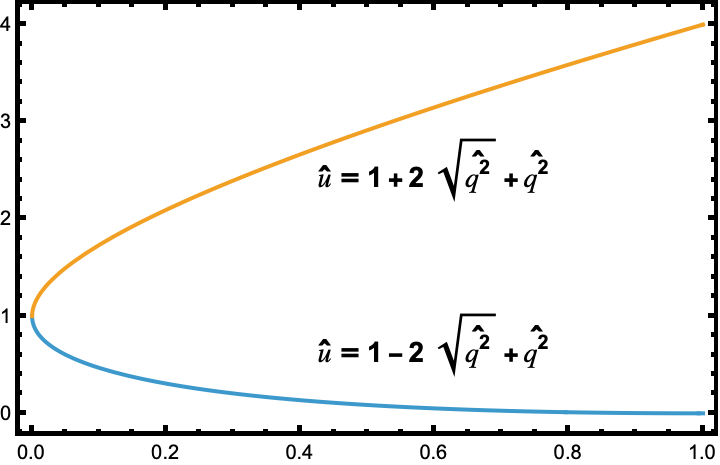
\includegraphics[width=\linewidth]{figures/singR1.png}
        \caption{实发射部分奇点分析1}
        \label{fig:sing_R1}
    \end{minipage}\hfill
    \begin{minipage}{0.5\textwidth}
        \centering
        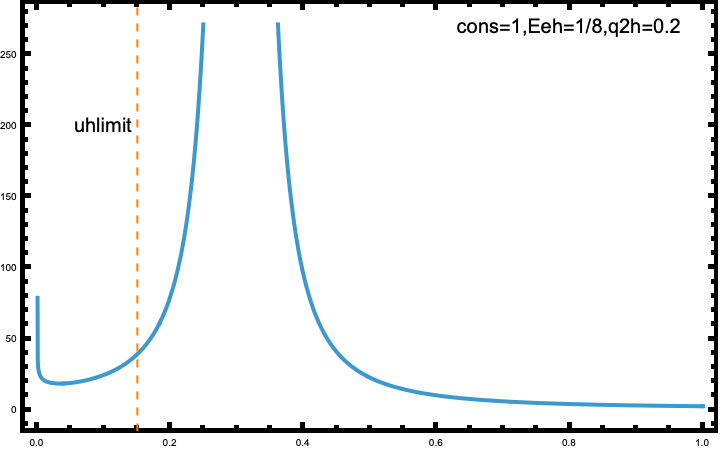
\includegraphics[width=\linewidth]{figures/singR2.png}
        \caption{实发射部分奇点分析2}
        \label{fig:sing_R2}
    \end{minipage}
\end{figure}
由于$\hat{u}$的物理区域是$\left[0,1\right]$，因此橙色曲线对应的奇点分布是非物理的。至于蓝色曲线对应的奇点分布，如图\ref{fig:sing_R2}所示，其中橙色虚线表示$\hat{u}$的积分上限，图中的发散区域对应于图\ref{fig:sing_R1}上$\hat{q^{2}}=0.25$附近，结果表明物理的奇点不在$\hat{u}$的积分区域以内。因此，式\eqref{eq:r_example}在$\hat{u}$的积分区域内不存在关于$\hat{u}$的不可积奇点。
\paragraph{B函数的相关项} 将三部分中的$B(\hat{u},{\hat{q^{2}}})$相关的项放在一起进行积分，其中最「奇异」的部分为：
    \begin{equation}
        \frac{2\left(2 \hat{E}_{\mathrm{e}}-\hat{q}^2-1\right)}{\hat{u}}\left[\left(2 \hat{E}_{\mathrm{e}}-\hat{q}^2\right) \mathcal{L}_2-\frac{\left(\hat{q}^2-1\right)\left(\hat{q}^2-2 \hat{E}_{\mathrm{e}}\right) \mathcal{L}_1}{\Delta}\right]
        \label{eq:B_example}
    \end{equation}
其中，$\Delta=\sqrt{\left(-\hat{q}^2+\hat{u}+1\right)^2-4 \hat{u}}$,$\mathcal{L}_1=\log \left(\frac{\Delta-\hat{q}^2+\hat{u}+1}{-\Delta-\hat{q}^2+\hat{u}+1}\right)$,$\mathcal{L}_2=\log \left(\frac{\hat{u}}{\left(\hat{q}^2-1\right)^2}\right)$。 式\eqref{eq:B_example}中似乎表明被积函数在$\hat{u}=0$处发散，对被积函数在$\hat{u}=0$处进行泰勒展开\footnote{泰勒展开的领头阶事实上对应于$\hat{u}$趋于零的极限}并分析发散行为\footnote{确定正规化参数取极限的方向以及积分限的偏移方向是必要的，否则会引入新的发散或错误，特别地，需要谨慎积分变量换元之后积分限的偏移方向。}是必要的。基于量子场论正规化思想，引入正规化常数$\epsilon$至积分区域边界处：
\begin{equation}
    \int_{0}^{1} f(\hat{u}) \mrm{d}\hat{u}\rightarrow\int_{\epsilon}^{1} f(\hat{u}) \mrm{d}\hat{u}\quad\quad \mrm{Im}(\epsilon)=0\text{且}\epsilon>0.
\end{equation}
积分完成后，取正规化参数趋于零的极限，结果表明式\eqref{eq:B_example}存在一个有限的积分结果。
\subsection{单圈水平上$\mrm{D\to X e^{+}\nu}$过程的领先幂次修正}
结合粲强子半轻单举衰变与底强子半轻单举衰变的区别，可得粲强子半轻单举衰变的电子能谱中对应于单圈水平上领先幂次修正的部分，电子能谱在电子能量的端点区域具有对数发散(可积发散)。对其进行加权积分，可得各类物理观测量的解析形式。

事实上，$\mrm{D\to X e^{+}\nu}$主要包含两个过程，分别是$\mrm{D\to X_s e^{+}}$和$\mrm{D\to X_d e^{+}\nu}$。对于前者，由于奇异夸克质量并非特别小，这里作为一个软自由度进行保留，有关末态有限夸克质量效应的修正，本文采用了Mannel等人\ct{Fael:2019umf}的工作。$\mrm{D\to X e^{+}\nu}$的衰变宽度为：
对于衰变宽度，
\begin{equation}
\begin{aligned}
    \Gamma_{D_{i}} = \sum_{q = \mathrm{d}, \mathrm{s}} \hat{\Gamma}_0 \mrm{\left| V_{\mathrm{c}q} \right|^2} m_{\mathrm{c}}^5 \Big\{ 1 & + \frac{\alpha_s}{\pi} \frac{2}{3} \left( \frac{25}{4} - \pi^2 \right)\\
    & + \frac{\alpha_s^2}{\pi^2} \left[ \frac{\beta_0}{4} \frac{2}{3} \left( \frac{25}{4} - \pi^2 \right) \log \left( \frac{\mu^2}{m_{\mathrm{c}}^2} \right) + 2.14690 n_l - 29.88311 \right]\\  
    &- 8 \rho \delta_{\mathrm{s}q} - \frac{1}{2} \frac{\mu_{\pi}^{2}(D_{i})}{m_{\mathrm{c}}^2} - \frac{3}{2} \frac{\mu_{\mathrm{G}}^{2}(D_{i})}{m_{\mathrm{c}}^2} + 6 \frac{\rho_{\mathrm{D}}^3\left(D_{i}\right)}{m_{\mathrm{c}}^3} + \dots \Big\},
\end{aligned}
\label{eq:decaywidth}
\end{equation}
式\eqref{eq:decaywidth}中，$\hat{\Gamma}_0 = {G_F^2 }/{(192 \pi^3)}$, $V_{cq}$ 是对应过程的CKM矩阵元，指标$i=u, d, s$分别指$\mrm{D^{+}}$,$\mrm{D^{0}}$和$\mrm{D_s^+}$, $\beta_0 = 11-2n_f /3$是量子色动力学$\beta$函数的第一个系数, $\rho\equiv m_s^2/m_c^2$. 对于微扰修正，$n_{f}=4$对应于$n_{l}=3$。本文微扰部分的单圈修正结果与DeFazio，Capdevila等人的工作一致\cite{DeFazio:1999ptt,Capdevila:2021vkf}. VanRitbergen和Brucherseifer等人讨论了$\mrm{b\to u}$过程的两圈图水平上领先幂次的修正，在衰变宽度的意义上，底强子弱衰变弱衰变$n_{f}=5$而粲强子单举弱衰变的$n_{f}=4$。本文关于两圈图修正的数值结果由陈龙、马滟青老师提供。
关于\ref{eq:decaywidth}中非微扰矩阵元的定义，本文采用Mannel等人的约定\ct{Fael:2019umf}：
\begin{equation}
    \begin{aligned}
        \mu_\pi^2(D_i) &\equiv \langle D_i| \bar c_v(iD)^2 c_v| D_i \rangle /(2m_{D_i}) , \; \\
        \mu_G^2(D_i) &\equiv \langle D_i| \bar c_v (iD_\alpha)(iD_\beta)(-i\sigma^{\alpha\beta}) c_v| D_i \rangle  /(2m_{D_i}),  \\
        \rho_{LS}^3(D_i) &\equiv {1\over2}\langle D_i| \bar c_v \{(iD_\alpha), [iv\cdot D, iD_\beta ]\} (-i\sigma^{\alpha\beta})| D_i \rangle /(2m_{D_i}) , \;\\ 
        \rho^3_{D}(D_i) &\equiv {1\over2}\langle D_i| \bar c_v  [(iD^\mu), [iv\cdot D, iD_\mu]] c_v | D_i \rangle /(2m_{D_i}). \; \\
        \end{aligned}
\end{equation}
      n阶电子能量原点矩，其定义如下
      \begin{equation}
        \langle E_{\mathrm{e}}^{n} \rangle = \frac{1}{\Gamma} \int \hat{E}_{\mathrm{e}}^{n} \frac{d \Gamma}{d \hat{E}_{\mathrm{e}}} \, d \hat{E}_{\mathrm{e}},
\end{equation}
      其中， $\Gamma$是衰变宽度，$n=1, 2, 3\cdots$.
      对电子能谱进行加权积分，前四阶电子能量（原点）矩.
      如下所示，
      \begin{equation}
        \scriptsize
        \begin{aligned}
            \langle E_{e}\rangle_{D_{i}}&=\frac{\hat{\Gamma}_0}{    \Gamma_{D_{i}}}\sum_{q=d,s} \left|V_{cq}\right|^2 m_{c}^6 \left[\frac{3}{10} + \frac{\alpha_{s}}{\pi} a_1^{(1)} + {\alpha_s^2\over \pi^2}a_1^{(2)} -3\rho\delta_{sq} -\frac{1}{2}\frac{\mu_{G}^{2}(D_{i})}{m_{c}^{2}} +\frac{139}{30} \frac{\rho_D^3\left(D_{i}\right)}{m_c^3}+\frac{3}{10} \frac{\rho_{L S}^3\left(D_{i}\right)}{m_c^3}+ ...\right],\\
            \langle E_{e}^{2} \rangle_{D_{i}} &=\frac{\hat{\Gamma}_0}{\Gamma_{D_{i}}} \sum_{q=d,s}\left|V_{cq}\right|^2 m_c^7 \left[ \frac{1}{10} + \frac{\alpha_{s}}{\pi} a_2^{(1)}  + {\alpha_s^2\over \pi^2}a_2^{(2)}  - \frac{6}{5} \rho\delta_{sq} + \frac{1}{12}\frac{\mu_{\pi}^2(D_{i})}{ m_c^2} - \frac{11}{60}\frac{\mu_G^2(D_{i})}{ m_c^2} +\frac{17}{6} \frac{\rho_D^3\left(D_{i}\right)}{m_c^3} \right.\nonumber \\
            &\qquad\qquad\qquad\qquad\qquad \left. +\frac{7}{30} \frac{\rho_{L S}^3\left(D_{i}\right)}{m_c^3}+ ... \right], \nonumber\\
            \left\langle E_e^3\right\rangle_{D_{i}}&=\frac{\hat{\Gamma}_0}{\Gamma_{D_{i}}}\sum_{q=d,s}\left|V_{cq}\right|^2 m_c^8\left[\frac{1}{28} + \frac{\alpha_{s}}{\pi} a_3^{(1)}  + {\alpha_s^2\over \pi^2}a_3^{(2)}  -\frac{1}{2} \rho\delta_{sq} +\frac{1}{14} \frac{\mu_\pi^2\left(D_{i}\right)}{ m_c^2}-\frac{1}{14} \frac{\mu_G^2\left(D_{i}\right)}{ m_c^2}+\frac{223}{140} \frac{\rho_D^3\left(D_{i}\right)}{m_c^3}\right. \nonumber\\
            &\qquad\qquad\qquad\qquad\qquad \left.+\frac{1}{7} \frac{\rho_{L S}^3\left(D_{i}\right)}{m_c^3} + ... \right],\nonumber\\
            \left\langle E_e^4\right\rangle_{D_i}&=\frac{\hat{\Gamma}_0}{\Gamma_{D_{i}}}\sum_{q=d,s}\left|V_{cq}\right|^2 m_c^9\left[\frac{3}{224} + \frac{\alpha_{s}}{\pi} a_4^{(1)}  + {\alpha_s^2\over \pi^2}a_4^{(2)}  -\frac{3}{14} \rho\delta_{sq} +\frac{3}{64} \frac{\mu_\pi^2\left(D_{i}\right)}{ m_c^2}-\frac{13}{448} \frac{\mu_G^2\left(D_{i}\right)}{ m_c^2} +\frac{481}{560} \frac{\rho_D^3\left(D_i\right)}{m_c^3}\right. \nonumber\\
            &\qquad\qquad\qquad\qquad\qquad \left.+\frac{9}{112} \frac{\rho_{L S}^3\left(D_i\right)}{m_c^3}+ ... \right],\nonumber
            \end{aligned}
            \label{eq:inital_moments}
      \end{equation}
      式\eqref{eq:inital_moments}的NLO和NNLO系数如下所示，
      \begin{equation}
        \scriptsize
      \begin{aligned}
        a^{(1)}_1 &= {1093 - 180\pi^2\over 900 }, \;
        a^{(1)}_2 = \frac{4243 - 720 \pi^2}{{10800}}, \; 
        a^{(1)}_3 = \frac{144037-25200 \pi^2}{{1058400}}, \; 
        a^{(1)}_4 = \frac{69827-12600 \pi^2}{{1411200}},   \\
        a^{(2)}_1 &= {\beta_0\over 4}a^{(1)}_1\ell -7.70077, \; 
        a^{(2)}_2 = {\beta_0\over 4}a^{(1)}_2\ell -2.77835, \; 
        a^{(2)}_3 = {\beta_0\over 4}a^{(1)}_3\ell -1.06371 , \; 
        a^{(2)}_4 = {\beta_0\over 4}a^{(1)}_4\ell -0.42438 , \nonumber
        \end{aligned}
    \end{equation}
        本文关于前两阶电子能量（原点）矩的结果与Kamenik等人的工作\cite{Kamenik:2011zz}一致，树图水平上量纲六算符的修正来源于Mannel等人的工作\cite{Fael:2019umf}，前四阶矩的领头阶与Mannel等人的结果\cite{Fael:2019umf}一致。
        事实上，本文同样提供了电子能量第二、三、四阶的中心矩，电子能量的中心矩由原点矩线性组合而成，定义如下：
        \begin{equation}
            \scriptsize
        \begin{aligned}
            \left\langle E_e\right\rangle, \;\left\langle E_e^2\right\rangle_{\rm center}\equiv \left\langle (E_e - \langle E_e\rangle)^2 \right\rangle , \; \left\langle E_e^3\right\rangle_{\rm center}\equiv\left\langle (E_e - \langle E_e\rangle)^3 \right\rangle , \; \left\langle E_e^4\right\rangle_{\rm center}\equiv\left\langle (E_e - \langle E_e\rangle)^4 \right\rangle .
            \end{aligned}
        \end{equation}
    由于物理可观测量对粲夸克质量的高度敏感性，有关粲夸克质量方案的讨论是必要的，具体讨论将在第四章全局拟合的部分呈现。
\section{更高量纲算符非微扰矩阵元的参数化}
上一节通过对电子能谱的加权积分得到各类物理可观测量，其中量纲六算符非微扰矩阵元的贡献来自于Mannel等人的工作\ct{Fael:2019umf}。本节基于Lenz等人的工作\ct{King:2021jsq}对量纲六算符非微扰矩阵元的参数化进行简单介绍。

量纲六算符分为两夸克算符和四夸克算符，对于两夸克算符，仅$\rho_{D}^{3}$对衰变宽度由贡献，其非微扰矩阵元可做如下的参数化
\begin{equation}
    2 m_D \rho_D^3(D)=\langle D(p)| \bar{c}_v\left(i D_\mu\right)(i v \cdot D)\left(i D^\mu\right) c_v|D(p)\rangle .
    \end{equation}
    在衰变宽度的水平上，
    \begin{equation}
        \Gamma_6 \frac{\left\langle\mathcal{O}_6\right\rangle}{m_c^3}=\Gamma_0 c_{\rho_D} \frac{\rho_D^3}{m_c^3}
        \end{equation}
    其中,$\Gamma_{0}=\frac{G_F^2 m_c^5 V_{\text{CKM}}}{192\pi^3}$, $c_{\rho_D}=3 C_1^2 \mathcal{C}_{\rho_D, 11}+2 C_1 C_2 \mathcal{C}_{\rho_D, 12}+3 C_2^2 \mathcal{C}_{\rho_D, 22}+\mathcal{C}_{\rho_D, \mrm{S L}}$.

    对于底强子弱衰变过程，Lenz，Mannel和Daniel等人的工作\ct{Lenz:2020oce,Mannel:2020fts,Moreno:2020rmk}给出了非轻部分的Wilson系数，其中需要处理来自轻自由度的软胶子辐射，会导致$\ln(m_{q}/m_{b})$的对数发散，事实上，将四夸克算符以及算符混合的贡献考虑在内，则可以完全消除； 对于底强子的半轻衰变，由于$\rho=m_\mrm{c}^2/m_\mrm{b}^2$不是一个小量，$\mrm{b\to c e\nu_e}$过程量纲六算符的Wilson系数是有限的，但中间无质量传播子发射软胶子使得$b\to u e\nu $过程量纲六算符对应的Wilson系数存在发散。
    
    对于粲强子弱衰变过程，由于，$m_{\mrm{c}}>>m_{s}\sim \Lambda_{QCD}$，因此末态奇异夸克质量作为软自由度与四夸克算符的混合需要额外考虑， Lenz等人的工作\ct{King:2021xqp}讨论了这部分的Wilson系数，并将其用于D介子寿命的理论计算。
    
    量纲六算符中四夸克算符来源于旁观者夸克效应，存在以下三种贡献(图\ref{fig:spector})，
    \begin{figure}[h!]
        \centering
        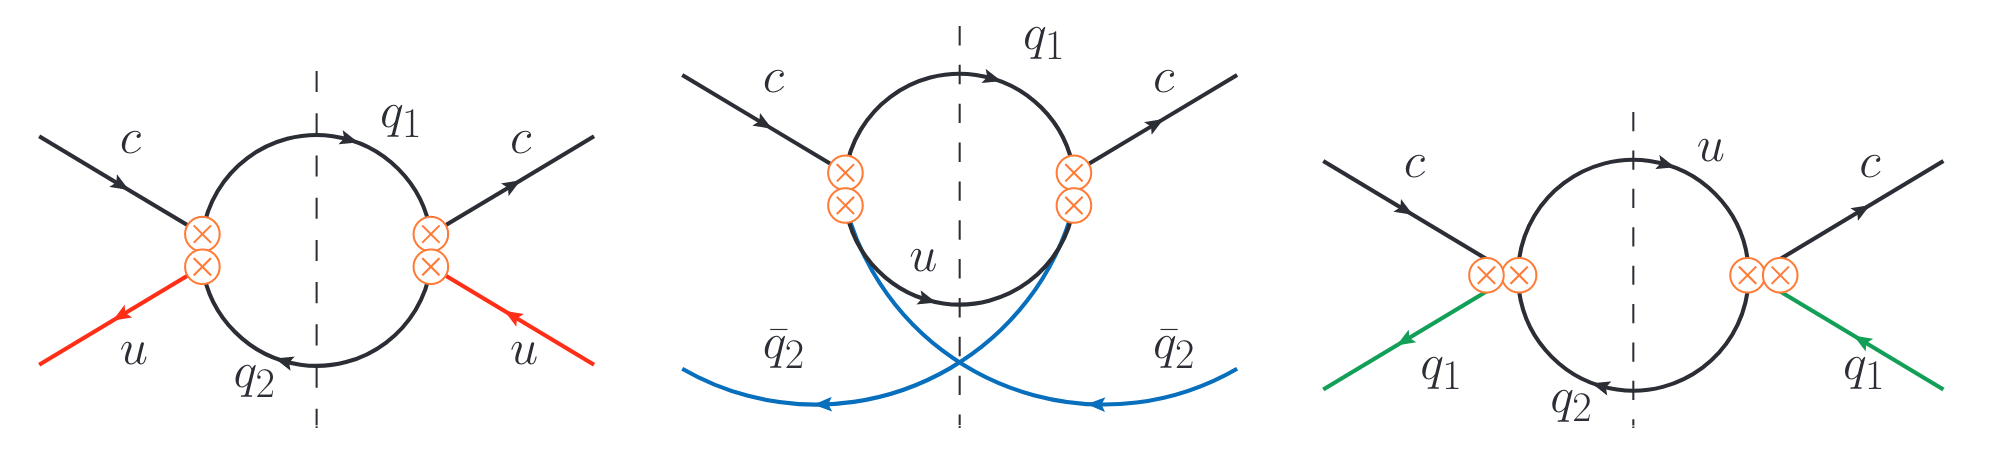
\includegraphics[width=\textwidth]{figures/spector.png}
        \caption{重夸克展开的旁观者夸克效应拓扑图\ct{King:2021xqp}}
        \label{fig:spector}
    \end{figure}
图\ref{fig:spector}中从左至右分别是弱交换（Weak Exchange， WE）、泡利干涉（Pauli Interference，PI）和弱湮灭（Weak Annihilation，WA）贡献\footnote{半轻衰变只存在弱湮灭贡献}。量纲六算符中的四夸克算符如下所示\footnote{两个等号表示存在两种记号}
\begin{equation}
    \begin{aligned}
    & O_1^q=\left(\bar{c} \gamma_\mu\left(1-\gamma_5\right) q\right)\left(\bar{q} \gamma^\mu\left(1-\gamma_5\right) c\right), \\
    & O_2^q=\left(\bar{c}\left(1-\gamma_5\right) q\right)\left(\bar{q}\left(1+\gamma_5\right) c\right), \\
    & O_3^q=T_1^q=\left(\bar{c} \gamma_\mu\left(1-\gamma_5\right) T^A q\right)\left(\bar{q} \gamma^\mu\left(1-\gamma_5\right) T^A c\right), \\
    & O_4^q=T_2^q=\left(\bar{c}\left(1-\gamma_5\right) T^A q\right)\left(\bar{q}\left(1+\gamma_5\right) T^A c\right),
    \end{aligned}
    \end{equation}
在量子色动力学框架下，其非微扰矩阵元进行如下的参数化，
\begin{equation}
    \begin{aligned}
    \left\langle D_q\right| O_i^q\left|D_q\right\rangle & =A_i f_{D_q}^2 m_{D_q}^2 B_i^q \\
    \left\langle D_q\right| O_i^{q^{\prime}}\left|D_q\right\rangle & =A_i f_{D_q}^2 m_{D_q}^2 \delta_i^{q q^{\prime}}, \quad q \neq q^{\prime}
    \end{aligned}
    \end{equation}
    其中，$A_1^q=A_3^q=1, \quad A_2^q=A_4^q=\frac{m_D^2}{\left(m_c+m_q\right)^2}$，$f^2_{D_{q}}$量子色动力学框架下的$D_{q}$介子的衰变常数，$m_{D_{q}}$是$D_{q}$质量，$B_{i}^{q}$是Bag 参数。
在重夸克有效理论框架下，量纲六算符中的四夸克算符为：
\begin{equation}
    \begin{aligned}
    & \tilde{O}_1^q=\left(\bar{h}_v \gamma_\mu\left(1-\gamma_5\right) q\right)\left(\bar{q} \gamma^\mu\left(1-\gamma_5\right) h_v\right), \\
    & \tilde{O}_2^q=\left(\bar{h}_v\left(1-\gamma_5\right) q\right)\left(\bar{q}\left(1+\gamma_5\right) h_v\right), \\
    & \tilde{O}_3^q=\tilde{T}_1^q=\left(\bar{h}_v \gamma_\mu\left(1-\gamma_5\right) T^A q\right)\left(\bar{q} \gamma^\mu\left(1-\gamma_5\right) T^A h_v\right), \\
    & \tilde{O}_4^q=\tilde{T}_2^q=\left(\bar{h}_v\left(1-\gamma_5\right) T^A q\right)\left(\bar{q}\left(1+\gamma_5\right) T^A h_v\right),
    \end{aligned}
    \end{equation}
其中$h_{v}$是积掉重自由度的有效重夸克场，量纲六算符中的四夸克算符可以进行如下的参数化，
\begin{equation}
    \begin{aligned}
    \left\langle D_q\right| \tilde{O}_i^q\left|D_q\right\rangle & =F^2(\mu) m_{D_q} \tilde{B}_i^q \\
    \left\langle D_q\right| \tilde{O}_i^{q^{\prime}}\left|D_q\right\rangle & =F^2(\mu) m_{D_q} \tilde{\delta}_i^{q^{\prime} q}, \quad q \neq q^{\prime},
    \end{aligned}
    \label{eq:dim6_4_parameters}
    \end{equation}
    其中$q, q^{\prime}=u, d, s, \tilde{B}_i^q$表示HQET中的Bag参数，$\tilde{B}_{1,2}^q$对应于色单态算符，$\tilde{B}_{3,4}^q \equiv \tilde{\epsilon}_{1,2}^q$对应于色八态算符，$F(\mu)$是HQET衰变常数。
    \begin{equation}
        \begin{aligned}
            \langle 0| \bar{q} \gamma^\mu \gamma_5 h_v\left|D_q(v)\right\rangle_{\mathrm{HQET}}&=i F(\mu) \sqrt{m_{D_q}} v^\mu,\\
            \langle 0| \bar{q} \gamma^\mu \gamma_5 c\left|D_q(p)\right\rangle_{\mathrm{QCD}}&=i f_{D_q} p^\mu
        \end{aligned}
        \end{equation}
    \paragraph{真空插入近似假设(vacuum insertion approximation, VIA)}为简化强子内部相互作用，近似假设强子内为真空态，其色场被近似为色单态。具体地，在四夸克算符矩阵元中插入一组完备集，仅保留真空态贡献，将四夸克算符非微扰矩阵元因子化为衰变常数和Bag参数的乘积，Bag参数依赖于算符中的色结构。
    色单态算符对应的Bag参数为假设为1， 色八重态算符对应的Bag参数被假设为0。

    式\eqref{eq:dim6_4_parameters}中的$\tilde{\delta}_i^{q^{\prime} q}$描述了eye-contractions,如图\ref{fig:eye}所示，eye-contractions指由于内外夸克之间的相互作用，它们以一种特定的方式被连接起来。
    \begin{figure}[h!]
        \centering
        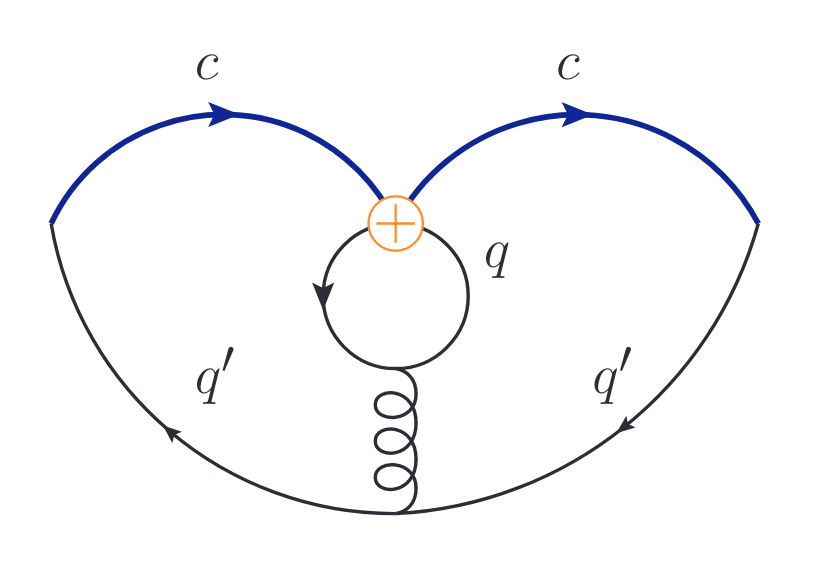
\includegraphics[width=0.4\textwidth]{figures/eye.png}
        \caption{量纲六算符非微扰矩阵元之一：Eye-contractions 效应\ct{King:2021xqp}}
        \label{fig:eye}
    \end{figure}
     
    受到$\alpha_s$的压低，真空插入近似下，Eye-contractions贡献被假设为零。在重夸克有效理论求和规则中（Heavy Quark Effective Theory Sum Rule, HQETSR），表征Eye-contractions的参数$\tilde{\delta}_i^{q^{\prime} q}$则并不严格为零。
    \begin{table}[h!]
        \centering
        \small % 或 \footnotesize 进一步缩小
        \setlength{\tabcolsep}{4pt} % 减少列间距
        \renewcommand{\arraystretch}{1.1} % 微调行高
        \begin{tabular}{|c||c|c|c|c|}
            \hline 
            HQET, $\mu_0=1.5 \mathrm{GeV}$ & $\tilde{B}_1$ & $\tilde{B}_2$ & $\tilde{\epsilon}_1$ & $\tilde{\epsilon}_2$ \\
            \hline
            $D^{+, 0}$ & $1.0026_{-0.0106}^{+0.0198}$ & $0.9982_{-0.0066}^{+0.0052}$ & $-0.0165_{-0.0346}^{+0.0209}$ & $-0.0004_{-0.0326}^{+0.0200}$ \\
            \hline
            $D_s^{+}$ & $1.0022_{-0.0099}^{+0.0185}$ & $0.9983_{-0.0067}^{+0.0052}$ & $-0.0104_{-0.0330}^{+0.0202}$ & $0.0001_{-0.0324}^{+0.0199}$ \\
            \hline \hline 
            HQET, $\mu_0=1.5 \mathrm{GeV}$ & $\tilde{\delta}_1$ & $\tilde{\delta}_2$ & $\tilde{\delta}_3$ & $\tilde{\delta}_4$ \\
            \hline
            $\left\langle D_q\right| \tilde{O}^q\left|D_q\right\rangle$ & $0.0026_{-0.0092}^{+0.0142}$ & $-0.0018_{-0.0072}^{+0.0047}$ & $-0.0004_{-0.0024}^{+0.0015}$ & $0.0003_{-0.0008}^{+0.0012}$ \\
            \hline
            $\left\langle D_s\right| \tilde{O}^q\left|D_s\right\rangle$ & $0.0025_{-0.0093}^{+0.014}$ & $-0.0018_{-0.0072}^{+0.0047}$ & $-0.0004_{-0.0024}^{+0.0015}$ & $0.0003_{-0.0008}^{+0.0012}$ \\
            \hline
            $\left\langle D_q\right| \tilde{O}^s\left|D_q\right\rangle$ & $0.0023_{-0.0091}^{+0.0140}$ & $-0.0017_{-0.0070}^{+0.0046}$ & $-0.0004_{-0.0023}^{+0.0015}$ & $0.0003_{-0.0008}^{+0.0012}$ \\
            \hline
        \end{tabular}
        \caption{HQETSR关于Bag参数的数值结果}
        \label{tab:HQETSR_num_Bag}
    \end{table}
    值得注意的是，\(\mrm{ D^{+, 0}} \) 介子的 Bag 参数 \( \tilde{B}_i^q \) 的HQETSR的预言由Lenz等人的工作\ct{Kirk:2017juj}给出,同时他们也给出了Eye-contractions效应的HQETSR的预言\ct{King:2021jsq}。如表\ref{tab:HQETSR_num_Bag}所示，
基于真空插入近似，表征Eye-contractions效应的参数和色八重态算符对应的Bag参数被假设为零，色单态算符非微扰矩阵元收到相应Wilson系数压低，这是我们从实验数据中抽取量纲五算符和量纲六算符两夸克算符非微扰矩阵元的理论依据。
\section{本章回顾}
基于第二章关于重夸克有效理论和算符乘积简单介绍，深入介绍了本文理论方面的努力。首先基于Mark.B.Wise的经典教材\ct{manohar2000heavy}介绍了$\mrm{\mrm{B}\to X_{c}e\nu}$过程Wilson系数的匹配和末态相空间的解析积分,获得该过程以及$\mrm{\mrm{B}\to X_{u}e\nu}$过程电子能谱的解析形式；其次，基于更现代的运动学变量对$\mrm{\mrm{B}\to X_{c}e\nu}$过程进行相同的讨论，并给出两组运动学变量（运动学参数化方案）之间的联系；此外，基于更现代的运动学变量对$\mrm{\mrm{B}\to X_{c}e\nu}$过程领先幂次修正的单圈微扰修正进行讨论，并推广至$\mrm{\mrm{B}\to X_{u}e\nu}$过程；最后，本章将有关B介子半轻单举衰变的讨论转换到$\mrm{D\to X e^{+}\nu}$过程，对电子能谱进行加权积分，获得了衰变宽度、电子能量一、二、三、四阶原点矩。以上的讨论为D介子半轻单举衰变的系统性唯象学分析奠定了理论基础。
\chapter{粲介子半轻单举衰变的数据处理与唯象学分析}
本章将系统性讨论D介子半轻单举衰变的唯象学分析。首先，对我国高能物理研究所的BESIII合作组和美国康奈尔大学的CLEO合作组测量$\mrm{D}$介子半轻单举衰变的实验现状进行介绍并讨论相关物理可观测量的抽取。其次，由于衰变宽度对重夸克质量高度敏感，本文将讨论三种不同的重夸克质量机制，分别是1S mass，$\overline{\mathrm{MS}}$ mass scheme和Pole mass scheme。对于唯象学分析，本文在三种质量方案下对非微扰参数进行了两种情形的全局拟合估计，分别是包含量纲三算符和五算符矩阵元贡献与包含量纲三算符，量纲五算符量纲六算符矩阵元贡献，并就非微扰参数的拟合估计结果进行讨论。最后定性讨论非微扰参数的拟合估计值对D介子寿命的影响。
\section{实验现状}
\subsection{D介子半轻单举衰变绝对分支比的实验测量}
CLEO合作组于2009年对三种$\mrm{D}$介子半轻衰变进行了测量\ct{CLEO:2009uah}。他们利用$e^{+}e^{-}$对撞，在质心能量$\mrm{E_{\mrm{cm}}}=3.774 \GeV$处积累了$818 \mathrm{pb}^{-1}$的$\mrm{D^{0}\overline{D^{0}}}$和$\mrm{D^{+} D^{-}}$事例，并测量了实验系下电子能谱$(\mrm{p_{e}>0.2\GeV})$和衰变分支比。此外，基于已知的遍举衰变数据对电子能谱$(\mrm{p_{e}>0.2\GeV})$进行红外端的外推，以测量$\mrm{D^{0}\to X e^{+}\nu}$和$\mrm{D^{+}\to X e^{+}\nu}$两个过程的电子能谱。对于$\mrm{D_s^+}$介子，他们在质心能量$\mrm{E_{\mrm{EM}}=4.170\GeV}$处积累了$602 \mrm{pb^{-1}}$的$\mrm{D_s^{*\pm}\mrm{D_s}^{\mp}}$事例，对$\mrm{D_s^{+}\to X e^{+}\nu}$的衰变分支比和电子能谱$(\mrm{p_{e}>0.2\GeV})$进行测量。并基于已知遍举衰变数据实现电子能谱的红外端外推，以获得该过程的电子能谱。CLEO合作组的测量结果为：

\begin{equation}
    \begin{aligned}
        \mathcal{B}\left(\mrm{D^0 \rightarrow X e^{+} \nu_e}\right)&=(6.46 \pm 0.09 \pm 0.11) \%,\\
        \mathcal{B}\left(\mrm{D^{+} \rightarrow X e^{+} \nu_e}\right)&=(16.13 \pm 0.10 \pm 0.29) \%,\\
        \mathcal{B}\left(\mrm{D_s^{+} \rightarrow X e^{+} \nu_e}\right)&=(6.52 \pm 0.39 \pm 0.15) \%,\\
    \end{aligned}
    \label{eq:CLEOBr}
\end{equation}
其中，两个误差分别是统计误差和系统误差。此外，他们讨论了D介子半轻单举过程$\mrm{SU(3)}$味道对称性的破坏，
$$
\begin{aligned}
    \Gamma\left(D^{+} \rightarrow X e^{+} \nu_e\right) / \Gamma\left(D^0 \rightarrow X e^{+} \nu_e\right)&=0.985 \pm 0.015 \pm 0.024,\\
    \Gamma\left(D_s^{+} \rightarrow X e^{+} \nu_e\right) / \Gamma\left(D^0 \rightarrow X e^{+} \nu_e\right)&=0.828 \pm 0.051 \pm 0.025,
\end{aligned}
$$
与理论预期基本相符。
\begin{figure}[htbp]
    \centering
    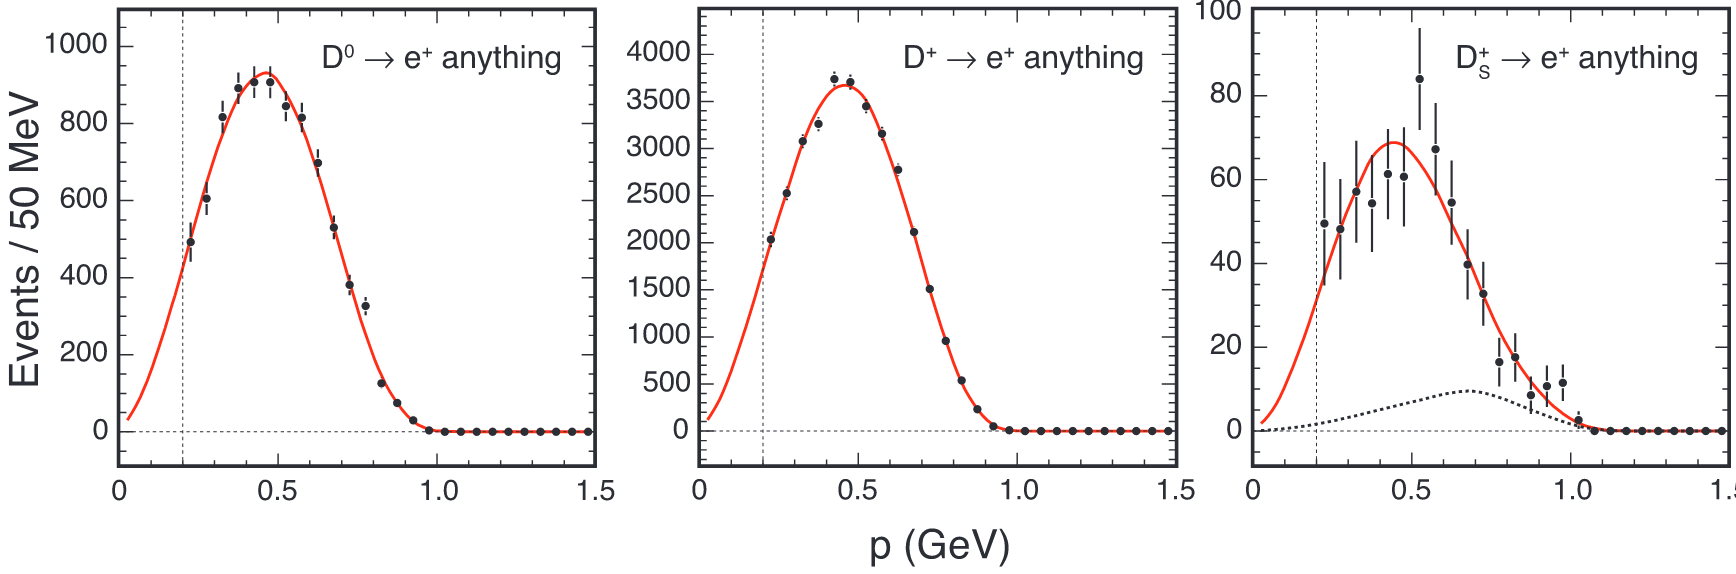
\includegraphics[width=1\textwidth]{figures/CLEOElectronsppart.png}
    \caption{实验室系下$\mrm{D}\to X e^+\nu$衰变过程的电子能谱\ct{CLEO:2009uah}}$\left(\mrm{p_{e}}> 0.2\GeV\right)$ % 添加图例
    \label{fig:cleo}  % 添加标签
\end{figure}
图\ref{fig:cleo}是CLEO合作组对$\mrm{D\to X e^+\nu}$过程电子能谱的测量结果,其中灰色垂直线表明电子的识别动量被截断于$0.2\GeV$处，误差棒仅包含统计误差。基于已知遍举衰变数据，红色实线是电子能谱的拟合结果。CLEO合作组提供了图\ref{fig:cleo}中对应每个bin的具体事例数和对应的统计误差，如表\ref{tab:cleo_electron_sp}所示，对于 $\mrm{D^{+}}$ 和 $\mrm{D_s^{+}}$，已经减除了来自轻子衰变 $\tau^{+} \nu_\tau$（ $\tau^{+} \rightarrow e^{+} \nu_e \bar{\nu}_\tau$）的贡献。结果表明 $\mrm{D^{0}}$与$\mrm{D^{+}}$介子的衰变电子能谱具有较高精度，但$\mrm{D_s^{+}}$介子的衰变电子能谱的精度较低。我国BESIII合作组于2021年重新抽取$\mrm{D_s^{+}}$介子的衰变电子能谱\ct{BESIII:2021duu}。
\begin{table}[h!]
    \centering
    \scriptsize  % 设置表格字体为小号
    \begin{tabular}{lrrr}
        \hline \hline
        $p(\mathrm{GeV})$ & $\Delta B\left(D^0 \rightarrow X e^{+} \nu_e\right)(\%)$ & $\Delta B\left(D^{+} \rightarrow X e^{+} \nu_e\right)(\%)$ & $\Delta B\left(D_s^{+} \rightarrow X e^{+} \nu_e\right)(\%)$ \\
        \hline 
        $0.200-0.250$ & $0.347 \pm 0.036$ & $0.912 \pm 0.040$ & $0.491 \pm 0.152$ \\
        $0.250-0.300$ & $0.426 \pm 0.030$ & $1.133 \pm 0.038$ & $0.470 \pm 0.124$ \\
        $0.300-0.350$ & $0.576 \pm 0.031$ & $1.379 \pm 0.041$ & $0.554 \pm 0.126$ \\
        $0.350-0.400$ & $0.629 \pm 0.030$ & $1.462 \pm 0.043$ & $0.515 \pm 0.120$ \\
        $0.400-0.450$ & $0.640 \pm 0.031$ & $1.675 \pm 0.047$ & $0.578 \pm 0.112$ \\
        $0.450-0.500$ & $0.640 \pm 0.031$ & $1.661 \pm 0.046$ & $0.562 \pm 0.123$ \\
        $0.500-0.550$ & $0.596 \pm 0.029$ & $1.546 \pm 0.044$ & $0.794 \pm 0.127$ \\
        $0.550-0.600$ & $0.575 \pm 0.029$ & $1.415 \pm 0.041$ & $0.611 \pm 0.115$ \\
        $0.600-0.650$ & $0.492 \pm 0.026$ & $1.243 \pm 0.038$ & $0.471 \pm 0.104$ \\
        $0.650-0.700$ & $0.374 \pm 0.023$ & $0.946 \pm 0.032$ & $0.314 \pm 0.087$ \\
        $0.700-0.750$ & $0.269 \pm 0.019$ & $0.674 \pm 0.026$ & $0.246 \pm 0.079$ \\
        $0.750-0.800$ & $0.230 \pm 0.017$ & $0.429 \pm 0.019$ & $0.089 \pm 0.060$ \\
        $0.800-0.850$ & $0.089 \pm 0.011$ & $0.240 \pm 0.014$ & $0.115 \pm 0.060$ \\
        $0.850-0.900$ & $0.053 \pm 0.008$ & $0.103 \pm 0.009$ & $0.037 \pm 0.046$ \\
        $0.900-0.950$ & $0.021 \pm 0.005$ & $0.022 \pm 0.004$ & $0.074 \pm 0.051$ \\
        $0.950-1.000$ & $0.002 \pm 0.002$ & $0.004 \pm 0.002$ & $0.096 \pm 0.045$ \\
        $1.000-1.050$ & $\cdots$ & $\cdots$ & $0.015 \pm 0.022$ \\
        \hline \hline
    \end{tabular}
    \caption{在实验室系下D介子半轻单举衰变过程每个bin的部分分支比\ct{CLEO:2009uah}}
    \label{tab:cleo_electron_sp}
\end{table}

%在我们接下来的唯象学分析中，对于$D_s^{+}$介子的衰变电子能谱，我们将使用BESIII合作组的测量结果，并在此基础上进行可观测量的抽取；对于$D^{0}$与$D^{+}$介子的衰变电子能谱，我们使用CLEO合作组的测量结果。

\subsection{$\mrm{D_s^+}$介子半轻单举衰变绝对分支比的实验测量}

BESIII合作组近期对$\mrm{D_s^{+}}$介子半轻单举衰变分支比进行测量\cite{BESIII:2021duu}。他们采用双标记技术在BEPCII对撞机上质心能量$\mrm{E_{\text{cm}} \in [4.178, 4.230] \ \mathrm{GeV}}$处产生的$\mrm{e^{+} e^{-}}$湮灭事例进行分析。主要包括：
\begin{itemize}
\item 2016年，在质心能量$\mrm{E_{\mathrm{cm}}}=4.178 \, \text{GeV}$处产生了$3.19 \, \mathrm{fb}^{-1}$的事例，$\mrm{e^{+} e^{-} \rightarrow D_s^{*+} D_s^{-}}$产生了大约$6.4 \times 10^6$个$\mrm{D_s^{+}}$介子，以及少量来自$\mrm{e^{+} e^{-} \rightarrow D_s^{+} D_s^{-}}$的贡献
\item 2017年，在质心能量$\mrm{E_{\mathrm{cm}}}\in [4.189, 4.219]\GeV$处产生了$2.08 \, \mathrm{fb}^{-1}$的事例
\item 2013年，在质心能量$\mrm{E_{\mathrm{cm}}}\in [4.225, 4.230 ]\GeV$内收集的$1.05 \, \mathrm{fb}^{-1}$的事例
\end{itemize}

有关$\mrm{D_s^+}$半轻单举衰变绝对分支比和该过程$\mrm{SU(3)}$对称性破坏的测量结果为：
\begin{equation}
    \begin{aligned}
     \mathcal{B}\left(\mrm{D_s^{+} \rightarrow X e^{+} \nu_e}\right) 
    &=(6.30 \pm 0.13(\text { stat. }) \pm 0.09(\text { syst. }) \pm 0.04(\text { ext. })) \%,\\
         \frac{\Gamma\left(\mrm{D_s^{+} \rightarrow X e^{+} \nu_e}\right)}{\mrm{\Gamma\left(D^0 \rightarrow X e^{+} \nu_e\right)}} 
         &=0.790 \pm 0.016 \text { (stat.) } \pm 0.011 \text { (syst.) } \pm 0.016 \text { (ext.). }\\
    \end{aligned}
         \label{eq:BESIIIGamma__Br_Ds}  
        \end{equation}
式\eqref{eq:BESIIIGamma__Br_Ds}中的误差分别是统计误差，系统误差以及电子动量$\mrm{p_e<0.2\GeV}$区域的外推误差。该结果与CLEO合作组的测量结果基本一致，但BESIII合作组的测量精度更高。$\mrm{D_s}$介子半轻单举衰变宽度与$\mrm{D^0}$介子半轻单举衰变宽度的比值偏离1反映了$\mrm{SU(3)}$味道对称性的破坏。

此外，BESIII合作组基于已知遍举衰变数据对测量得到部分电子能谱进行红外端($\mrm{p}_{e}<0.2\GeV$的区域)外推，如图\ref{fig:BESIIIElectrons}所示，其中黑色带误差棒的点表示每个bin内的事例数，蓝色曲线表示拟合结果。结果表明，BESIII合作组的测量结果与CLEO合作组的测量结果基本一致。
\begin{figure}[htbp]
    \centering
    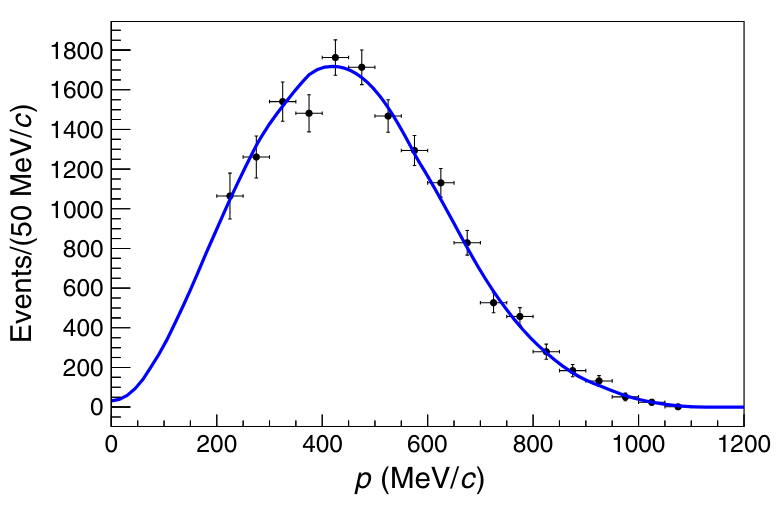
\includegraphics[width=0.6\textwidth]{figures/BESIIIElectrons.png}
    \caption{实验室系下$\mrm{D_s^+\to X e^+\nu}$衰变过程的电子能谱\ct{BESIII:2021duu}}$\left(\mrm{p_{e}}> 0.2\GeV\right)$ % 添加图例
    \label{fig:BESIIIElectrons}  % 添加标签
\end{figure}
此外，BESIII合作组也提供了$\mrm{D_s^+}\to X e^+\nu$过程（图\ref{fig:BESIIIElectrons}）对应每个bin的具体事例数与相应的统计误差（表\ref{tab:BESIII_Ds_electron_sp}），其中双标记侧产额已经经过效率修正和背景减除。

    \begin{table}[htbp]
        \centering  % 确保表格居中
        \scriptsize  % 表格文字变小
        \begin{tabular}{cccccccc}
            \hline
            \hline
            $\mrm{p_e}(\mathrm{MeV} / c)$ & $N_{DT, X e^{+}\nu}$ &$\mrm{p_e}(\mathrm{MeV} / c)$ & $N_{DT, X e^{+}\nu}$ & $\mrm{p_e}(\mathrm{MeV} / c)$ & $N_{DT, X e^{+}\nu}$ & $\mrm{p_e}(\mathrm{MeV} / c)$ & $N_{DT, X e^{+}\nu}$ \\
            \hline
            $200-250$ & $1064 \pm 115$ & $450-500$ & $1713 \pm 88$ & $700-750$ & $526 \pm 51$ & $950-1000$ & $52 \pm 19$ \\
            $250-300$ & $1261 \pm 106$ & $500-550$ & $1468 \pm 82$ & $750-800$ & $457 \pm 44$ & $1000-1050$ & $24 \pm 14$ \\
            $300-350$ & $1540 \pm 99$ & $550-600$ & $1294 \pm 76$ & $800-850$ & $280 \pm 38$ & $1050-1100$ & $2 \pm 6$ \\
            $350-400$ & $1482 \pm 93$ & $600-650$ & $1130 \pm 72$ & $850-900$ & $184 \pm 31$ & -&- \\
            $400-450$ & $1762 \pm 90$ & $650-700$ & $829 \pm 62$ & $900-950$ & $132 \pm 27$ & -&- \\
            \hline
            \hline
        \end{tabular}
        \caption{实验室系下$\mrm{D_s^+}$介子半轻单举衰变过程双标记侧每个bin的产额\ct{BESIII:2021duu}}
        \label{tab:BESIII_Ds_electron_sp}
    \end{table}
\section{唯象学分析}
本节利用表\ref{tab:cleo_electron_sp}和表\ref{tab:BESIII_Ds_electron_sp}的数据，基于重夸克有效理论，对电子能谱的红外区域进行拟合外推并重新抽取其衰变宽度和分支比。此外，本节利用蒙特卡洛方法(Monte Carlo, MC)抽取$\mrm{D\to X e^+ \nu}$过程的电子能量原点矩。 通过洛伦兹变换将其变换至D介子质心系并讨论其关联效应。
\subsection{电子能谱红外区域的理论外推}
CLEO合作组于2009年给出实验室系下$\mrm{D\to X e^+ \nu_e}$的电子能谱($\mrm{p_{e}>0.2\GeV}$)，在$p_{e}<0.2\GeV$区域，由于重夸克有效理论的算符乘积展开不存在奇异行为，因此本文用谱的理论形式拟合前四个bin的数据，并将其外推至$\mrm{p_{e}<0.2}\GeV$区域。
\begin{equation}
    \frac{\mrm{d} \Gamma}{  \mrm{d} E_{e}}=\Gamma_{0} a (\frac{2}{m_{c}})^3 E_{e}^{2}(1+ b\frac{2E_{e}}{m_{c}})(1-\frac{2E_{e}}{m_{c}}),
    \label{func:fitting function}
    \end{equation}
其中$m_{\mrm{c}}$是粲夸克质量，$a,b$是拟合参数,$\Gamma_{0}=\frac{G_{F}^2 m_{c}^5(V_{cd}^2+V_{cs}^2)}{192\pi^3}$。本文以$\mrm{D^{0}}$介子为例讨论红外区域的拟合外推。

为实现更优的拟合效果，并使之与表\ref{tab:cleo_electron_sp}中前四个bin的数据保持一致，需要在理论模型中引入一个标度因子，该因子包括$\mrm{D^{0}}$介子寿命以及相应的量纲转换因子g。
\begin{equation}
    \Delta Br_{i}= \frac{\Delta \Gamma_{i}}{\Gamma}=\frac{1}{\Gamma} \frac{\mrm{d}\Gamma}{\mrm{d}x}dx==\frac{1}{\Gamma} \frac{\mrm{d}\Gamma}{\mrm{d}x}\Delta x_{i}=g\tau_{\mrm{D^{0}}}\frac{\mrm{d}\Gamma}{\mrm{d}x}\Delta x_{i}, 
\end{equation}
其中，指标$i$是每个bin的编号，$m_{\mrm{c}}\Delta x_{i}/2$是电子能量的bin宽度。$\tau_{\mrm{D^{0}}}$是$\mrm{D^{0}}$介子寿命，为$410.3\pm1.5 10^{-15}s$;粲夸克质量采取$\overline{\mrm{MS}}$质量方案，$m_{c}=\overline{\mrm{m}}_{c}(1.27\GeV)=1.27\GeV$，$\mrm{V_{cs}}=0.975,\mrm{V_{cd}}=0.221$。

定义$\chi^{2}$函数如下
\begin{equation}
    \chi^{2}=\sum_{i=1}^{4}(\frac{\Delta Br_{i,\text{theory}}-\Delta Br_{i,\text{exp}}}{\Delta Br_{i,\sigma}})^2,
\end{equation}
其中$\Delta Br_{i,\sigma}$是每个bin分支比的标准误差，$\Delta Br_{i,\text{theory}}$是每个bin的理论预言值，$\Delta Br_{i,\text{exp}}$是每个bin的实验观测中心值。
拟合结果表明：$\chi^{2}_{min}=1.2618, a\to \hat{a}=0.49, b\to \hat{b}=0.40$.
表\ref{tab:cleo_electron_sp}前四个bin数据的误差最终体现于拟合参数$\hat{a},\hat{b}$的拟合估计误差。
\begin{equation}
    \left(\boldsymbol{V}^{-1}(\hat{\boldsymbol{\theta}})\right)_{i j}=\left[\frac{1}{2} \frac{\partial^2 \chi^2}{\partial \theta_i \partial \theta_j}\right]_{\boldsymbol{\theta}=\hat{\boldsymbol{\theta}}} \quad i, j=1,2, \cdots, k .
    \label{eq:cov_CLEO_D0_exp}
    \end{equation}
式\eqref{eq:cov_CLEO_D0_exp}中, $\mrm{V}$是拟合模型里参数的协方差矩阵，$\theta$是理论模型中的参数，$\hat{\theta}$是理论模型中的参数的拟合估计值。 对拟合参数的协方差矩阵进行平方根运算，此时矩阵的对角元是拟合参数的标准误差。拟合结果表明：

$$\chi^{2}_{min}=0.6,\quad a\to \hat{a}=0.49(12),\quad b\to \hat{b}=0.40(57).$$

考虑到拟合曲线在每个bin内的非线性行为，基于式\eqref{func:fitting function}对表\ref{tab:cleo_electron_sp}中前四个bin的数据在积分意义上进行标度转换，以将其映射至$\mrm{p_{e}<0.2\GeV}$,

\begin{equation}
    \Delta \text{Br}[i] = \frac{\int_{0.05 i}^{0.05(i+1)} g \tau_{D^{0}} \frac{\mathrm{d} \Gamma}{ \mathrm{d} E_{\mathrm{e}}} \, \mathrm{d} E_{\mathrm{e}}}{\int_{0.2}^{0.4} g \tau_{D^{0}} \frac{\mathrm{d} \Gamma}{ \mathrm{d} E_{\mathrm{e}}} \, \mathrm{d} E_{\mathrm{e}}}, \quad i = 1, 2, 3, 4.
    \label{eq:scaled}
\end{equation}
电子能量位于0到$0.2\GeV$区域的数据如表\ref{tab:cleo_electron_sp_fit}所示，
\begin{table}[htbp]
    \centering
\begin{tabular}{llll}
    \hline\hline
    $E_{e}/\GeV$& $\Delta B\left(D^0 \rightarrow X e^{+} \nu_e\right)(\%)$&$E_{e}/\GeV$& $\Delta B\left(D^0 \rightarrow X e^{+} \nu_e\right)(\%)$\\
    \hline
    0-0.05 & $0.0072 \pm 0.0015$ & 0.1-0.15 & $0.122 \pm 0.016$ \\
    0.05-0.1 & $0.048 \pm 0.008$ & 0.15-0.2 & $0.222 \pm 0.021$\\
    \hline\hline
\end{tabular}
\caption{$\mrm{D^{0}}$介子半轻单举衰变电子能谱红外区域外推结果}
\label{tab:cleo_electron_sp_fit}
\end{table}

    CLEO合作组在衰变分支比的水平上给出了相应统计误差和系统误差，即
    \begin{equation}
    \mathcal{B}\left(\mrm{D^0 \rightarrow X e^{+} \nu_e}\right)=(6.46 \pm 0.09 \pm 0.11) \%,
    \end{equation}
   出于保守考虑, 本文假设每个bin的系统误差与中心值的比值相同，即各个bin之间的系统误差完全相关。由于CLEO合作组并未提供各个bin的具体系统误差，本文采用一种简化方法，将衰变分支比中系统误差与中心值的比值延拓至电子能量bin的水平。即每个bin的系统误差与中心值比值被假设为一个固定值且与衰变分支比中该比值保持一致。

   具体地，基于蒙特卡洛技术以0为中心值、0.11/6.46作为标准误差生成一组衰变分支比水平上系统误差与中心值的比值，这组比值有200000个点。假设每个bin的分支比服从正态分布，以每个bin的右端点作为中心值,系统误差作为标准误差生成一个$20\times 200000$数据集。每个bin的每格数据点与其系统误差带来的扰动相加和，可得$\mrm{D^{0}}$介子半轻单举衰变电子能谱的数据集。该数据集的每个电子能量bin包含200000个服从正态服从的数据点，且该正态分布的标准误差同时包含系统误差和统计误差。
\begin{figure}[htbp]
    \centering
    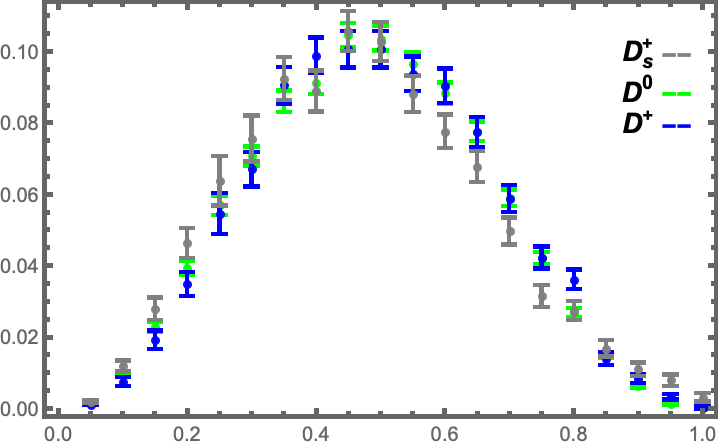
\includegraphics[width=0.8\textwidth]{figures/Dspectrum.png}
    \caption{实验室系下$\mrm{D}\to X e^+\nu_e$衰变过程归一化的电子能谱} % 添加图例
    \label{fig:cleo_D_sp}  % 添加标签
\end{figure}
    完整电子能谱数据点如图\ref{fig:cleo_D_sp}所示。

    $\mrm{D^{+}}$介子半轻单举衰变电子能谱的拟合外推与$\mrm{D^{0}}$介子基本一致,对应的电子能谱如图\ref{fig:cleo_D_sp}所示。
    上述讨论及结果将为我们抽取$\mrm{D^{0,+}}$介子的物理可观测量奠定基础。

本文的工作基于BESIII合作组的数据对$\mrm{D_s^+\to X e^+\nu_e}$过程物理可观测量进行抽取和全局拟合，与D介子处理方法类似，本文基于重夸克有效理论提出的拟合模型(式\eqref{func:fitting function})对表\ref{tab:BESIII_Ds_electron_sp}中前四个bin的数据进行拟合，随后基于拟合结果在积分意义上讲其标度转换至$\mrm{p_{e}< 0.2\GeV}$区域。

为实现更优的拟合效果，并使之与表\ref{tab:BESIII_Ds_electron_sp}中前四个bin的数据保持一致，需要在理论模型中引入标度因子，该因子包括$\mrm{D_s^+}$介子寿命、相应的量纲转换因子和一个经验系数s=1000。CKM矩阵元取值与上节一致。于$\mrm{D_s^+}$介子寿命的取值来源于PDG，为$(1033\pm 5)*10^{-15}s$。
\begin{equation}
    \Delta N_{i}=\frac{\Delta N_{i}}{N} N= \frac{\Delta \Gamma_{i}}{\Gamma}=\frac{1}{\Gamma} \frac{\mrm{d}\Gamma}{\mrm{d}E_{e}}d E_{e}=\frac{1}{\Gamma} \frac{\mrm{d}\Gamma}{\mrm{d}E_{e}}\Delta (E_e)_{i}=s g\tau_{D^{0}}\frac{\mrm{d}\Gamma}{\mrm{d}E_{e}}\Delta (E_e)_{i}, 
\end{equation}
总事例数N被吸收至$\frac{\mrm{d}\Gamma}{\mrm{d}E_{e}}$中并反映于拟合参数的拟合估计值上。

定义$\chi^{2}$函数如下，
\begin{equation}
    \chi^{2}=\sum_{i=1}^{4}(\frac{\Delta N_{i,\text{theory}}-\Delta N_{i,\text{exp}}}{\Delta N_{i,\sigma}})^2
\end{equation}
其中，$\Delta N_{i,\sigma}$是第i个bin的事例数的标准误差，$\Delta N_{i,\text{theory}}$是第i个bin事例数的理论预言，$\Delta N_{i,\text{exp}}$是第i个bin的事例数的实验观测中心值。
拟合结果为：
$$\chi^{2}_{min}=0.896179, a \rightarrow \hat{a}=188.748\pm 31.843, b \rightarrow \hat{b}=-0.641\pm 0.217$$

基于拟合结果，在积分意义上，将表\ref{tab:BESIII_Ds_electron_sp}前四个bin的数据延拓至$\mrm{p_e<0.2\GeV}$区域，可得对应区域的四个数据点。采用于D介子处理系统误差类似的方法可得$\mrm{D_s^+\to X e^+\nu_e}$过程的电子能谱。
同样的,我们做类似于$D^{0}$介子的非线性外推可得$\mrm{p}_{e}<0.2\GeV$区域的四个数据点。对应完整电子能谱如图\ref{fig:cleo_D_sp}所示。

基于拟合外推，可得三种D介子半轻单举衰变的完整电子能谱的数据集，后续将基于这些数据集进行物理可观测量的抽取。
\newpage
\subsection{物理可观测量的抽取}
本节将基于这三组数据集进行衰变分支比、衰变宽度、电子能量原点矩以及电子能量中心矩的抽取。此外本节还将给出这些物理可观测量之间的关联矩阵，并最终确定用于全局拟合的物理可观测量。
\subsubsection{一. 衰变宽度(衰变分支比)的抽取}
\paragraph{$\mrm{D^{0,+}}$介子} 对每个bin的第j个数据进行求和，即第j个衰变分支比； 第j个衰变宽度是$\mrm{\Gamma_{j}=\sum_{i=1}^{N_{bin}} x \Delta Br[i,j]/\tau}$，其中x是量纲转换因子，将$s^{-1}$转换到$\GeV$，$i=1,2,3,\cdots200000$.
\paragraph{$\mrm{D_{s}}$介子} 
由于探测器只能在超过某一动量阈值时才能识别和重建正电子轨迹，因此仅接受动量$\mrm{p}>0.2 \, \mathrm{GeV}$的双标记候选轨迹。作为电子动量$\mrm{p_e}$的函数，微分衰变分支比为：

\begin{equation}
    \mrm{\frac{d \mathcal{B}_{\mathrm{SL}}}{d p_\mrm{e}}=\frac{\Delta\left(\frac{n_{\mathrm{DT}}}{\epsilon_{\mathrm{DT}}}\right) / \Delta p_\mrm{e}}{n_{\mathrm{ST}} / \epsilon_{\mathrm{ST}}}=\frac{\left(\frac{\Delta n_{\mathrm{DT}}}{\epsilon_{\mathrm{Sig}}}\right) / \Delta p_\mrm{e}}{n_{\mathrm{ST}} \frac{e_{\mathrm{ST}}^{\prime}}{\epsilon_{\mathrm{ST}}}}=\frac{\Delta N_{\mathrm{DT}} / \Delta p_e}{n_{\mathrm{ST}} b_{\mathrm{tag}}}}.
\end{equation}

其中, $\mrm{n_{\mathrm{ST}}}$是观察到的单标记事件的事例数，$\mrm{\Delta n_{\mathrm{DT}}}$是在特定的$\mrm{p_e}$区间内观察到的半轻衰变双标记事件的事例数，$\mrm{\epsilon_{\mathrm{ST}}}$和$\mrm{\epsilon_{\mathrm{DT}}}$分别是单标记侧和双标记侧的重建效率。定义$\epsilon_{\mathrm{DT}}=\epsilon_{\mathrm{ST}}^{\prime} \times \epsilon_{\text{sig}}$，其中$\epsilon_{\text{sig}}$是信号侧具有电子动量依赖的重建效率，$\epsilon_{\mathrm{ST}}^{\prime}$是给定信号事件在反冲侧存在时的标记侧重建效率，$b_{\text{tag}} \equiv \frac{c_{\mathrm{ST}}}{\epsilon_{\mathrm{ST}}}$，它考虑了在反冲侧存半轻衰变时，单标记探测效率的差异，并且$\mrm{\Delta N_{\mathrm{DT}}}$是在特定$\mrm{p_e}$区间内的单标记样本中双标记信号事例的真实数量。对$\mrm{E}_{\mrm{e}}$进行积分可得衰变分支比的表达式:

\begin{equation}
    \mrm{\mathcal{B}\left(D_s^{+} \rightarrow X e^{+} \nu_e\right)=\frac{N_{\mathrm{DT}}}{n_{\mathrm{ST}} b_{\mathrm{tag}}}},
    \label{eq:BR_Ds}
    \end{equation}
    \begin{table}[h!]
        \scriptsize
        \centering
        \begin{tabular}{lc}
            \hline \hline Dataset & Fitted single-tag yields($n_{ST}$) \\
            \hline$E_{\mathrm{cm}}=4.178 \mathrm{GeV}$ & $147581 \pm 779$ \\
            $E_{\mathrm{cm}}=4.189-4.219 \mathrm{GeV}$ & $85845 \pm 705$ \\
            $E_{\mathrm{cm}}=4.225-4.230 \mathrm{GeV}$ & $29234 \pm 435$ \\
            Sum & $262660 \pm 1137$ \\
            \hline \hline
            \end{tabular}
        \caption{$\mrm{D_s^+\to X e^+\nu_e}$过程每个能量点的单标记产额}
        \label{tab:BESIII_Ds_singleyeilds_fit}
    \end{table}
其中，BESIII合作组基于MC模拟的$\mrm{b_{tag}}$和已经确定的单标记事例提供了每组数据中拟合得到的单标记产额\footnote{仅包含统计误差}(表\ref{tab:BESIII_Ds_singleyeilds_fit})和每组数据的$\mrm{\text{b}_{tag}}$（表\ref{tab:BESIII_Ds_btag}）
\begin{table}[htbp]
    \scriptsize
    \centering
    \begin{tabular}{lccc}
        \hline \hline Dataset & $\epsilon_{\text {ST }}$ & $b_{\text {tag }}$ & $b_{\text {tag }}^\tau$ \\
        \hline$E_{\mathrm{cm}}=4.178 \mathrm{GeV}$ & $(43.10 \pm 0.01) \%$ & $1.007 \pm 0.001$ & $1.037 \pm 0.003$ \\
        $E_{\mathrm{cm}}=4.189-4.219 \mathrm{GeV}$ & $(42.46 \pm 0.02) \%$ & $1.004 \pm 0.002$ & $1.034 \pm 0.004$ \\
        $E_{\mathrm{cm}}=4.225-4.230 \mathrm{GeV}$ & $(40.48 \pm 0.03) \%$ & $1.005 \pm 0.003$ & $1.044 \pm 0.007$ \\
        \hline \hline
        \end{tabular}
        \caption{$\mrm{D_s^+\to X e^+\nu_e}$过程每个能量点的单标记效率}
    \label{tab:BESIII_Ds_btag}
\end{table}
本文基于式\eqref{eq:BR_Ds},利用MC模拟计算$\mrm{D_s^{+} \rightarrow X e^{+} \nu_e}$过程的衰变分支比和的衰变宽度。
\begin{equation}
    \begin{aligned}
        \mathcal{B}\left(\mrm{D^0 \rightarrow X e^{+} \nu_e}\right)&=0.0636(15) ,\\
        \mathcal{B}\left(\mrm{D^{+} \rightarrow X e^{+} \nu_e}\right)&=0.1602(32),\\
        \mathcal{B}\left(\mrm{D_s^{+} \rightarrow X e^{+} \nu_e}\right)&=0.0631(14).\\
    \end{aligned}
    \label{eq:br_fit}
\end{equation}
基于上述讨论，$\mrm{D_s^+}$，$\mrm{D^0}$和$\mrm{D^+}$衰变分支比如上式所示，它们与BESIII，CLEO合作组的结果高度一致。
    
\subsubsection{二. 电子能量矩的抽取:以$\mrm{D_s}$介子为例}
理论上电子能量矩的定义如下，
\begin{equation}
    \langle \mrm{E_{e}^{n}}\rangle=\frac{1}{\Gamma}\int E_{e}^{n}\frac{d\Gamma}{d E_{e}} d E_{e},
    \label{eq:moment_theory}
\end{equation}
其中，$n=1,2,3,\cdots$。 实验测量过程中，为了方便起见将连续的电子能量相空间离散化并将积分转变为求和，
\begin{equation}
    \langle \mrm{E_{e}^{n}}\rangle=\frac{1}{\Gamma}\int \frac{d\Gamma}{d E_{\mrm{e}}} d E_{\mrm{e}}=(E_{\mrm{e}}^{n})_{i}\sum_{i}\frac{\Delta \Gamma_{i}}{\Gamma}=(E_{\mrm{e}}^{n})_{i}\sum_{i}\frac{\Delta \mrm{N}_{i}}{\mrm{N}},
    \label{eq:moment_exp}
\end{equation}
其中，N是总事例数，i是bin的编号。尽管实验测量过程中将相空间离散化成很多个bin且对每个bin内的数据不做区分，本文依然考虑了每个bin内电子能量的涨落，即认为第i个bin内的电子能量服从uniform distribution。
本文抽取出实验室系下的前四阶电子能量原点矩，如图\ref{fig:Moment_D0_lab}所示，
\begin{figure}[htbp]
    \centering
    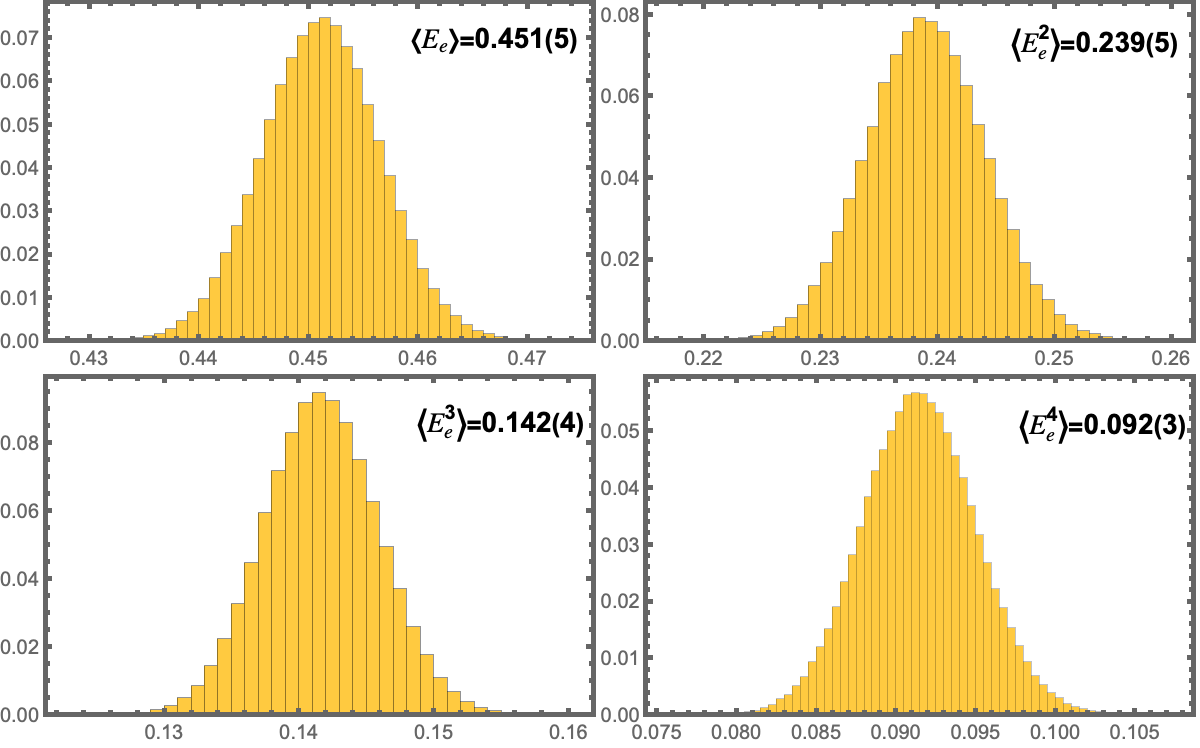
\includegraphics[width=1\textwidth]{figures/H1234.png}
    \caption{实验室系下$\mrm{D\to X e^+\nu_e}$衰变过程的前四阶电子能量矩的概率密度分布}
    \label{fig:Moment_D0_lab}  % 添加标签
\end{figure}

在与电子能量前四阶原点矩的理论表达式进行拟合之前，需通过洛伦兹变换将实验室系下的观测量转换至$\mrm{D_s^+}$质心系。电子能量在$\mrm{D_s^+}$在实验室系与质心系下的关系为：

\begin{equation}
E_{\mathrm{e}}^{\prime} = \gamma E_{\mathrm{e}}(1 - \beta \cos \theta),
\end{equation}
其中，$E_{\mathrm{e}}$ 是电子在 $\mrm{D_s^+}$质心系中的能量，$\beta, \gamma = 1/(\sqrt{1 - \beta^2})$ 是初级顶点上$\mrm{D_s^+}$ 介子的洛伦兹变换因子，$\theta$ 是电子动量在 $\mrm{D_s^+}$ 质心系中的方向与实验室参考系中 $\mrm{D_s^+}$ 介子动量之间的夹角。由于 $\mrm{D_s^+}$ 介子的自旋为零，$\theta$ 的分布是均匀的。可得实验室系下电子能量原点矩和质心系下电子能量原点矩之间的关系为：
\begin{equation}\label{eq:boost}
    \begin{aligned}
     \langle \mrm{E_e} \rangle_{\rm lab} &= \gamma \langle \rm E_e \rangle, & \quad \langle \rm E_e^2 \rangle_{\rm lab} &= \left( 1 + \frac{\beta^2}{3} \right) \gamma^2 \langle\rm E_e^2 \rangle, \\
     \langle \mrm{E_e^3} \rangle_{\rm lab} &= (1 + \beta^2) \gamma^3 \langle \rm E_e^3 \rangle, & \quad \langle \rm E_e^4 \rangle_{\rm lab} &= \left( 1 + 2 \beta^2 + \frac{\beta^4}{5} \right) \gamma^4 \langle \rm E_e^4 \rangle.
    \end{aligned}
  \end{equation}
表\ref{tab:BESIII_Ds_singleyeilds_fit}给出了BESIII合作组实际测量过程中使用的能量点和对应$D_{s}$的估计事例数。$\mrm{e^+ e^-}$对撞产生的$\mrm{D_{s},D^{*}_s}$在实验室系下的动量满足：
\begin{equation}
    \sqrt{p^2 + m_{\mrm{D_s}}^2} + \sqrt{p^2 + m_{\mrm{D_s^{*}}}^2} = E_{\mathrm{cm}},
\end{equation}
其中，$\mrm{D_s^+}$介子的质量为$1.96835\pm 0.00007\GeV$,$D^*_s$介子质量为$2.1122\pm0.0004\GeV$。本文在六个能量点上计算了对应$\mrm{D_s,D^*_s}$的洛伦兹因子$\gamma$,并将每个能量点上$\mrm{D_s^+}$介子的事例数作为权重进行加权求和。最终采用的$\gamma$是$\mrm{D_s^+}$和$\mrm{D_s^*}$介子的算术平均，
\begin{equation}
    \begin{aligned}
        \gamma&=1.02732 \pm 0.00009,\\
        \beta&= 0.2291 \pm 0.0004,\\
    \end{aligned}
    \end{equation}
由于洛伦兹变换因子不确定度较低，因此本文后续的分析将不考虑洛伦兹变换因子的误差。

    至此可得$\mrm{D_s}$静止系的电子能量前四阶矩。应用类似的方法，可得$\mrm{D^0}$,$\mrm{D^+}$介子质心系的电子能量前四阶矩为：
    \begin{equation}
        \scriptsize
        \begin{aligned}
        \left\langle E_e\right\rangle_{\rm exp}^{D_{s}}=0.439(5) \mathrm{GeV}, & \quad\left\langle E_e^2\right\rangle_{\rm exp}^{D_{s}}=0.223(5) \mathrm{GeV}^2, &\left\langle E_e^3\right\rangle_{\rm exp}^{D_{s}}=0.124(4) \mathrm{GeV}^3, &\quad \left\langle E_e^4\right\rangle_{\rm exp}^{D_{s}}=0.074(3) \mathrm{GeV}^4, \\
        \left\langle E_e\right\rangle_{\rm exp}^{D^0}=0.462(5) \mathrm{GeV}, &\quad\left\langle E_e^2\right\rangle_{\rm exp}^{D^0}=0.242(5) \mathrm{GeV}^2,  &\left\langle E_e^3\right\rangle_{\rm exp}^{D^0}=0.138(4) \mathrm{GeV}^3, & \quad\left\langle E_e^4\right\rangle_{\rm exp}^{D^0}=0.084(3) \mathrm{GeV}^4, \\
        \left\langle E_e\right\rangle_{\rm exp}^{D^{+}}=0.455(4) \mathrm{GeV}, & \quad\left\langle E_e^2\right\rangle_{\rm exp}^{D^{+}}=0.236(4) \mathrm{GeV}^2, &\left\langle E_e^3\right\rangle_{\rm exp}^{D^{+}}=0.134(3) \mathrm{GeV}^3, &\quad \left\langle E_e^4\right\rangle_{\rm exp}^{D^{+}}=0.081(3) \mathrm{GeV}^4. \\
        \end{aligned}
        \label{eq:momentRest}
        \end{equation}
    事实上，电子能量原点矩之间存在一定的关联，因此讨论其关联系数并尽可能的降低其关联程度是必要的。
    
    具体而言，本文通过计算皮尔逊积矩系数（Pearson's product-moment coefficient，PPMC）以实现电子能量矩的关联的定量分析。
    \begin{equation}
        \begin{aligned}
            \rho_{X, Y}&=\operatorname{corr}(X, Y)=\frac{\operatorname{cov}(X, Y)}{\sigma_X \sigma_Y}=\frac{\mathrm{E}\left[\left(X-\mu_X\right)\left(Y-\mu_Y\right)\right]}{\sigma_X \sigma_Y}, \quad \text { if } \sigma_X \sigma_Y>0 .\\
            &=\frac{\mathrm{E}(X Y)-\mathrm{E}(X) \mathrm{E}(Y)}{\sqrt{\mathrm{E}\left(X^2\right)-\mathrm{E}(X)^2} \cdot \sqrt{\mathrm{E}\left(Y^2\right)-\mathrm{E}(Y)^2}},
        \end{aligned}
        \end{equation}
        其中，X和Y是任意两组随机变量，\(\operatorname{E}\) 是期望值算符，\(\operatorname{cov}\) 是协方差，\(\operatorname{corr}\) 是PPMC的另一种符号，$\sigma$是随机变量的标准误差，事实上这是柯西-施瓦茨(Cauchy–Schwarz) 不等式的推论，要求即PPMC的绝对值不大于一。因此，相关系数的取值范围在 -1 和 +1 之间。当存在完全正向（递增）线性关系（相关）时，相关系数为 +1；当存在完全反向（递减）线性关系（反相关）时\ct{wearden1991statistics}，相关系数为 -1；在其他情况下，相关系数的值位于开区间 $(-1,1)$ 之间，表示变量之间的线性依赖程度。当相关系数接近零时，表示变量之间的关系较弱（接近无相关性）。相关系数越接近 -1 或 +1，变量之间的相关性越强。

        
    事实上PPMC仅表征两个变量之间的线性依赖程度，PPMC等于零是任意两组随机变量相互独立的必要条件，且无法完全表征两组随机变量之间的关系\ct{anscombe1973graphs}（PPMC是充分统计量的前提是随机变量服从多元正态分布）。
 
    本文讨论了三种D介子的衰变宽度和电子能量原点矩的关联矩阵，为确保准确性，通过散点分布图以实现视觉检查是必要的（$\mrm{D_s^+}$为例）。如图\ref{fig:Moment_Ds_joint}所示，自上（左）到下（右）分别是衰变宽度与电子能量前四阶原点矩。
        \begin{figure}[htbp]
            \centering
            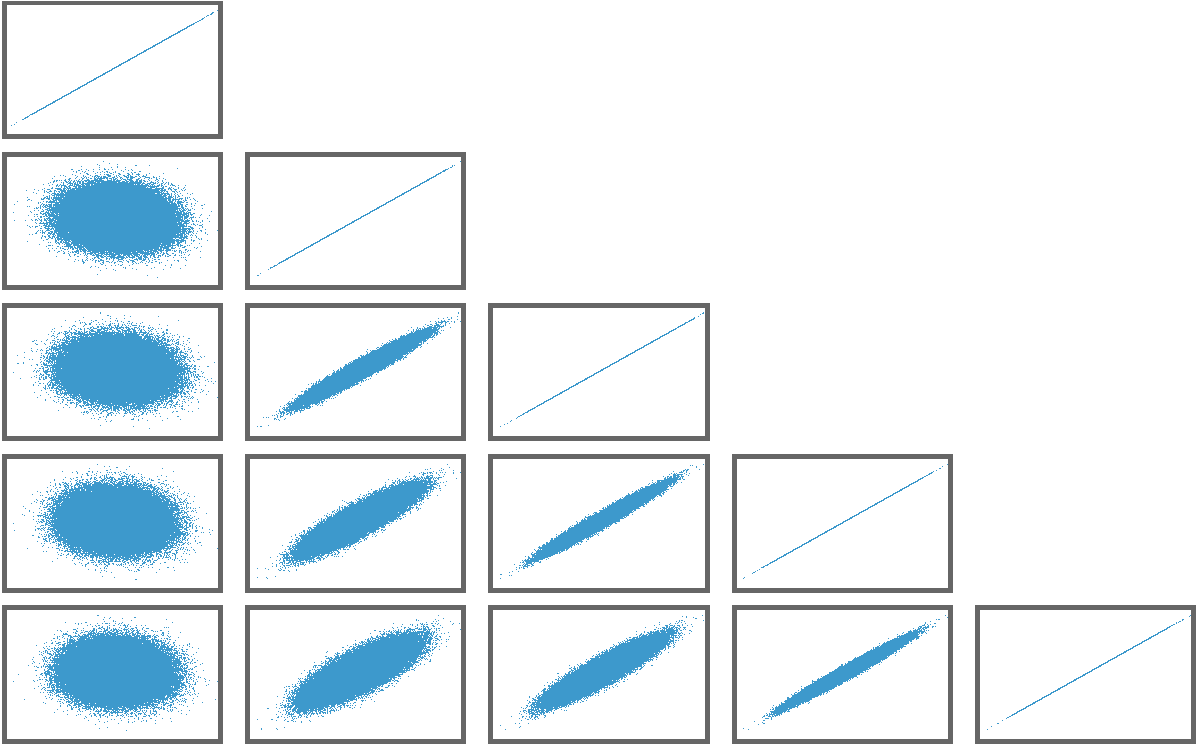
\includegraphics[width=1\textwidth]{figures/jonitsadian.png}
            \caption{$\mrm{D_s^+\to X e^+\nu_e}$衰变过程的衰变宽度与前四阶电子能量原点矩的联合分布}
            \label{fig:Moment_Ds_joint}  % 添加标签
        \end{figure}

        结果表明图\ref{fig:Moment_Ds_joint}与式\eqref{eq:cormoments}的结论保持一致，即衰变宽度与前四阶矩存在微弱负关联且电子能量i阶原点矩与电子能量j阶原点矩关联程度较强。
        \begin{align}\label{eq:cormoments}
            {\rm Cor}(D^0) &= \left(\begin{array}{ccccc}
            1 . & -0.0764818 & -0.0682164 & -0.0584038 & -0.049709 \\
            -0.0764818 & 1 . & 0.964628 & 0.888372 & 0.799743 \\
            -0.0682164 & 0.964628 & 1 . & 0.976053 & 0.921246 \\
            -0.0584038 & 0.888372 & 0.976053 & 1 . & 0.982859 \\
            -0.049709 & 0.799743 & 0.921246 & 0.982859 & 1 .
            \end{array}\right), \nonumber \\
            {\rm Cor}(D^+) &=\left(\begin{array}{ccccc}
            1 . & -0.00918393 & -0.0111696 & -0.011663 & -0.0114986 \\
            -0.00918393 & 1 . & 0.959852 & 0.877876 & 0.784972 \\
            -0.0111696 & 0.959852 & 1 . & 0.974619 & 0.917145 \\
            -0.011663 & 0.877876 & 0.974619 & 1 . & 0.982034 \\
            -0.0114986 & 0.784972 & 0.917145 & 0.982034 & 1 .
            \end{array}\right),\\
            {\rm Cor}(D^+_s) &=\left(\begin{array}{ccccc}
            1 . & -0.0948363 & -0.0854423 & -0.0692735 & -0.0528099 \\
            -0.0948363 & 1 . & 0.961103 & 0.877715 & 0.779303 \\
            -0.0854423 & 0.961103 & 1 . & 0.973193 & 0.910118 \\
            -0.0692735 & 0.877715 & 0.973193 & 1 . & 0.979699 \\
            -0.0528099 & 0.779303 & 0.910118 & 0.979699 & 1 .
            \end{array}\right). \nonumber 
            \end{align}
            
            为了实现对非微扰参数拟合估计的较强约束，降低物理可观测量之间的关联程度是必要的。本文发现存在一组物理可观测量，即$\mrm{D}$介子半轻单举衰变宽度，电子能量一阶原点矩，二三四阶中心矩，其关联程度显著降低。
               电子能量n阶中心矩的定义如下，
                \begin{align}
                    \left\langle \mrm{E_e^n}\right\rangle_{\rm center}\equiv \left\langle (E_e - \langle E_e\rangle)^n \right\rangle,
                    \end{align}
            此外本文也给出了该组物理可观测量的实验抽取结果（表\ref{tab:centermomentRest}）。为了避免该组物理可观测量之间的协方差矩阵出现病态行为\footnote{对某矩阵取逆，出现发散，则称原矩阵为病态矩阵。在计算机数值计算中，由于有限的精度，病态矩阵的逆可能会导致数值结果变得非常大或无穷大（即发散），使得结果没有意义}，需对该组物理可观测量进行重新标度。对应的重标度因子分别是，
            \begin{equation}
                \{10^{15}, 10^3, 10^3, 10^4,10^4\}
                \label{eq:rescaleonTOS}
            \end{equation}
            基于重标度因子可得该组物理可观测量重标度之后的关联矩阵（式\eqref{eq:corcenmoments}），
            \begin{table}[htbp]
                \centering
                \begin{tabular}{lccc}
                    \toprule
                     & \( \mrm{\left\langle E_e^2 \right\rangle_{\text{center}}}/\GeV^2\)  & \(\mrm{ \left\langle E_e^3 \right\rangle_{\text{center}}}/\GeV^3 \) & \(\mrm{ \left\langle E_e^4 \right\rangle_{\text{center}}}/\GeV^4 \)  \\
                    \midrule
                    \(\mrm{ D_s^+} \) & 0.0297(13) & 0.0004(4) & 0.0021(2) \\
                    \( \mrm{D^0} \) & 0.0287(12) & -0.0001(3) & 0.0019(1) \\
                    \(\mrm{D^+} \) & 0.0291(11) & -0.0002(3) & 0.0019(1) \\
                    \bottomrule
                \end{tabular}
                \caption{物理可观测量的实验观测值}
                \label{tab:centermomentRest}
            \end{table}
             \begin{align}\label{eq:corcenmoments}
                {\rm Cor}(D^0) &=\left(\begin{array}{ccccc}
                1 . & -0.0764818 & 0.0281587 & 0.0330765 & 0.0102788 \\
                -0.0764818 & 1 . & -0.088841 & -0.444378 & -0.0618813 \\
                0.0281587 & -0.088841 & 1 . & -0.00420729 & 0.817582 \\
                0.0330765 & -0.444378 & -0.00420729 & 1 . & -0.0351105 \\
                0.0102788 & -0.0618813 & 0.817582 & -0.0351105 & 1 .
                \end{array}\right), \nonumber\\
                {\rm Cor}(D^+) &=\left(\begin{array}{ccccc}
                1 . & -0.00918393 & -0.00799742 & 0.00816853 & -0.0107153 \\
                -0.00918393 & 1 . & -0.0423819 & -0.456701 & -0.0390424 \\
                -0.00799742 & -0.0423819 & 1 . & -0.0538756 & 0.809543 \\
                0.00816853 & -0.456701 & -0.0538756 & 1 . & -0.0924318 \\
                -0.0107153 & -0.0390424 & 0.809543 & -0.0924318 & 1 .
                \end{array}\right), \\
                {\rm Cor}(D^+_s) &=\left(\begin{array}{ccccc}
                1 . & -0.0948363 & 0.0254998 & 0.0800786 & 0.00809594 \\
                -0.0948363 & 1 . & -0.047314 & -0.40486 & -0.0191632 \\
                0.0254998 & -0.047314 & 1 . & 0.0763575 & 0.800281 \\
                0.0800786 & -0.40486 & 0.0763575 & 1 . & 0.172337 \\
                0.00809594 & -0.0191632 & 0.800281 & 0.172337 & 1 .
                \end{array}\right) . \nonumber
                \end{align}
                其中，每一行（列）自左（上）而（下）分别是D介子半轻单举衰变宽度，电子能量一阶矩，电子能量第二、三、阶中心矩。式\eqref{eq:corcenmoments}中的非对角元相比\ref{eq:cormoments}更接近零，这表明新的这组物理可观测量之间的关联强度比使用$\{$衰变宽度，电子能量前四阶原点矩$\}$显著降低。本文以$\mrm{D_s^+}$为对应的该组物理可观测量为例给出联合分布（图\ref{fig:Momentcenter_Ds_joint}）以实现视觉检验。
                \begin{figure}[hbtp]
                    \centering
                    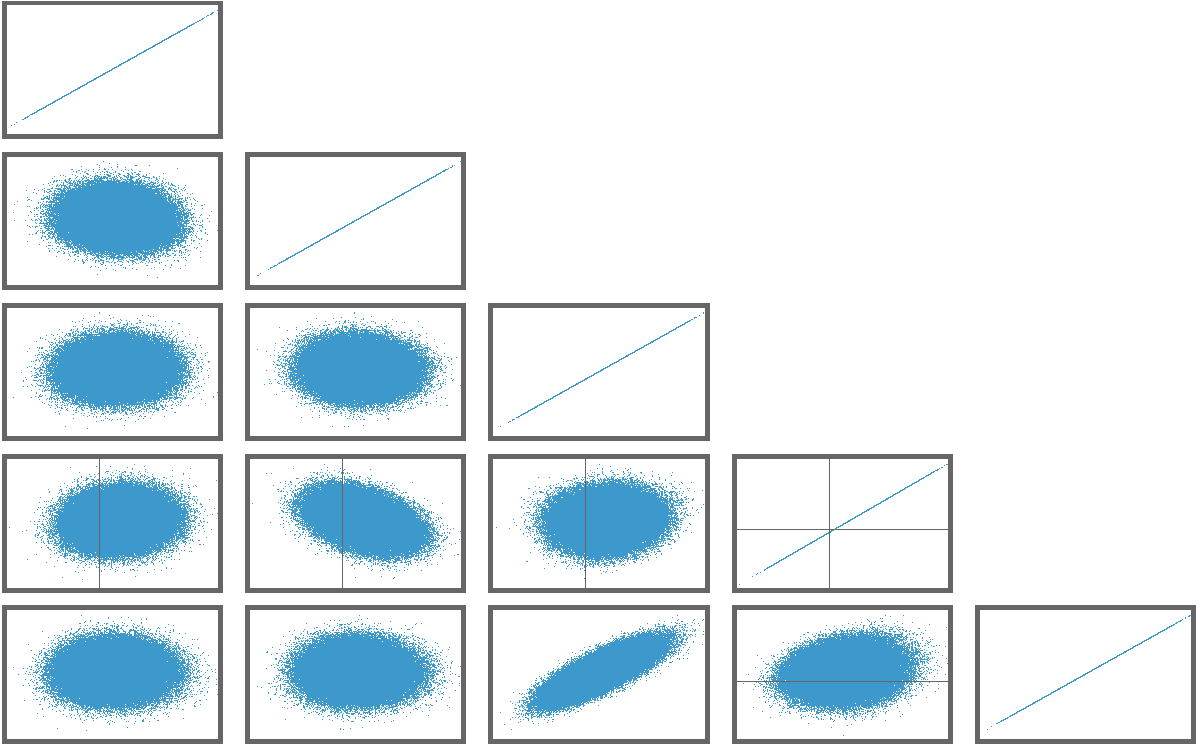
\includegraphics[width=1\textwidth]{figures/jonitsadiancenter.png}
                    \caption{$\mrm{D_s^+\to X e^+\nu_e}$衰变过程的衰变宽度、电子能量一阶原点矩与二、三、四阶中心矩的联合分布}
                    \label{fig:Momentcenter_Ds_joint}  % 添加标签
                \end{figure}

                本节以$\mrm{D_s^+}$为例讨论了电子能量原点矩的抽取，并将其转换到$\mrm{D_s^+}$的质心系;引入PPMC以讨论它们之间的关联强度(式\eqref{eq:cormoments})并与视觉检验（图\ref{fig:Moment_Ds_joint}）形成交叉检验。结果表明：电子能量前四阶原点矩之间存在较强关联，为了对非微扰参数实现更强约束，本文重新抽取了一组物理可观测量：衰变宽度、电子能量一阶原点矩和电子能量第二、三、四阶中心矩。同样地，本文也讨论了它们的关联程度（式\eqref{eq:corcenmoments}和图\ref{fig:Momentcenter_Ds_joint}）。结果表明新的一组物理可观测量之间的关联强度普遍比前者要显著降低，这将有助于对非微扰参数的拟合估计提供更强约束。
                %%%%%%%%%%%%%%%%%%%%%%%%%%%%%%%
\subsection{重夸克质量方案}

第三章在Pole mass scheme下给出了衰变宽度和电子能量前四阶原点矩的理论表达式，并且发现物理可观测量对粲夸克质量高度敏感。事实上用作为重夸克有效理论拉格朗日量参数之一的Pole mass表示的衰变宽度，其高阶微扰修正收敛性非常差。此外不同的charm mass scheme下的粲夸克质量不确定度较低，由于物理可观测量有限，因此本文不对粲夸克质量进行抽取。

由于量子色动力学的夸克禁闭效应导致实验上无法直接测量夸克质量，因此选择适当的质量方案对D介子衰变宽度的理论计算具有关键性的作用。

在壳重整化方案要求在微扰论的每一阶重夸克传播子的逆等于零，对应的重夸克质量称为极质量。尽管极质量作为重夸克有效理论的基本参数之一，但这种质量定义并不是一个好的选择，因为它存在重整化模糊性。这种模糊性表现为极点质量与短程质量的微扰展开级数的收敛性较差，例如在重整化能标$\mu=1.27\GeV$处极质量和$\overline{\mrm{MS}}$质量之间的转换关系为：
\begin{equation}
    \begin{aligned}
    m_\mrm{c}^{\text {Pole }} & =\bar{m}_\mrm{c}\left(\bar{m}_\mrm{c}\right)\left[1+\frac{4}{3} \frac{\alpha_s\left(\bar{m}_c\right)}{\pi}+10.43\left(\frac{\alpha_s\left(\bar{m}_c\right)}{\pi}\right)^2+116.5\left(\frac{\alpha_s\left(\bar{m}_c\right)}{\pi}\right)^3+\cdots\right] \\
    & =\bar{m}_\mrm{c}\left(\bar{m}_\mrm{c}\right)[1+0.1642+0.1582+0.2176+\cdots].
    \end{aligned}
    \end{equation}
    事实上，如果使用$\overline{\mrm{MS}}$质量表示D介子单举衰变宽度，由于重整化能标过于靠近非微扰区域导致其微扰级数的收敛性同样不理想，另一方面，在非常低的尺度下， 
    $\overline{\mrm{MS}}$质量的对数演化是非物理的\ct{Melnikov:2000qh}。为了获得收敛行为良好的微扰展开级数需要合适的粲夸克质量方案。在底强子单举衰变中应用非常成功的质量方案被称为动力学质量方案，其截断能标远离非微扰区域。动力学质量方案和极质量方案之间的关系为\ct{Bigi:1994ga}：
      \begin{equation}
        m_\mrm{Q}^{\text {kin }}(\mu)=m_\mrm{Q}^{\text {Pole }}-[\bar{\Lambda}(\mu)]_{\text {pert }}-\frac{1}{2 m_\mrm{Q}^{\text {kin }}(\mu)}\left[\mu_\pi^2(\mu)\right]_{\text {pert }}+\mathcal{O}\left(\frac{1}{\left(m_\mrm{Q}^{\text {kin }}\right)^2}\right),
        \end{equation}
    其中Q是重夸克,$\bar{\Lambda}$ 和 $\mu_\pi^2$的领头阶的表达式为\ct{Bigi:1994ga}：
        \begin{equation}
            \begin{aligned}
            & {[\bar{\Lambda}(\mu)]_{\mathrm{pert}}=\frac{16}{9} \frac{\alpha_s}{\pi} \mu+\mathcal{O}\left(\alpha_s^2\right)}, \\
            & {\left[\mu_\pi^2(\mu)\right]_{\mathrm{pert}}=\frac{4}{3} \frac{\alpha_s}{\pi} \mu^2+\mathcal{O}\left(\alpha_s^2\right)},
            \end{aligned}
            \end{equation}
    $\mu$是截断能标。在动力学质量方案下，极质量中的微扰级数被$[\bar{\Lambda}(\mu)]_{\text {pert }}$ 和 $\left[\mu_\pi^2(\mu)\right]_{\text {pert }}$修改。此外，重夸克有效理论中的参数也将被重新定义\ct{Gambino:2007rp, Gambino:2017vkx}，
    \begin{equation}
        \begin{aligned}
        \mu_\pi^2 & =\mu_\pi^{2, \mathrm{kin}}+\left[\mu_\pi^2(\mu)\right]_{\mathrm{pert}}=\mu_\pi^{2, \mathrm{kin}}+\frac{4}{3} \frac{\alpha_s}{\pi} \mu^2, \\
        \rho_D^3 & =\rho_D^{3, \mathrm{kin}}+\left[\rho_D^3(\mu)\right]_{\mathrm{pert}}=\rho_D^{3, \mathrm{kin}}+\frac{8}{9} \frac{\alpha_s}{\pi} \mu^3.
        \end{aligned}
        \end{equation}
        重夸克有效理论中$\mrm{(\Lambda_{QCD}/m_{Q})^{n}}$的项产生了 $\mrm{\left(\frac{\alpha_s}{\pi}\right) \frac{\mu^n}{m_Q^n}}$ 阶的修正，这使得截断尺度的选择窗口很小。一方面，它必须比重夸克质量小，使得 $\frac{\mu}{m_\mrm{Q}}$ 是一个收敛行为良好的展开参数；另一方面，它应该处于微扰区域。截断能标在$\mu= 1\GeV$的动力学质量方案已成功应用于B介子单举衰变（参见例如\ct{Alberti:2014yda,Gambino:2016jkc}）。

        对于本文研究的粲介子单举衰变若存在类似的动力学质量方案，则其截断能标$\mu$的选择窗口显著降低。

        本文采用的质量方案之一是$\overline{\mrm{MS}}$质量方案，并在两圈图水平上将其转换为极质量\ct{Chetyrkin:2000yt}，如式\eqref{eq:MSbar}所示，
        \begin{equation}
            \begin{aligned}
                m_{\text{c}}^{\text{pole}} = m_{\text{c}} &+ m_{\text{c}}\frac{\left(\frac{4}{3} + \log \left[\frac{\mu^2}{m_{\text{c}}^2}\right]\right) \alpha_s}{\pi} \\
                &+m_{\text{c}} \frac{\alpha_s^2\left(\frac{779}{96} + \frac{\pi^2}{6} + \frac{1}{9} \pi^2 \log [2] + \frac{415}{72} \log \left[\frac{\mu^2}{m_{\text{c}}^2}\right] + \frac{37}{24} \log \left[\frac{\mu^2}{m_{\text{c}}^2}\right]^2 - \frac{\zeta(3)}{6}\right)}{\pi^2},
            \end{aligned}
                \label{eq:MSbar}
            \end{equation}

        其中，$m_{\mrm{c}}$是$\mrm{\overline{MS}}$质量方案下的粲夸克质量，$m_{\mrm{c}}^{\text{pole}}$是极质量方案下的粲夸克质量，$\mu$是重整化能标。
        
        本文采用的另外一个质量方案是1S质量方案，1S质量主要应用于夸克的束缚态质量，如底夸克和粲夸克，尤其是在强相互作用下产生的夸克对中，比如$\Upsilon$和$J/\psi$这样的$q\bar{q}$束缚态。文献\ct{Hoang:1998ng}给出了两圈图水平上1S质量和极质量之间的转换关系。对其取逆并展开到$\epsilon^2$阶，得到极质量与1S质量之间的转换关系，如式\eqref{eq:1S}所示,
        \begin{equation}
            m_\mrm{c}^{\text{Pole}}=m_\mrm{c}+\frac{2}{9} m_\mrm{c}\epsilon \alpha_s^2-\frac{\epsilon^2 m_\mrm{c}\left(-\frac{12992 \alpha_s^3}{9}-\frac{3200}{3} \log \left[\frac{3 \mu}{4 m_\mrm{c} \alpha_s}\right] \alpha_s^3-\frac{256 \pi \alpha_s^4}{9}\right)}{576\pi},
            \label{eq:1S}
        \end{equation}
        其中，$m\mrm{c}$是1S质量方案下的粲夸克质量，$\epsilon$是1S质量方案下的展开参数，$\epsilon$的线性项表示单圈水平，平方项表示两圈图水平。取$J/\psi$质量的1/2作为粲夸克的1S质量，即$m_{\mrm{c}}=1.55\GeV$。
        此外本文计算了1S质量方案下$\mrm{D}$介子半轻单举衰变宽度的微扰展开级数为
        \begin{equation}
            \Gamma_{\mrm{sl}}^{\mrm{D}}\sim 1-0.131-0.048+0.019+\cdots,
        \end{equation}
        从左至右分别是领头阶(Leading Order, LO)，次领头阶(Next to leading Order, NLO)，次次领头阶(Next Next to leading Order, NNLO)和次次次领头阶（Next Next Next to leading Order, NNNLO）的修正($\mrm{\alpha_s=0.387}$)。极质量方案下D介子半轻单举衰变宽度的微扰展开级数为
        $$\Gamma_{\mrm{sl}}^{\mrm{D}}\sim1-0.768104 \alpha_s-2.37521 \alpha_s^2-10.7295 \alpha_s^3+\cdots,$$
        收敛行为较差。因此，1S质量方案是比较合适的粲夸克质量方案，本文的唯象学分析将讨论$\overline{\text{MS}}$和1S质量方案下的全局拟合。
\subsection{唯象学分析}
为从$\mrm{D}$介子半轻单举衰变的实验数据中实现重夸克有效理论非微扰参数的拟合估计。本文采用$\mrm{D\to X_{\rm{c},\rm{s}} e^+ \nu_{e}}$过程的衰变宽度，电子能量一阶原点矩与电子能量第二、三、四阶中心矩的实验观测值和相应理论表达式进行全局拟合。在幂次修正精确至量纲六算符的精度下，包含以下的微扰参数：
\begin{equation}
    \begin{aligned}
        &\mu_{\pi}^2(\mrm{D^{0,+}}),\quad \mu_{\mrm{G}}^{2}(\mrm{D^{0,+}}),\quad \rho_{\mrm{D}}^3(\mrm{D^{0,+}}),\quad \rho_{\mrm{LS}}^3(\mrm{D^{0,+}}), \\
        &\mu_{\pi}^2(\mrm{D_s^+}),\quad\;\:\; \mu_{\mrm{G}}^{2}(D_s^+),\quad\;\:\: \rho_{\mrm{D}}^3(D_s^+),\quad\;\:\; \rho_{\mrm{LS}}^3(\mrm{D_s^+}),
    \end{aligned}
    \end{equation}
    
    
    
    

其中，由于同位旋对称性的约束，对$\mrm{D^{0}}$和$\mrm{D^{+}}$的非微扰参数不作区分。这些非微扰参数在粲介子寿命的理论计算，粲介子稀有衰变，甚至底介子的单举衰变中扮演了举重若轻的角色。量纲六算符也包含四夸克算符，基于真空插入近似\ct{Bauer:1986bm}（Vacuum Insertion Approximation， VIA）,四夸克算符非微扰矩阵元矩阵元对衰变宽度的贡献可以忽略不计。

为了讨论幂次展开的收敛性对拟合抽取重夸克有效理论中非微扰参数的影响，我们将在两种情形下进行全局拟合。对于情形$\mrm{I}$，物理可观测量的理论表达式的幂次修正仅精确至量纲五算符的贡献；对于情形$\mrm{II}$, 物理可观测量的理论表达式的幂次修正仅精确至量纲六算符的贡献。此外基于上节的讨论，本节将讨论三种不同的质量方案下非微扰参数的拟合估计。

由于重整化能标$\mu$的跑动会引起强相互作用耦合常数的浮动，因此讨论理论输入参数的误差对拟合估计非微扰参数的影响是必要的，经过对所有理论输入参数的误差评估，最终仅引入由于重整化能标的跑动导致强相互作用耦合常数的浮动误差。具体地，首先固定相关的理论输入参数并进行相关的全局拟合估计，对应非微扰参数的估计值作为非微扰参数的拟合估计中心值，对应非微扰参数的估计误差作为非微扰参数误差的实验部分；其次，使用MC技术完成2000次的相关拟合，取相关拟合关于非微扰参数的估计值分布的标准误差作为非微扰参数误差的理论部分。本文粗略地假设非微扰参数误差的理论部分和实验部分相互独立，基于误差传递公式得到非微扰参数的拟合估计误差。

在拟合过程中，本文使用了奇异夸克质量的 $2+1+1$ 格点 QCD FLAG 平均值，$\overline{m}_s(2 \mathrm{GeV}) = 93.44$ MeV~\cite{FlavourLatticeAveragingGroup:2019iem}。对于粲夸克质量，本文使用 $m_{c}^{\overline{\mrm{MS}}} = 1.27$ GeV 和 $m_{c,\mathrm{1S}} = 1.55$ GeV~\cite{ParticleDataGroup:2024cfk}。对于强耦合常数，本文采用Lenz等人在~\cite{King:2021xqp} 中通过 RunDec 包~\cite{Herren:2017osy} 获得的强相互作用耦合常数 $\alpha_{s}(\ov{m}_{c}) = 0.387$。对于 $\alpha_s(\mu)$ 和 $\ov{m}_c(\mu)$，本文考虑了从 1 GeV 到 $2\ov{m}_{c}(\ov{m}_{c})$ 的跑动 $\mu$。此外使用以下输入值用于理论公式中的其他参数~\cite{ParticleDataGroup:2024cfk}，$\mrm{G_F} = 1.1663788 \times 10^{-5}$，$\mrm{|V_{cs}|} = 0.975$，以及 $\mrm{|V_{cd}|} = 0.221$.

\subsubsection{一. 固定理论输入参数}
基于本文第三章理论部分的研究，可得到了三种D介子在极质量方案下的的衰变宽度，电子能量一阶原点矩与电子能量第二、三、四阶中心矩的理论表达式。此外本文提供了$\overline{\mrm{MS}}$ 和$\mrm{1S}$质量方案下物理可观测量微扰修正部分的理论表达式（附录\ref{app:TOS}）

定义物理可观测量的理论表达式\footnote{在实际全局拟合过程中，需要对$\aleph$的每个元素乘以式\eqref{eq:rescaleonTOS}相对应的标度因子}是集合$\aleph$，
\begin{equation}
    \begin{aligned}
        \aleph_{theory}^{D^{0}} := & \{\Gamma^{D^{0,+}}, \langle E_{e}\rangle^{D^{0,+}}, \langle E_{e}^2\rangle^{D^{0,+}}_{\text{center}}, \langle E_{e}^3\rangle^{D^{0,+}}_{\text{center}}, \langle E_{e}^4\rangle^{D^{0,+}}_{\text{center}}\}, \\
        \aleph_{theory}^{D^{+}} := & \{\Gamma^{D^{0,+}}, \langle E_{e}\rangle^{D^{0,+}}, \langle E_{e}^2\rangle^{D^{0,+}}_{\text{center}}, \langle E_{e}^3\rangle^{D^{0,+}}_{\text{center}}, \langle E_{e}^4\rangle^{D^{0,+}}_{\text{center}}\}, \\
        \aleph_{theory}^{D_s} := & \{\Gamma^{D_{s}},\langle E_{e}\rangle^{D_{s}}, \langle E_{e}^2\rangle^{D_{s}}_{\text{center}}, \langle E_{e}^3\rangle^{D_{s}}_{\text{center}}, \langle E_{e}^4\rangle^{D_{s}}_{\text{center}}\}.
    \end{aligned}
    \label{eq:TOS}
\end{equation}
重标度后对应的物理可观测量的实验观测值为：
\begin{equation}
    \begin{aligned}
        \aleph_{\text{exp, rescaled}}^{D^0} &:= \{102.137,461.653,28.7391,-1.10121,19.1876\}, \\
        \aleph_{\text{exp, rescaled}}^{D^+} &:=\{102.192,455.073,29.0727,-2.36531,19.7269\},\\
        \aleph_{\text{exp, rescaled}}^{D_s} &:=\{82.9754,439.393,29.6515,3.43014,21.3503\},\\
        \sigma(\aleph_{\text{exp, rescaled}}^{D^0})&:=\{2.40402,4.92835,1.21868,3.36424,1.33466\},\\
        \sigma(\aleph_{\text{exp, rescaled}}^{D^+})&:=\{2.03942,4.23467,1.1135,3.1932,1.22891\},\\
        \sigma(\aleph_{\text{exp, rescaled}}^{D_s})&:=\{1.98213,5.18726,1.29376,3.90018,1.6387\},\\
    \end{aligned}
    \label{eq:expdata}
\end{equation}
前三行是这组物理可观测量$\aleph$的中心值，后三行是这组物理可观测量$\aleph$的标准误差。

一般地，在 $n$ 个观测点通过测量得到一组 $n$ 个观测值 $\boldsymbol{y}=$ $\left(y_1, y_2, \cdots, y_n\right)^{\mathrm{T}}$ ，相应的观测值真值 $\boldsymbol{\eta}=\left(\eta_1, \eta_2, \cdots, \eta_n\right)^{\mathrm{T}}$ 为末知，它由某个理论
模型预期：$\eta_i=f\left(x_i, \boldsymbol{\theta}\right)(i=1,2, \cdots, n)$ ，其中 $\boldsymbol{\theta}=\left(\theta_1, \theta_2, \cdots, \theta_k\right)^{\mathrm{T}}$ 是待定的参数． $\theta$ 的最小二乘估计可由最小二乘函数 $Q^2(\boldsymbol{\theta})$ 的极小值求得
\begin{equation}
    Q^2(\boldsymbol{\theta})=(\boldsymbol{y}-\boldsymbol{\eta}(\boldsymbol{\theta}))^{\mathrm{T}} \boldsymbol{V}^{-1}(\boldsymbol{y}-\boldsymbol{\eta}(\boldsymbol{\theta}))=\sum_{i=1}^n \sum_{j=1}^n\left(y_i-\eta_i\right) V_{i j}^{-1}\left(y_j-\eta_j\right),
    \end{equation}
其中，$\boldsymbol{\theta}$是某个理论所包含的参数，$V$是测量值之间的协方差矩阵，若这组观测量之间相互独立，则$ Q^2(\boldsymbol{\theta})$约化为：$$
Q^2(\boldsymbol{\theta})=\sum_{i=1}^n\left(\frac{y_i-\eta_i}{\sigma_i}\right)^2,
$$
其中，$\sigma_{i}$是第i个测量值的标准误差。
定义最小二乘函数构造如下\footnote{l=u,d,s分别对应于$\mrm{D^{0}}, \mrm{D^{+}},\mrm{D_s^+}$}，
\begin{equation}
    \begin{aligned}
        Q^2(\boldsymbol{\theta})=&\sum_{l=u,d,s}\sum_{i=1}^{5}\sum_{j=1}^{5}\times\\
        &(\aleph_{\text{exp, rescaled}, i}^{D^l}-\aleph_{\text{theory, rescaled, i}}^{D^l})V_{i j,l}^{-1}(\aleph_{\text{exp, rescaled} ,j}^{D^l}-\aleph_{\text{theory, rescaled, j}}^{D^l})^{\text{T}},\\
    \end{aligned}
    \label{eq:chi2_func}
\end{equation}
其中$V_{ij,l}$是$\mrm{D^{l}}$介子五组数据之间的协方差矩阵。基于Mathematica进行非微扰参数的全局拟合估计，采用 DifferentialEvolution, SimulatedAnnealing, RandomSearchd等算法对搜索到的全局最小点进行交叉检验。此外本文基于Python完成了固定理论输入参数的前提下两种情形的全局拟合估计作为进一步交叉检验。
\paragraph{极质量方案}
我们选取两圈图水平上的极质量，即$m_{\mrm{c}}=1.67\GeV$.
拟合结果表明，对于情形$\mrm{I}$, $\chi^{2}_{\text{min}}=195.522$, $\chi^{2}_{\text{min}}/\text{d.o.f}=17.77$
\begin{equation}
    \mu_{\pi}^2(\mrm{D^{0,+}})\to 0.05,\;\mu_{\mrm{G}}^{2}(\mrm{D^{0,+}})\to -0.02, \;\mu_{\pi}^2(\mrm{D_s^+})\to 0.06, \;\mu_{\mrm{G}}^{2}(\mrm{D_s^+})\to 0.08
\end{equation}
对于情形$\mrm{II}$, $\chi^{2}_{\text{min}}=26.24$, $\chi^{2}_{\text{min}}/\text{d.o.f}=3.74$
\begin{equation}
    \begin{aligned}
        &\mu_{\pi}^2(\mrm{D^{0,+}})\to 0.11,\;\mu_{\mrm{G}}^{2}(\mrm{D^{0,+}})\to -0.03, \;\mu_{\pi}^2(\mrm{D_s^+})\to 0.15, \;\mu_{\mrm{G}}^{2}(\mrm{D_s^+})\to 0.08\\
        &\rho_{\mrm{D}}^3(\mrm{D^{0,+}})\to -0.005,\;\rho_{\mrm{LS}}^3(\mrm{D^{0,+}})\to 0.006, \;\rho_{\mrm{D}}^3(\mrm{D_s^+})\to -0.007, \;\rho_{\mrm{LS}}^3(\mrm{D_s^+})\to 0.007
    \end{aligned}
\end{equation}
极质量方案下D介子半轻单举衰变宽度的高阶微扰修正和幂次修正的收敛性较差，下面仅讨论$\overline{\mrm{MS}}$质量方案和$\mrm{1S}$质量方案下的拟合估计结果和相应误差分析。
\paragraph{$\overline{\mrm{MS}}$质量方案}
上一节我们讨论了两圈图水平上$\overline{\mrm{MS}}$质量和极质量之间的转换关系（式\eqref{eq:MSbar}）。将$\aleph_{\text{theory}}$中的物理可观测量在两圈图水平上用$\overline{\mrm{MS}}$质量表示出来(其微扰部分的具体形式见附录\ref{app:TOS}), 重整化能标取在粲夸克$\overline{\mrm{MS}}$质量处，即$\mu=1.27\GeV$,全局拟合估计结果如表\ref{tab:MS_fitting}所示
\begin{table}[h!]
    \scriptsize
    \begin{tabular}{cllllll} % 使用 | 添加竖线
    \hline
      $\mathrm{\overline{MS}}$ 方案&$\chi^2_{\text{tot}}$&$\mrm{D_{i}}$&$\mrm{\mu_{\pi}^{2}}$/$\mathrm{GeV^2}$&$\mrm{\mu_{G}^{2}}$/$\mathrm{GeV^2}$&$\mathrm{\rho_{D}^{3}}$/$\mathrm{GeV^3}$ &$\mrm{\rho_{LS}^{3}}$/$\mathrm{GeV^3}$ \\ % 表格内容
      \hline
     \multirow{2}{*}{\text{情形I}} & \multirow{2}{*}{\scriptsize{49.26}}  & $\mrm{D^{0,+}}$&\scriptsize{$0.09\pm0.01\pm.$}&\scriptsize{$0.27\pm 0.01\pm0.14$}&-&-\\
     &&$\mrm{D_s^+}$&\scriptsize{$0.09\pm 0.01\pm$0.01}&\scriptsize{$0.39\pm 0.01\pm 0.12$}&-&-\\
      \hline
      \multirow{2}{*}{\text{情形II}}  &  \multirow{2}{*}{\scriptsize{14.53}}  & $\mrm{D^{0,+}}$ &\scriptsize{$0.11\pm0.01\pm0.02$}&\scriptsize{$0.26\pm 0.01\pm0.14$}&\scriptsize{$-0.002\pm 0.001\pm0.001$}&\scriptsize{$0.003\pm 0.001\pm0.001$}\\
      &&$\mrm{D_s^+}$&\scriptsize{$0.12\pm0.01\pm0.02$}&\scriptsize{$0.38\pm0.01\pm0.13$}&\scriptsize{$-0.003\pm0.001\pm 0.001$}&\scriptsize{$0.005\pm 0.001\pm0.001$}\\  \hline
    \end{tabular}
    \caption{$\overline{\mrm{MS}}$质量方案下对非微扰参数的全局拟合估计结果}
    \label{tab:MS_fitting}
    \end{table}
    表\ref{tab:MS_fitting}中的第一个误差来源于实验，第二个误差来源于强相互作用耦合常数跑动带来的理论误差。情形$\mrm{I}$和$\mrm{II}$关于非微扰参数的拟合估计值非常接近，这反映了幂次修正的收敛行为较好。
\paragraph{$\mrm{1S}$质量方案}两圈图水平上1S质量和极质量之间的转换关系及其对重整化能标的具体依赖形式（式\eqref{eq:1S}），将$\aleph_{\text{theory}}$中的物理可观测量在两圈图水平上用$\mrm{1S}$质量表示出来(其微扰部分的具体形式见附录\ref{app:TOS}), 重整化能标取在粲夸克$\overline{\mrm{MS}}$质量处，即$\mu=1.27\GeV$,全局拟合结果如表\ref{tab_1S_fitting}所示,
\begin{table}[h!]
    \scriptsize
    \begin{tabular}{cllllll} % 使用 | 添加竖线
    \hline
     1S 质量方案&$\chi^2_{\text{tot}}$&$\mrm{D_{i}}$&$\mu_{\pi}^{2}$/$\mathrm{GeV^2}$&$\mu_{\mrm{G}}^{2}$/$\mathrm{GeV^2}$&$\mathrm{\rho_{\mrm{D}}^{3}}$/$\mathrm{GeV^3}$ &$\rho_{\mrm{LS}}^{3}$/$\mathrm{GeV^3}$ \\ % 表格内容
      \hline
     \multirow{2}{*}{\text{情形} I} & \multirow{2}{*}{\scriptsize{54.06}}  & $\mrm{D^{0,+}}$&\scriptsize{$0.04\pm0.003\pm0.010$}&\scriptsize{$0.33\pm 0.01\pm0.01$}&-&-\\
     &&$\mrm{D_s^+}$&\scriptsize{$0.06\pm 0.01\pm 0.01$}&\scriptsize{$0.44\pm 0.01\pm 0.02$}&-&-\\
      \hline
      \multirow{2}{*}{\text{情形} II}  &  \multirow{2}{*}{\scriptsize{$2.32$}}  & $\mrm{D^{0,+}}$&\scriptsize{$0.09\pm0.01\pm 0.01$}&\scriptsize{$0.32\pm0.01\pm0.01$}&\scriptsize{$-0.003\pm0.001\pm0.001$}&\scriptsize{$0.004\pm 0.001\pm0.001$} \\
      &&$\mrm{D_s^+}$&\scriptsize{$0.11\pm0.01\pm0.01$}&\scriptsize{$0.43\pm 0.01\pm0.02$}&\scriptsize{$-0.004\pm 0.001\pm0.001$}&\scriptsize{$0.005\pm0.001\pm0.001$}\\  \hline
    \end{tabular}
    \caption{1S质量方案下对非微扰参数的全局拟合结果}
    \label{tab_1S_fitting}
    \end{table}
    表\ref{tab_1S_fitting}中的第一个误差来源于实验，第二个误差来源于强相互作用作用耦合常数跑动引入的误差。1S 质量方案情形$\mrm{II}$的平均最小卡方值小于一，即在这种情形下具有良好的拟合效果；此外1S质量方案下幂次修正对非微扰参数的估计值影响同样较弱。


    %%%%%%%%%%%%%%%%%%%%%%%%%%%%%%%%%%%%%%
    此外本文计算了1S质量方案下情形$\mrm{II}$中非微扰参数拟合估计的关联矩阵（式\eqref{eq:corpara}），
    \begin{align}\label{eq:corpara}
        {\rm Cor}(D^{0,+})&=
        \left(\begin{array}{cccc}
        1 . & -0.247711 & -0.920525 & 0.85145 \\
        -0.247711 & 1 . & 0.325483 & -0.325445 \\
        -0.920525 & 0.325483 & 1 . & -0.971566 \\
        0.85145 & -0.325445 & -0.971566 & 1 .
        \end{array}\right), \\
        {\rm Cor}(D_{s}^+)&=
        \left(\begin{array}{cccc}
        1 . & -0.256407 & -0.901138 & 0.842813 \\
        -0.256407 & 1 . & 0.324073 & -0.32296 \\
        -0.901138 & 0.324073 & 1 . & -0.97023 \\
        0.842813 & -0.32296 & -0.97023 & 1 .
        \end{array}\right), \nonumber
        \end{align}
        式\eqref{eq:corpara}自上（左）而（右），分别是$\mu_{\pi}^{2}$, $\mu_{\mrm{G}}^{2}$, $\rho_{\mrm{D}}^{3}$,和$\rho_{\mrm{LS}}^3$。
    情形$\mrm{II}$相比于情形$\mrm{I}$而言，由于引入了量纲六算符的微扰参数使得最小卡方值迅速降低，表明量纲六算符的非微扰矩阵元的贡献在物理可观测量计算中具有举足轻重的作用，且此现象的存在与否并不依赖于粲夸克质量方案。这一事实确信了量纲六算符修正对物理可观测量的理论预言非常重要。由于物理可观测量有限，暂时无法实现对量纲六算符中四夸克算符的非微扰矩阵元的拟合估计。期待未来构建足够多的物理可观测量得以进行更丰富的全局拟合估计，从而确定高量纲算符的非微扰矩阵元。这样的工作无论是对于重夸克有效理论在粲强子弱衰变的典型能标处的发展还是对于粲强子的寿命疑难的理解甚至解决均有重要的意义。
\subsubsection{二. 引入理论输入参数的误差}
上一节在固定所有理论输入参数的前提下进行全局拟合估计。事实上，理论输入参数的误差对非微扰参数的拟合估计具有不可忽视的影响。在评估所有理论输入参数的误差相对大小之后，本文舍弃次要矛盾抓住主要矛盾，仅考虑由于重整化能标的跑动引起强相互作用耦合常数跑动。本节主要讨论重整化能标$\mu$和强相互作用耦合常数$\alpha_s(\mu)$所带来的理论误差\footnote{其余部分的误差与其相比基本忽略不计}。

强相互作用耦合常数满足重整化群方程(式\eqref{eq:alphas_eq_QCD})，
\begin{equation}
    \mu_R^2 \frac{d \alpha_s}{d \mu_R^2}=\beta\left(\alpha_s\right)=-\left(\beta_0 \alpha_s^2+\beta_1 \alpha_s^3+\beta_2 \alpha_s^4+\beta_3 \alpha_s^5\cdots\right).
    \label{eq:alphas_eq_QCD}
    \end{equation}
式\eqref{eq:alphas_eq_QCD}中，  \( \beta_0 = (11 C_A - 4 n_f T_R)/(12 \pi) = (33 - 2 n_f)/（12 \pi） \) 被称为 单圈\(\beta\)函数系数，两圈系数为 \( \beta_1 = (17 C_A^2 - n_f T_R (10 C_A + 6 C_F))/（24 \pi^2） = (153 - 19 n_f)/（24 \pi^2） \)，三圈系数为 \( \beta_2 = (2857 - 5033/9 n_f + 325/27 n_f^2)/（128 \pi^3）\), \( C_A =3\) 和 \( C_F=4/3 \), \( n_f \) 是具体过程涉及夸克味道数。

对于仅考虑$n_{f}$种夸克的相互作用且其重整化能标$\mu_{R}$处的有效理论对应的强相互作用耦合常数对夸克数$n_{f}$存在依赖。一般地，对于涉及$n_{f}$和$n_{f}+1$种味道的强相互作用耦合常数之间存在一种迭代关系，
\begin{equation}
    \alpha_s^{\left(n_f+1\right)}\left(\mu_R^2\right)=\alpha_s^{\left(n_f\right)}\left(\mu_R^2\right)\left(1+\sum_{n=1}^{\infty} \sum_{\ell=0}^n c_{n \ell}\left[\alpha_s^{\left(n_f\right)}\left(\mu_R^2\right)\right]^n \ln ^{\ell} \frac{\mu_R^2}{m_h^2}\right).
    \label{eq:alpha_s_replace}
    \end{equation}
其中 \(m_h\) 是第 \(\left(n_f+1\right)\) 味的夸克质量， \(c_{11}=1/(6 \pi), c_{10}=0\)，\(c_{22}=c_{11}^2, c_{21}=11/(24 \pi^2)\)， \(c_{20}=-11/(72 \pi^2)\)， \(m_h\) 是在 \(m_h\) 处的 \(\mrm{\overline{\text{MS}}}\) 质量.此外，对式\eqref{eq:alphas_eq_QCD}进行迭代求解，存在一个近似解析解，
\begin{equation}
\scriptsize
\alpha_s\left(\mu_R^2\right)  \simeq \frac{1}{\beta_0 t}\left(1-\frac{\beta_1 \ell}{\beta_0^2} \frac{1}{t}+\frac{\beta_1^2\left(\ell^2-\ell-1\right)+\beta_0 \beta_2}{\beta_0^4 t^2} 
+\frac{\beta_1^3\left(-2 \ell^3+5 \ell^2+4 \ell-1\right)-6 \beta_0 \beta_2 \beta_1 \ell+\beta_0^2 \beta_3}{2 \beta_0^6 t^3}\right)+\cdots.
\label{eq:alpha_s_solution}
\end{equation}
存在两种方式可得粲介子半轻单举衰变典型能标处的强相互作用耦合常数的解析形式: 
\begin{itemize}
\item 使用$\mu=m_{z}$处的$\alpha_s$，利用式\eqref{eq:alpha_s_replace}进行迭代求解，最终迭代至目标能标处。
\item 若衰变的典型能标出的$\alpha_s$已知，可以使用式\eqref{eq:alpha_s_solution}在典型能标处求解出$\Lambda_{n_{f}}$,重新带入式\eqref{eq:alpha_s_solution}得到典型衰变能标附近$\alpha_s$关于重整化能标$\mu$的具体依赖形式。
\end{itemize}
Alexander Lenz等人于2022年重新计算了D介子的寿命\ct{King:2021xqp},他们给出并采用五圈图水平上$\alpha_s(\mu=1.27\GeV)$的数值结果，$\alpha_s(\mu=1.27\GeV)=0.387$.本文以该值为基准，按照方式二($\mrm{n_{f}=4}$)计算可得重整化能标$\mu=1.27\GeV$处$\alpha_s$关于$\mu$的具体依赖形式。

具体而言，本文引入由重整化能标$\mu$的跑动带来$\alpha_s$的误差，其中重整化能标$\mu$被假设服从$[1, 2.54]\GeV$的Uniform Distribution。利用MC模拟，本文给出了2000个重整化能标$\mu$的样本，结合强相互作用对重整化能标的具体依赖形式可得一组强相互作用耦合常数，并完成2000次$\chi^{2}$拟合。

拟合结果如表\ref{tab:MS_fitting}和\ref{tab_1S_fitting}所示。在讨论理论输入参数误差对非微扰参数的拟合估计影响基础上，本文进一步讨论了幂次修正对非微扰参数拟合估计的影响。

由于1S 质量方案下衰变宽度的微扰修正和幂次修正收敛性较好，因此本文采取1S质量方案下的拟合结果作为本文关于非微扰参数的推荐值，如式\eqref{fitting}所示。
\begin{equation}
\begin{aligned}
    \mu^2_\pi(\mrm{D^{0,+}}) &= (0.09\pm 0.05) \mathrm{GeV}^2, \qquad \qquad
    \mu^2_\pi(\mrm{D^{+}_s}) = (0.11\pm 0.05) \mathrm{GeV}^2,  \\
    \mu^2_\mrm{G}(\mrm{D^{0,+}}) &= (0.32\pm 0.02) \mathrm{GeV}^2, \qquad \qquad 
    \mu^2_\mrm{G}(\mrm{D^{+}_s}) = (0.43\pm 0.02) \mathrm{GeV}^2, \nonumber \\
    \rho_\mrm{D^3}(\mrm{D^{0,+}}) &= (-0.003\pm 0.002) \mathrm{GeV}^3, \qquad\ 
    \rho_\mrm{D^3}(\mrm{D^{+}_s}) = (-0.004\pm 0.002) \mathrm{GeV}^3, \nonumber \\
    \rho_{LS}^3(\mrm{D^{0,+}}) &= (0.004\pm 0.002) \mathrm{GeV}^3, \qquad \ \ \ 
    \rho_{LS}^3(\mrm{D^{+}_s}) = (0.005\pm 0.002) \mathrm{GeV}^3 , \nonumber 
    \end{aligned}
    \label{fitting}
\end{equation}

    本文结果与已有文献结果之间进行比较如图\ref{fig:mupi2}，\ref{fig:mug2}所示。 “Lenz, 2022”是Lenz等人2022年计算D介子寿命时采用的非微扰参数数值"，结果表明本文抽取的非微扰参数具有较高的精度，这将有助于降低D介子理论计算结果的整体不确定度。Inclusive(B), 2021"~\cite{Alberti:2014yda} 的结果是通过对$\mrm{B}$介子半轻单举衰变的物理可观测量进行全局拟合得到的，涉及的 $\mrm{B}$ 介子非微扰参数与 $\mrm{D}$ 介子的非微扰参数通过重夸克对称性相联系。“LQCD(B), 2018"~\cite{FermilabLattice:2018est} 和 “QCDSR(B), 1996"~\cite{Neubert:1996wm} 对 $\mu_\pi^2$ 的结果也是针对 $\mrm{B}$ 介子，分别通过使用格点量子色动力学和量子色动力学求和规则计算得到的。“ Mass Relation(D), 2002"~\cite{Uraltsev:2001ih} 和 ``Mass Relation(D), 1992"~\cite{Falk:1992wt} 关于 $\mu_\mrm{G}^2$ 的结果则是通过使用 $\mrm{D_s^+}$ 和 $\mrm{D_s^*}$ 介子之间的两种质量关系版本得到的。结果表明本文关于$\mu_{\pi}^2$的在粲介子中抽取结果和在底介子中抽取的结果存在较大的偏离(图\ref{fig:mupi2})这反映了重夸克对称性在次领先幂次水平上的破坏。值得注意的是，从抽取非微扰参数的精度来看，从粲介子中抽取出来$\mu_{\pi}^2$的精度和从底介子中抽取出来的精度基本一致；对于$\mu_{\mrm{G}}^2$，从粲介子中抽取出来的非微扰矩阵元的精度甚至高于从底介子中抽取出来的数值，反映了目前的实验测量达到一定的精度且1S 质量方案下微扰修正和幂次修正收敛性良好的事实。
    \begin{figure}[h!]
        \centering
        \begin{minipage}{0.5\textwidth}
          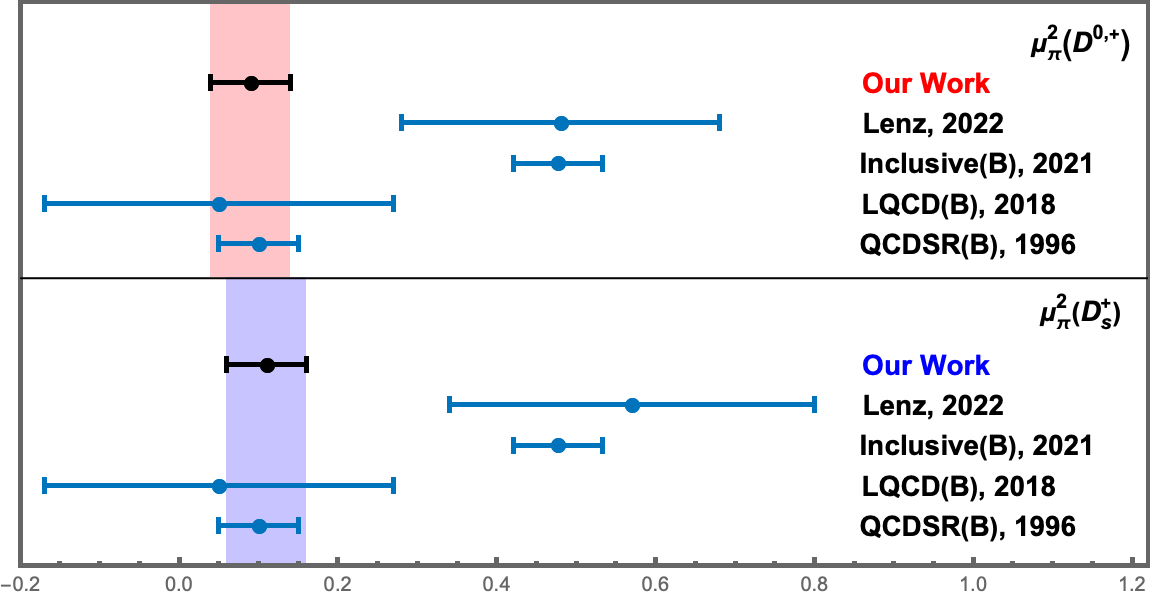
\includegraphics[width=\linewidth]{figures/mupi2.png}
          \caption{非微扰参数$\mu_{\pi}^{2}$的全局拟合估计}
          \label{fig:mupi2}
        \end{minipage}\hfill
        \begin{minipage}{0.494\textwidth}
          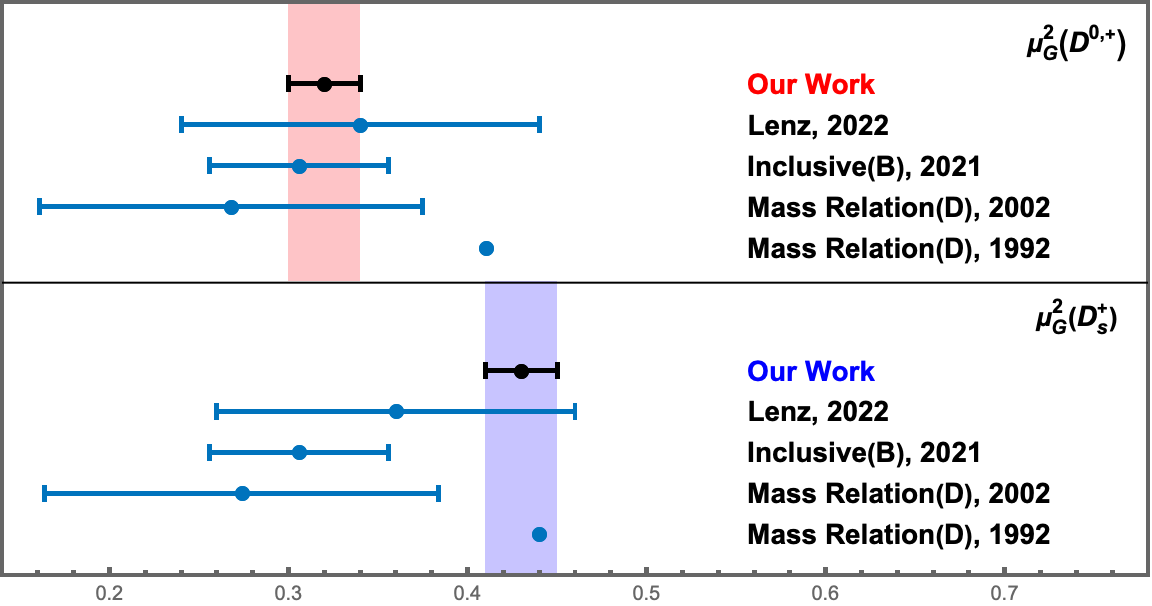
\includegraphics[width=\linewidth]{figures/mug2.png}
          \caption{非微扰参数$\mu_{G}^{2}$的全局拟合估计}
          \label{fig:mug2}
        \end{minipage}
      \end{figure}

    \subsubsection{三. 唯象学分析的结果讨论}
    上节讨论了非微扰参数的全局拟合估计并将其与底介子相关的非微扰矩阵元进行对比。本文在重夸克质量方案的讨论中里给出了1S质量方案下衰变宽度的微扰修正级数，结果表明微扰修正具有良好的收敛行为。进一步，讨论目前拟合结果下的幂次修正展开级数的收敛行为是必要的。
    
    本文将树图水平上量纲三算符对衰变宽度的贡献归一化为一，并逐项讨论各部分修正对衰变宽度的贡献，具体地，
    \begin{equation}
        \begin{aligned}
            \mrm{\Gamma_{sl}^{D^{0,+}}}&\sim 1-0.137-0.055-0.287-0.006 \cdots,\\
            \mrm{\Gamma_{sl}^{D_s^+}}&\sim 1-0.137-0.055-0.385-0.008 \cdots,\\
        \end{aligned}
        \label{eq:decaywidth_1s}
    \end{equation}
    式\eqref{eq:decaywidth_1s}中，从左至右分别是领头阶、次领头阶和次次领头阶的微扰修正和量纲五算符算符矩阵元，量纲六算符矩阵元的幂次修正贡献。无论是幂次修正还是微扰修正，使用本文关于非微扰参数的推荐值，均表现出来良好的收敛性。为了更清楚的展示，对应的贡献如图\ref{fig:D}和\ref{fig:Ds}所示。

\begin{figure}[htbp]
  \centering
  \begin{minipage}{0.5\textwidth}
    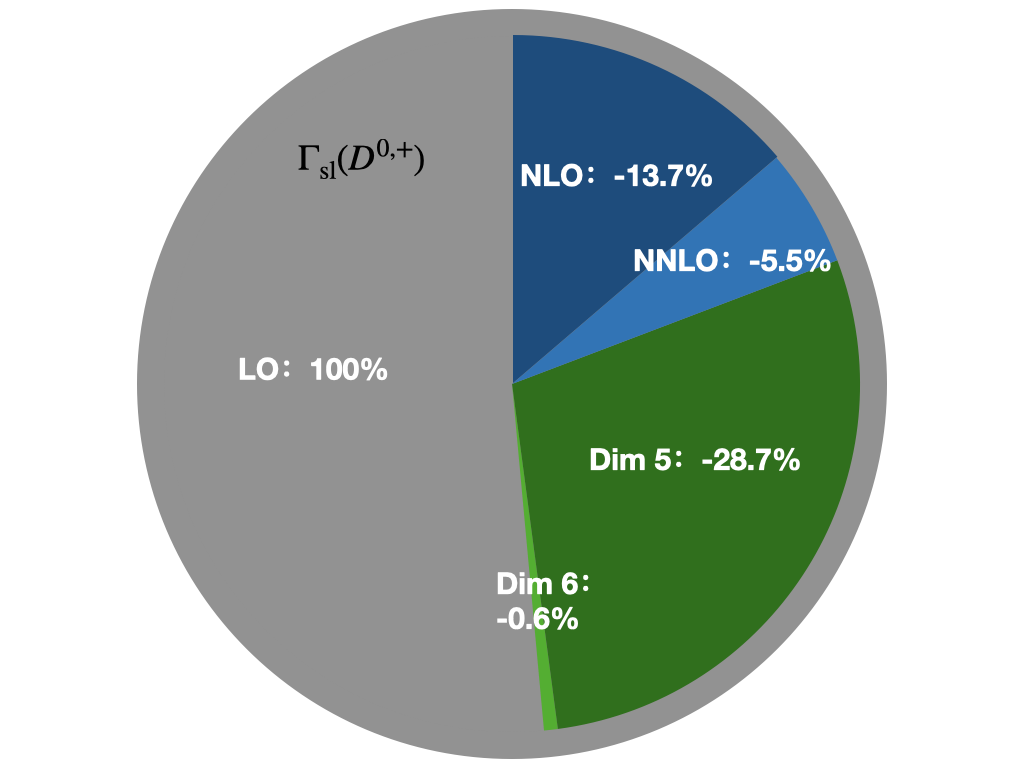
\includegraphics[width=\linewidth]{figures/D.001.png}
    \caption{$\mrm{D^{0,+}}$介子半轻单举衰宽度}
    \label{fig:D}
  \end{minipage}\hfill
  \begin{minipage}{0.5\textwidth}
    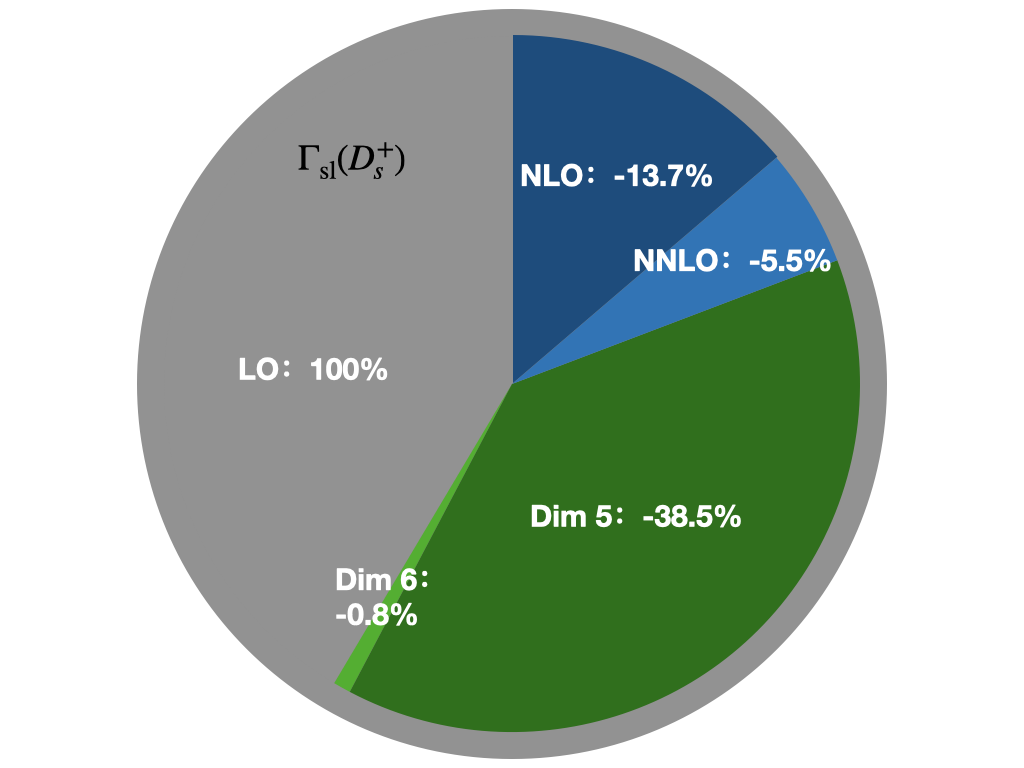
\includegraphics[width=\linewidth]{figures/Ds.001.png}
    \caption{$\mrm{D_s^+}$介子半轻单举衰宽度}
    \label{fig:Ds}
  \end{minipage}
\end{figure}


基于上述讨论，本文推荐在1S 质量方案下计算$\mrm{D}$介子衰变宽度。Alexander Lenz等人计算在$\mrm{D}$介子寿命\ct{King:2021xqp}，他们于重整化能标$\mu= 0.5\GeV$处基于动力学质量方案下给出了三种D介子的衰变宽度对重夸克有效理论中非微扰参数的具体依赖形式。

对于$\mrm{D^{0}}$介子，
\begin{equation}
    \begin{aligned}
    & \Gamma\left(\mrm{D^0}\right)= \Gamma_0[\underbrace{6.15}_{c_3^{\text {Lo }}}+\underbrace{2.95}_{\Delta c_3^{\text {NLO }}}-1.66 \frac{\mu_\pi^2(D)}{\mathrm{GeV}^2}+0.13 \frac{\mu_G^2(D)}{\mathrm{GeV}^2}+23.6 \frac{\rho_D^3(D)}{\mathrm{GeV}^3} \\
    &-1.60 \tilde{B}_1^q+1.53 \tilde{B}_2^q-21.0 \tilde{\epsilon}_1^q+19.2 \tilde{\epsilon}_2^q+\underbrace{0.00}_{\operatorname{dim}-7, \mathrm{VIA}} \\
    &\left.-10.7 \tilde{\delta}_1^{q q}+1.53 \tilde{\delta}_2^{q q}+54.6 \tilde{\delta}_3^{q q}+0.13 \tilde{\delta}_4^{q q}-29.2 \tilde{\delta}_1^{s q}+28.8 \tilde{\delta}_2^{s q}+0.56 \tilde{\delta}_3^{s q}+2.36 \tilde{\delta}_4^{s q}\right] \\
    &= 6.15 \Gamma_0\left[1+0.48-0.13 \frac{\mu_\pi^2(D)}{0.48 \mathrm{GeV}^2}+0.01 \frac{\mu_G^2(D)}{0.34 \mathrm{GeV}^2}+0.31 \frac{\rho_D^3(D)}{0.082 \mathrm{GeV}^3}\right. \\
    &-\underbrace{0.01}_{\operatorname{dim-6,\mathrm {VIA}}}-0.005 \frac{\delta \tilde{B}_1^q}{0.02}+0.005 \frac{\delta \tilde{B}_2^q}{0.02}+0.137 \frac{\tilde{\epsilon}_1^q}{-0.04}-0.125 \frac{\tilde{\epsilon}_2^q}{-0.04}+\underbrace{0.00}_{\operatorname{dim}-7, \mathrm{VIA}} \\
    &-0.0045 r_1^{q q}-0.0004 r_2^{q q}-0.0035 r_3^{q q}+0.0000 r_4^{q q} \\
    &\left.-0.0109 r_1^{s q}-0.0079 r_2^{s q}-0.0000 r_3^{s q}+0.0001 r_4^{s q}\right] .
    \end{aligned}
    \label{eq:decaywidth_D0_kinetic}
    \end{equation}
    为讨论各个部分的贡献，Lenz等人将其归一化至他们采用的中心值上。此外，他们引入$\tilde{B}_i^q = 1 + \delta \tilde{B}_i^q$以表示与真空插入近似的偏差，并且保守地将$\delta \tilde{B}_i^q$归一化为0.02。色八重算符的矩阵元素被归一化为-0.04，除此之外，还引入了比值$r_i^{q q^{\prime}} \equiv \bar{\delta}_i^{q q^{\prime}}/\langle \bar{\delta}_i^{q q^{\prime}}\rangle$表征高量纲算符的误差贡献。
    
    对于$\mrm{D^{+}}$介子，
    \begin{equation}
        \begin{aligned}
        & \Gamma\left(\mrm{D^{+}}\right)= \Gamma_0[\underbrace{6.15}_{c_3^{\mathrm{LO}}}+\underbrace{2.95}_{\Delta c_3^{\mathrm{NLO}}}-1.66 \frac{\mu_\pi^2(D)}{\mathrm{GeV}^2}+0.13 \frac{\mu_G^2(D)}{\mathrm{GeV}^2}+23.6 \frac{\rho_D^3(D)}{\mathrm{GeV}^3} \\
        &-16.9 \tilde{B}_1^q+0.56 \tilde{B}_2^q+84.0 \tilde{\epsilon}_1^q-1.34 \tilde{\epsilon}_2^q+\underbrace{6.76}_{\operatorname{dim}-7} \\
        &\left.-0.06 \tilde{\delta}_1^{q q}+0.06 \tilde{\delta}_2^{q q}-16.8 \tilde{\delta}_3^{q q}+16.9 \tilde{\delta}_4^{q q}-29.3 \tilde{\delta}_1^{s q}+28.8 \tilde{\delta}_2^{s q}+0.56 \tilde{\delta}_3^{s q}+2.36 \tilde{\delta}_4^{s q}\right] \\
        &= 6.15 \Gamma_0\left[1+0.48-0.13 \frac{\mu_\pi^2(D)}{0.48 \mathrm{GeV}^2}+0.01 \frac{\mu_G^2(D)}{0.34 \mathrm{GeV}^2}+0.31 \frac{\rho_D^3(D)}{0.082 \mathrm{GeV}^3}\right. \\
        &-\underbrace{2.66}_{text {dim-6,VIA }}-0.055 \frac{\delta \tilde{B}_1^q}{0.02}+0.002 \frac{\delta \tilde{B}_2^q}{0.02}-0.546 \frac{\tilde{\epsilon}_1^q}{-0.04}+0.009 \frac{\tilde{\epsilon}_2^q}{-0.04}+\underbrace{1.10}_{\operatorname{dim}-7, \mathrm{VIA}} \\
        &-0.0000 r_1^{q q}-0.0000 r_2^{q q}+0.0011 r_3^{q q}+0.0008 r_4^{q q} \\
        &\left.-0.0109 r_1^{s q}-0.0080 r_2^{s q}-0.0000 r_3^{s q}+0.0001 r_4^{s q}\right].
        \end{aligned}
        \label{eq:decaywidth_Dp_kinetic}
        \end{equation}
        其中，由于泡利干涉项的存在，衰变宽度中出现了巨大的负修正；，基于VIA，微扰修正与量纲六、七算符的贡献几乎相互抵消，这表明衰变宽度的展开级数对 $\mrm{\Gamma(D^{+})}$ 对高幂次算符及其QCD修正高度敏感，比如量纲五算符的QCD修正。
        \begin{equation}
            \begin{aligned}
            \Gamma\left(\mrm{D_s^{+}}\right)= & \Gamma_0[\underbrace{6.15}_{c_3^{\mathrm{LO}}}+\underbrace{2.95}_{\Delta c_3^{\mathrm{NLO}}}-1.66 \frac{\mu_\pi^2\left(D_s\right)}{\mathrm{GeV}^2}+0.13 \frac{\mu_G^2\left(D_s\right)}{\mathrm{GeV}^2}+23.6 \frac{\rho_D^3\left(D_s\right)}{\mathrm{GeV}^3} \\
            & -49.6 \tilde{B}_1^s+48.4 \tilde{B}_2^s-13.7 \tilde{\epsilon}_1^s+18.8 \tilde{\epsilon}_2^s+\underbrace{0.63}_{\operatorname{dim-7}} \\
            & \left.-15.8 \tilde{\delta}_1^{q s}+2.34 \tilde{\delta}_2^{q s}+55.4 \tilde{\delta}_3^{q s}+25.0 \tilde{\delta}_4^{q s}\right] \\
            = & 6.15 \Gamma_0\left[1+0.48-0.15 \frac{\mu_\pi^2\left(D_s\right)}{0.57 \mathrm{GeV}^2}+0.01 \frac{\mu_G^2\left(D_s\right)}{0.36 \mathrm{GeV}^2}+0.46 \frac{\rho_D^3\left(D_s\right)}{0.119 \mathrm{GeV}^3}\right. \\
            & -\underbrace{0.20}_{\text {dim-6,VIA }}-0.161 \frac{\delta \tilde{B}_1^s}{0.02}+0.157 \frac{\tilde{B}_2^s}{0.02}+0.089 \frac{\tilde{\epsilon}_1^s}{-0.04}+0.122 \frac{\tilde{\epsilon}_2^s}{0.04}+\underbrace{0.10}_{\text {dim-7,VIA }} \\
            & \left.-0.0064 r_1^{q s}-0.0007 r_2^{q s}-0.0036 r_3^{q s}+0.0012 r_4^{q s}\right]. \\
            &
            \end{aligned}
            \label{eq:decaywidth_Ds_kinetic}
            \end{equation}
        同样的，对于$\mrm{D_s^+}$介子衰变宽度也存在一组收敛性较好的微扰修正展开级数。尽管式\eqref{eq:decaywidth_D0_kinetic},式\eqref{eq:decaywidth_Dp_kinetic}和式\eqref{eq:decaywidth_Ds_kinetic}是基于动力学质量方案下给出的结果，但量纲五算符和量纲六算符的非微扰矩阵元同样起到举足轻重的作用，因此有必要将本文关于非微扰参数的抽取结果带入相关的表达式，粗略定性地展示其对寿命计算的影响。

        事实上，高量纲算符矩阵元的参数化存在模型（近似）依赖，本文将展示在重夸克有效理论求和规则（Heavy Quark Effective Theory SumRule，HQETSR）和真空插入近似两种参数化下有关D介子寿命的理论计算，
        
        Bag参数在HQETSR下的具体数值\ct{Kirk:2017juj}\ct{King:2021jsq}如表\ref{tab:bag_HQETSR}和\ref{tab:bag_HQETSR2}所示，
        \begin{table}
            \scriptsize
            \centering
        \begin{tabular}{|c||c|c|c|c|}
            \hline HQET, $\mu_0=1.5 \mathrm{GeV}$ & $\tilde{B}_1$ & $\tilde{B}_2$ & $\tilde{\epsilon}_1$ & $\tilde{\epsilon}_2$ \\
            \hline$D^{+, 0}$ & $1.0026_{-0.0106}^{+0.0198}$ & $0.9982_{-0.0066}^{+0.0052}$ & $-0.0165_{-0.0346}^{+0.0209}$ & $-0.0004_{-0.0326}^{+0.0200}$ \\
            \hline$D_s^{+}$ & $1.0022_{-0.0099}^{+0.0185}$ & $0.9983_{-0.0067}^{+0.0052}$ & $-0.0104_{-0.0330}^{+0.0202}$ & $0.0001_{-0.0324}^{+0.0199}$ \\
            \hline
            \end{tabular}
            \caption{通过HQETSR计算得到的Bag参数数值结果1}
        \label{tab:bag_HQETSR}
        \end{table}
        \begin{table}
            \scriptsize
            \centering
            \begin{tabular}{|c||c|c|c|c|}
                \hline HQET, $\mu_0=1.5 \mathrm{GeV}$ & $\tilde{\delta}_1$ & $\tilde{\delta}_2$ & $\tilde{\delta}_3$ & $\tilde{\delta}_4$ \\
                \hline$\left\langle D_q\right| \tilde{O}^q\left|D_q\right\rangle$ & $0.0026_{-0.0092}^{+0.0142}$ & $-0.0018_{-0.0072}^{+0.0047}$ & $-0.0004_{-0.0024}^{+0.0015}$ & $0.0003_{-0.0008}^{+0.0012}$ \\
                \hline$\left\langle D_s\right| \tilde{O}^q\left|D_s\right\rangle$ & $0.0025_{-0.0093}^{+0.0144}$ & $-0.0018_{-0.0072}^{+0.0047}$ & $-0.0004_{-0.0024}^{+0.0015}$ & $0.0003_{-0.0008}^{+0.0012}$ \\
                \hline$\left\langle D_q\right| \tilde{O}^s\left|D_q\right\rangle$ & $0.0023_{-0.0091}^{+0.0140}$ & $-0.0017_{-0.0070}^{+0.0046}$ & $-0.0004_{-0.0023}^{+0.0015}$ & $0.0003_{-0.0008}^{+0.0012}$ \\
                \hline
                \end{tabular}
            \caption{通过HQETSR计算得到的Bag参数数值结果2}
            \label{tab:bag_HQETSR2}
        \end{table}
        由于本文未讨论上述非微扰参数估计值之间的关联，因此这里仅讨论D介子衰变宽度理论预言的中心值。本文分析了两种情况，第一种情况对应于D介子衰变宽度的量纲五算符非微扰参数采用本文推荐值，其中非微扰参数使用Lenz等人的推荐值和HQETSR的结果；第二种情况对应于量纲五算符非微扰矩阵元以及量纲六算符的两夸克算符非微扰矩阵元采用本文推荐值，其余非微扰参数采用Lenz等人的推荐值和HQETSR的数值结果。结果如图\ref{fig:HQET}所示。
        \begin{figure}[htbp]
            \centering
            \begin{minipage}{0.5\textwidth}
              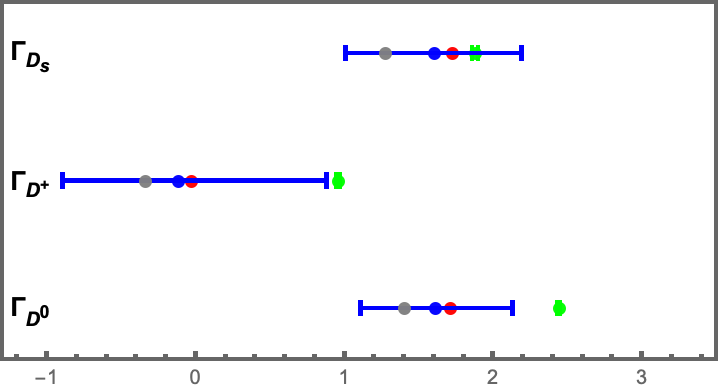
\includegraphics[width=\linewidth]{figures/HQETSR.png}
              \caption{动力学质量方案下基于HQETSR对粲介子衰变宽度的理论预言}
              \label{fig:HQET}
            \end{minipage}\hfill
            \begin{minipage}{0.5\textwidth}
              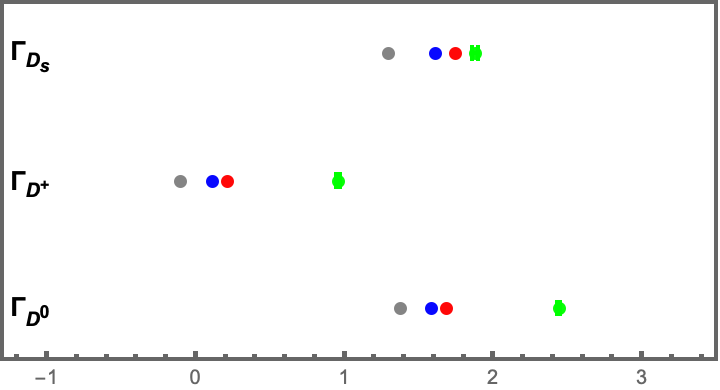
\includegraphics[width=\linewidth]{figures/VIA.png}
              \caption{动力学质量方案下基于VIA对粲介子衰变宽度的理论预言}
              \label{fig:VIA}
            \end{minipage}
          \end{figure}

        图\ref{fig:HQET}中，绿色误差棒表示BESIII合作组和CLEO合作组关于D介子的实验测量值，蓝色误差棒表示Alex Lenz等关于粲介子衰变宽度的理论计算结果，由于$\mrm{D^{+}}$介子中泡利干涉项很大的负贡献导致其理论预言的中心值小于零，且理论预言的误差远远大于实验测量值的误差且其中心值和实验观测量之间存在明显的偏离。红点对应于本文分析的第一种情况，灰点对应于本文分析的第二种情况。红点较之蓝色误差棒更靠近实验观测量值，尤其是$\mrm{D^{+}}$介子，蓝色误差棒的中心值是$-0.15/\text{ps}^{-1}$而红点将这一数值移动至$-0.03/\text{ps}^{-1}$。值得注意的是，对于本文分析的第二种情况，灰点与实验值之间存在更明显的偏离。这表明由于有限的物理可观测量导致无法实现量纲六算符夸克算符非微扰矩阵元的有效拟合估计，另一方面，体现出高幂次修正的重要性。

        此外，本文在动力学质量方案下基于VIA对粲介子寿命进行粗略定性预言，如图\ref{fig:VIA}所示。其中绿色的误差棒表示BESIII合作组和CLEO合作组关于D介子衰变宽度的测量值，蓝点表示Lenz等人基于VIA对粲介子衰变宽度的理论预言，红点对应于本文分析的第一种情况，灰点对应于我们分析的第二种情况。数据点之间的基本特征图\ref{fig:HQET}保持一致。这说明了本文实现了对量纲五算符非微扰矩阵元的有效拟合估计，且实验数据更偏向于本文关于量纲五算符非微扰参数的推荐值。

        不可否认的是，量纲六算符矩阵元的幂次修正贡献同样对粲介子衰变宽度的理论预言起到举足轻重的作用，因此未来关于高幂次算符非微扰矩阵元的QCD修正及其拟合抽取工作是必要的。
\section{本章回顾}
基于第三章关于$\mrm{D}\to X e^{+}\nu$过程的理论分析，本章从两方面介绍了D介子半轻单举衰变的唯象学分析，分别是数据抽取和唯象学分析。
\begin{itemize}
    \item [一] 数据抽取：本文从CLEO合作组$\mrm{D}\to X e^{+}\nu$的实验室系下电子能谱出发利用MC技术抽取出$\mrm{D}^0$和$\mrm{D}^+$介子的衰变宽度，电子能量一、二、三、四阶中心矩的实验观测值，$\mrm{D}_{\mrm{s}}$介子的衰变宽度，电子能量一、二、三、四阶中心矩的抽取来源于BESIII合作组的数据。此外，本文基于关联矩阵和视觉检查实现对该组观测量之间关联程度的讨论，并引入一组新观测量（衰变宽度、电子能量一阶矩与二三四阶中心矩），新观测量将与对应的物理公式一齐参与全局拟合。
    \item [二] 唯象学分析：由于物理可观测量理论公式对粲夸克质量非常敏感，因此本文基于三种质量方案实现重夸克有效理论基本参数的全局拟合抽取；对于幂次修正带来关于非微扰参数拟合估计的误差，本文在三种质量方案的基础上基于两种情形进行全局拟合估计：理论表达式截断于量纲五算符非微扰矩阵元贡献与截断于量纲六算符非微扰矩阵元贡献。对于理论输入参数误差对非微扰参数拟合估计误差的贡献，本文基于MC技术仅讨论了由于重整化能标$\mu$的跑动引起强相互作用耦合常数$\alpha_s(\mu)$的跑动对于非微扰参数拟合估计的误差贡献。
    \item [三] 结果表明：1S质量方案下精确至量纲六算符非微扰矩阵元贡献情形下的平均最小$\chi^2$最小，非微扰参数的拟合估计值没有明显的粲夸克质量方案依赖。
\end{itemize}

本文推荐1S质量方案下精确至量纲六算符非微扰矩阵元贡献情形下的非微扰参数拟合估计值作为唯象学分析的结果，此外，本文基于唯象学分析结果讨论了D介子半轻单举衰变幂次修正和微扰修正的收敛行为，发现在1S质量方案下，D介子半轻单举衰变表现出极好的收敛性。因此本文推荐在1S质量方案下对D介子寿命进行理论计算。
\chapter{夸克质量方案的讨论}
\label{chap:mass_scheme}
\section{引言}
这里写从拉格朗日量出发的巴拉巴拉，引入下面的极质量介绍，当然先简单写一些轻夸克质量方案的介绍，最后介绍对于重夸克质量的naive方案，pole mass方案的简单介绍。

本章的核心问题不是简单比较不同质量方案的定义，而是从 threshold $Q\bar Q$ 体系与静态总能量的物理图像出发，理解 pole mass 的局限、1S/PS 等阈值短距质量的构造逻辑，以及 $\overline{\mathrm{MS}}$ 质量在高能短距过程中的自然性。

\section{极质量方案}
极质量方案基于重夸克自能过程(图\ref{fig:bubble-renormalon})，定义为重夸克在传播子极点处的质量。该定义基于在壳重整化方案，要求修正后的重夸克质量等于物理质量，修正后的电荷等于物理电荷，传播子在极点处的留数等于1，并且在微扰论的逐阶都是well-defined。事实上，夸克质量并不同于电子质量，由于QCD中的夸克禁闭现象，夸克并非渐近态，且QCD的S矩阵在$p^2=m^2$处并不存在夸克极点。这种“非物理性”导致QCD中的极质量不可避免的带有$\mathcal{O}(\Lambda_{QCD})$量级的不确定性，这种不确定性表现为领先的红外重整子的模糊性问题。

\begin{figure}[htbp]
\centering
\begin{tikzpicture}[x=1cm,y=1cm,line cap=round,line join=round]

  \tikzset{
    hq/.style={line width=0.9pt},
    gluon/.style={
      draw,
      decorate,
      decoration={coil,aspect=0.62,segment length=3.0mm,amplitude=1.45mm},
      line width=0.45pt
    },
    dgluon/.style={
      draw,
      dashed,
      decorate,
      decoration={coil,aspect=0.62,segment length=3.0mm,amplitude=1.45mm},
      line width=0.45pt
    },
    bubble/.style={
      circle,
      draw,
      minimum size=0.82cm,
      inner sep=0pt,
      pattern=north east lines,
      pattern color=black,
      line width=0.45pt
    },
    momarrow/.style={
      postaction={
        decorate,
        decoration={
          markings,
          mark=at position #1 with {\arrow{Latex[length=2.6mm,width=1.8mm]}}
        }
      }
    },
    two momarrows/.style args={#1,#2}{
      postaction={
        decorate,
        decoration={
          markings,
          mark=at position #1 with {\arrow{Latex[length=2.6mm,width=1.8mm]}},
          mark=at position #2 with {\arrow{Latex[length=2.6mm,width=1.8mm]}}
        }
      }
    }
  }

  % 外部夸克线（左右各一个 p 箭头）
  \draw[hq,two momarrows={0.12,0.92}] (0,0) -- (8.4,0);
  \node at (1.05,-0.42) {$p$};
  \node at (7.35,-0.42) {$p$};

  % 左侧第一段胶子线（圈动量 k）
  \draw[gluon,momarrow=0.58]
    (1.78,0.00)
    .. controls (1.76,0.30) and (1.84,0.72) ..
    (2.07,1.02);
  \node at (1.35,0.78) {$k$};

  \node[bubble] (B1) at (2.18,1.28) {};

  % 中间虚线胶子
  \draw[dgluon]
    (2.49,1.55)
    .. controls (2.95,2.06) and (3.65,2.34) ..
    (4.30,2.28);

  \node[bubble] (B2) at (4.62,2.20) {};

  % 右侧上方胶子
  \draw[gluon]
    (4.93,1.98)
    .. controls (5.18,1.78) and (5.45,1.50) ..
    (5.67,1.24);

  \node[bubble] (B3) at (5.96,1.16) {};

  % 右侧胶子回到底部夸克线
  \draw[gluon]
    (6.25,0.92)
    .. controls (6.46,0.70) and (6.57,0.34) ..
    (6.52,0.00);

  % 内部夸克传播子（动量 p+k）
  \draw[hq,momarrow=0.63] (1.78,0) -- (6.52,0);
  \node at (4.15,0.34) {$p+k$};

  % 顶点
  \fill[blue] (1.78,0.00) circle (3.4pt);
  \fill[blue] (6.52,0.00) circle (3.4pt);

\end{tikzpicture}
\caption{夸克自能修正图中的链式泡沫图}
\label{fig:bubble-renormalon}
\end{figure}
仿照照量子电动力学中计算电子自能过程的标准技术，最终该图的贡献是
\begin{equation}
    -i \Sigma(\slashed{p})
=
(-i g_s)^2 C_F \mu^{2\epsilon}
\int \frac{d^d k}{(2\pi)^d}\,
\gamma_\mu\,
\frac{i(\slashed{p}+\slashed{k}+m)}{(p+k)^2-m^2+i0}\,
\gamma_\nu\,
\frac{-i g^{\mu\nu}}{k^2+i0}\,.
\label{eq:self-energy}
\end{equation}
以单粒子不可约费曼图为例，对外部动量为 $p$ 的夸克线，取圈动量为 $k$，则内部夸克传播子的动量为 $p+k$。两个夸克——胶子顶点分别贡献因子 $-ig_s\gamma^\mu T^a$，内部夸克传播子贡献
\[
\frac{i(\slashed p+\slashed k+m)}{(p+k)^2-m^2+i0},
\]
在 Feynman 规范下，内部胶子传播子贡献
\[
\frac{-i\,\delta^{ab}g_{\mu\nu}}{k^2+i0}.
\]
再乘上维数正规化下的圈积分测度 $\mu^{2\epsilon}\!\int d^d k/(2\pi)^d$，并将颜色指标收缩为$T^aT^a=C_F,$
便得到式\eqref{eq:self-energy}的具体形式。 
其中 $d=4-2\epsilon$，$\mu$ 是维数正规化中引入的 ’t Hooft 质量尺度\footnote{在维度正规化方案中引入质量尺度$\mu$这一现象同时存在于QED与QCD的单圈自能修正计算过程。原因在于积分维度的改变引起规范耦合常数携带量纲，$\mu$是量纲补偿因子，使得$g_0=\mu^{\epsilon}Z_g g$不携带量纲。$\mu$同时是重整化尺度(量纲为1)，\textbf{物理可观测量若考虑完整的微扰修正，则不应该对$\mu$存在依赖。换而言之，有限阶截断后会保留残余的重整化尺度依赖，这也被用来估计高阶修正不确定性的来源之一}。具体地，若考虑完整微扰修正的物理可观测量$\mathcal{O}$，其不存在对重整化尺度的依赖，因此$\mu\frac{d}{d \mu}\mathcal{O}=0$。对于有限阶微扰修正的截断，该方程并非严格为0，这个不为零的量对应被截断的更高阶修正。换而言之，将某个可观测量写成标准微扰展开形式$O_N(\mu)=\sum_{n=0}^N c_n\left(\ln \frac{\mu}{Q}\right) \alpha_s^{n+p}(\mu)$, $p$是该观测量的微扰展开从$\alpha_s$的第几阶出现，其精确结果不存在对重整化尺度的依赖。但对于有限阶修正，其满足$\mu \frac{d}{d \mu} O_N=\mathcal{O}\left(\alpha_s^{N+p+1}\right)$.该方程说明，对于有限阶截断的物理可观测量，其对重整化尺度的敏感性本身就是”下一阶乃至更高阶未算项“。因此对重整化尺度在某个合理区间里遍历取值得到物理可观测量的数值改变，自然可以被拿来作为 missing higher orders 修正的经验估计，也就是所谓的 \textbf{renormalization scale variation}}。

对于式\eqref{eq:self-energy},假设外部动量$p$接近于夸克质量$m$，即on-shell条件成立，讨论软贡献区域，即$k^\mu$远小于m，则此时的重夸克传播子具有eikonal近似形式
$$
\frac{1}{(p+k)^2-m^2+i 0} \rightarrow \frac{1}{2 m v \cdot k+i 0}
$$
在该近似下，式\eqref{eq:self-energy}的软贡献可以被重写为
$$
\Delta m_{\mathrm{soft}} \sim \int \frac{d^d k}{(2 \pi)^d} \frac{1}{k^2} \frac{1}{v \cdot k}\sim\int k^3 \frac{1}{k^3}dk \sim \int_0^\mu d k \text { (constant) }
$$
分子在$k\to 0$极限下没有奇异项，仅贡献常数或者k趋于0的高阶修正。因此这里仅讨论分母。红外区域给出的是IR的线性依赖，后面再讨论泡泡链的修正后，会有$\Delta m_{\mathrm{IR}}^{(n)} \sim \int_0^\mu d k \ln ^n\left(\frac{k^2}{\mu^2}\right)$的贡献。

以上是关于单胶子泡泡图的简单说明，对于多胶子链式泡泡图，首先关注泡泡之间的传播子连接，一般意义上的胶子传播子具有如下的形式
$$
D_{\mu \nu}^{(0)}(k)=\frac{-i}{k^2}\left(g_{\mu \nu}-(1-\xi) \frac{k_\mu k_\nu}{k^2}\right) .
$$
将泡泡的动力学信息编码为$\Pi$,则插入一个泡，会有$D^{(0)}\Pi D^{(0)}$，插入两个泡会有$D^{(0)}\Pi D^{(0)}\Pi D^{(0)}$，以此类推，最终链式泡泡图的贡献可以被重写为
$$
D=D^{(0)}+D^{(0)} \Pi D^{(0)}+D^{(0)} \Pi D^{(0)} \Pi D^{(0)}+\cdots
$$
形式上根据Dyeson级数求和可并展开为几何级数,
$$D=\frac{D^{(0)}}{1+\Pi(k^2)}=D^{(0)}\sum_{M=0}^{\infty}[-\Pi(k^2)]^N$$
对于泡泡$\Pi_{k^2}$,由规范对称性和横向极化要求，$\Pi_{k^2}$具有如下的结构
$$\Pi_{\mu \nu}(k)=\left(k_\mu k_\nu-k^2 g_{\mu \nu}\right) \Pi\left(k^2\right),$$
表明该无量纲标量函数$\Pi(k^2)$在无质量极限下(大$n_f$极限下)，圈积分唯一的尺度依赖是$k^2$。根据标准圈图计算结果，通过量纲分析，可知$\Pi(k^2)$具有如下的一般结构
\begin{equation}
\Pi\left(k^2\right)=\frac{\alpha_s}{4 \pi}\left[\text { divergence }+ \text { const }+c \ln \frac{-k^2}{\mu^2}\right] .
\end{equation}
该圈积分的贡献只与对数项和一个重整化方案依赖的常数项相关。最终该含有N个泡泡的图会给出$\ln^{N}(-k^2/\mu^2)$的项.

在散射振幅的水平，胶子传播子往往和两个有效顶点耦合在一起，形成一个有效的耦合常数，记为$\alpha_s(k^2)$，
\begin{equation}
  \alpha_s(k^2)=\frac{g_s^2}{1+\Pi(k^2)}\propto \frac{g_s^2}{1+\frac{\beta_0 \alpha_s}{4 \pi} \ln \frac{k^2}{\mu^2}}+\cdots,
  \label{eq: alphas_running}
\end{equation}

此外，$\alpha_s$随尺度$\mu$的变化由重整化群方程描述，$\mu \frac{d\alpha_s}{d\mu}=\beta$,单圈水平下该方程的解是
$\alpha_s(k^2)=\alpha_s(\mu^2)/(1+\beta_0 \alpha_s(\mu^2)/(4 \pi) \ln(k^2/\mu^2))$

泡泡链重求和产生的传播子修正与重整化群方程的一圈解呈现相同的对数结构，因此可以将其理解为耦合常数重整化群跑动的图像化体现\cite{Papavassiliou_1997}。

通过引入跑动耦合常数$\alpha_s(k)$，质量位移的软贡献可以重新写为：
\begin{equation}
  \Delta_{\mathrm{soft}} \sim K\int_{0}^{\mu} \alpha_s(k) dk, 
\end{equation}
其中K是可计算的常数，比如在$\overline{\text{MS}}$方案下，$K=C_{F} e^{5/6}/\pi$.
\subsection{Renormalon: 阶乘增长 ,Borel变换与模糊性}
事实上，pole mass在定义在极点处，微扰论意义上是逐阶良定义的，但依然存在软贡献区域存在线性的IR敏感性，表现为阶乘形式的增长。
将式\eqref{eq: alphas_running}按照几何级数在软贡献区域进行展开，有$$\alpha_s(k)=\alpha_s(\mu) \sum_{n=0}^{\infty}\left[\beta_0 \alpha_s(\mu) \ln \left(\mu^2 / k^2\right)\right]^n$$.质量位移计算结果可改写为
$$
\Delta m_{\mathrm{soft}} \sim K \sum_{n=0}^{\infty} \alpha_s^{n+1}(\mu) \beta_0^n \int_0^\mu d k \ln ^n\left(\mu^2 / k^2\right)
$$
该结果对应的特征积分是$I_n=\int_0^\mu d k \ln ^n\left(\mu^2 / k^2\right)$, 做如下的变量代换，有
$$
t=\ln (\mu / k) \Rightarrow k=\mu e^{-t}, d k=-\mu e^{-t} d t
$$
$I_n$可以被重写为
\begin{equation}
  \boxed{
I_n=\mu \int_0^{\infty} d t e^{-t}(2 t)^n=\mu 2^n \Gamma(n+1)=\mu 2^n n!}
\label{eq: chatacter_Integral}
\end{equation}
因此，质量位移的软贡献具有阶乘增长的行为\cite{Bigi:1994em}。以$\overline{\text{MS}}$质量方案为例，最终得到的质量位移结果具有如下的结\cite{Beneke:2021lkq}
\begin{equation}
m_{\mathrm{pole}}-m_{\overline{\mathrm{MS}}}(\mu)=\frac{C_F e^{5 / 6}}{\pi} \mu \sum_{n \geq 0}\left(2 \beta_0\right)^n n!\alpha_s^{n+1}(\mu),
\end{equation}

Borel变换将阶乘增长的级数转换为Borel平面的奇点结构（如图\ref{fig:borel_plane_adler_pretty}所示），从Borel平面可直接读出渐进级数为什么发散，来自什么物理区域的贡献，以及对应什么量级的不确定性，这也是引入Borel变换的动机。
\begin{figure}[htbp]
\centering
\begin{tikzpicture}[scale=1.05, >=stealth]

    % axes
    \draw[->, thick] (-0.8,0) -- (8.2,0) node[right] {$\mathrm{Re}\,u$};
    \draw[->, thick] (0,-2.2) -- (0,2.6) node[above] {$\mathrm{Im}\,u$};

    % branch points and cuts
    \foreach \x/\lab in {1.5/{\frac12},3.2/{\frac32},4.9/{\frac52},6.6/{\frac72}}{
        % branch point
        \filldraw[black] (\x,0) circle (2.2pt);
        % cut to the right
        \draw[thick] (\x,0) -- (\x+0.85,0);
        % label
        \node[below=5pt] at (\x,0) {$u=\lab$};
    }
    % title-like annotation
    \node[align=left] at (6.6,1.8)
    {IR renormalons of pole mass};
\end{tikzpicture}
\caption{Pole mass 在 Borel \(u\)-平面上的 IR renormalon 解析结构示意图。黑点表示 branch points 的起点；从这些点向右延伸的线段表示相应的 branch cuts。}
\label{fig:pole_mass_borel_branch}
\end{figure}

具体地，定义Borel变换为$B[R](t)=\sum_{n=0}^{\infty} \frac{r_n}{n!}t^n$, 若$r_n=K a^n\Gamma(n+1+b)$,则
$$
B[R](t) \sim \frac{K \Gamma(1+b)}{(1-a t)^{1+b}} .
$$
若$B[R](t)$在正实轴没有奇点，且在无穷远处增长足够慢，则在形式上可定义Borel积分\footnote{这里的$\alpha$是微扰展开参数}，
\begin{equation}
R_{\rm Borel}(\alpha)=\int_{0}^{\infty}dt\,e^{-t/\alpha}B[R](t).
\end{equation}
如果 Borel 奇点落在正实轴上，那么 Borel 积分绕奇点上、下侧定义时会给出不同结果，从而产生歧义。这个歧义通常表现为
\begin{equation}
  \text{Im} R_{\rm Borel}=\mp(\pi K/a) e^{-1/(a\alpha)}(a\alpha)^{-b}.
\end{equation}
其中的正负号取决于积分路径位于正实轴的上侧还是下侧，极质量定义中的歧义性也反映在\textbf{Borel积分路径的歧义性}上，该路径积分的差异会给出一个非微扰的指数量级不确定性\footnote{对于式\eqref{eq: chatacter_Integral},a=2,b=0, 对于质量位移结果，部分经典文献中，将t重定义为u，即该积分在u=1/2处存在奇点。}。

设某物理量 $R(Q)$ 的 Borel 变换在正实轴上存在 IR renormalon 奇点 $u=u_0>0$。
则 Borel 积分的歧义一般具有形式
\[
\delta R \sim e^{-u_0/((-b_0)\alpha_s(Q))}.
\]
利用一圈 running coupling
\[
\alpha_s(Q)=\frac{1}{-b_0\ln(Q^2/\Lambda_{\rm QCD}^2)},
\]
可得
\[
e^{-u_0/((-b_0)\alpha_s(Q))}
=
e^{-u_0\ln(Q^2/\Lambda_{\rm QCD}^2)}
=
\left(\frac{\Lambda_{\rm QCD}^2}{Q^2}\right)^{u_0}.
\]
因此，位于 $u=u_0$ 的 IR renormalon 对应的非微扰歧义量级为
\[
\delta R(Q)\sim \left(\frac{\Lambda_{\rm QCD}^2}{Q^2}\right)^{u_0},
\]
再乘以 $R$ 自身的质量维数所需的硬标度因子。
对于 pole mass 而言，首个 IR renormalon 位于 $u_0=\frac12$，且
$m_{\rm pole}-m_{\overline{\rm MS}}$ 具有质量维数 1，
故
\[
\delta m_{\rm pole}\sim Q\left(\frac{\Lambda_{\rm QCD}^2}{Q^2}\right)^{1/2}
\sim \Lambda_{\rm QCD}.
\]
pole mass 定义上存在$\mathcal{O}(\Lambda_{\rm QCD})$的模糊性便来自leading阶的renormalon\footnote{对于 renormalon 奇点，需要区分奇点位置与奇点附近的局部结构。

\begin{itemize}
    \item 奇点位置 $u=u_0$ 由红外或紫外区域的幂次行为决定，而不由更高阶 running coupling 决定。
    一般地，若小动量区行为为$F(k^2)\sim k^a$,
    则对应的 IR renormalon 位置为
    $
    u_0=\frac{a}{2}.
    $
    \item 更高阶 RG 信息（如两圈、三圈 $\beta$ 函数）不会改变 $u_0$，而只会把 simple pole 改成 branch point，
    即把
    $
    \frac{1}{1-u/u_0}
    $
    修正为
    \[
    \frac{1}{(1-u/u_0)^{1+b}}
    \left[1+c_1(1-u/u_0)+c_2(1-u/u_0)^2+\cdots\right].
    \]
\end{itemize}}。

Subleading阶的renormalon会带来更高幂次的$\Lambda_{\rm QCD}$依赖，但对于pole mass而言，leading阶的$\mathcal{O}(\Lambda_{\rm QCD})$不确定性已经足以说明其定义上的模糊性问题\cite{Beneke:1998ui}。
\section{阈值质量方案：1S质量方案}
1S质量方案并非对极点质量的任意重命名，而是从非相对论 $Q \bar{Q}$ 阈值动力学中抽取出的短距质量。它定义为「虚构」$1^3 S_1$ 夸克偶素基态微扰质量的一半，因此天然吸收了总静能 $2 m_{\text {pole }}+V_{\text {stat }}$ 中的物理可控部分。由于 pole mass 的 $O\left(\Lambda_{Q C D}\right)$ 红外重整子与静态势中的对应长程修正在总静能中相互抵消， 1S质量方案也随之摆脱了极点质量方案中的领头红外重整子任意性。它适合描述 $q\bar{q}$ 等阈值过程；当将其用于单举衰变时，需要基于形式展开参数$\epsilon$进行来保证与极点质量方案中扰级数之间的红外敏感项逐阶一致地重组与对消。
\subsection{从单胶子交换到pNRQCD的静态势物理图像}


\subsection{1S质量方案}
    这里写如何规避红外重整子任意性问题，
\subsection{Upsilon Expansion}
A. H. Hoang等人在上世纪末本世纪初对于1S质量方案进行了系统的研究，提出了1S质量方案的定义和计算方法，并将其应用于顶夸克质量的衰变过程。通过修饰的微扰展开对$\alpha_s$进行重求和以消除固定阶的「红外重整子任意性问题」，具体地，将其用于inclusive decay之类的“硬过程”时，必须使用upsilon expansion，使非微扰束缚能级数与普通过程的微扰级数正确配对。
对于顶夸克的阈值对产生过程，1S质量方案提供了一个自然的框架来定义和计算顶夸克的质量。一个比较系统完整的质量转换关系被提出，并且在数值上展示了极好的收敛性(hep-ph/9904468(78))\cite{Hoang:1999zc}。

\begin{equation}
\begin{aligned}
M_{1 S}= & M_t-\epsilon \frac{M_t C_F^2 a_s^2}{8} \\
& -\epsilon^2 \frac{M_t C_F^2 a_s^2}{8}\left(\frac{a_s}{\pi}\right)\left[\beta_0(L+1)+\frac{a_1}{2}\right] \\
& -\epsilon^3 \frac{M_t C_F^2 a_s^2}{8}\left(\frac{a_s}{\pi}\right)^2\left[\beta_0^2\left(\frac{3}{4} L^2+L+\frac{\zeta_3}{2}+\frac{\pi^2}{24}+\frac{1}{4}\right)+\beta_0 \frac{a_1}{2}\left(\frac{3}{2} L+1\right)\right. \\
& \left.\quad+\frac{\beta_1}{4}(L+1)+\frac{a_1^2}{16}+\frac{a_2}{8}+\left(C_A-\frac{C_F}{48}\right) C_F \pi^2\right],
\end{aligned}
\label{eq:OS_to_1S_NNNLO}
\end{equation}
其中$L=\ln \left(\mu/\left(C_F a_s M_t\right)\right)$，$\epsilon$是upsilon expansion的形式展开参数，用于标记QCD微扰展开的阶数。具体地，微扰级数中的$\mathcal{O}(\alpha_s^N)$项被赋予$\epsilon^N$，而极质量到1S质量转换关系中的$\mathcal{O}(\alpha_s^N)$（除去对数项）则被视为$\epsilon^{N-1}$;按$\epsilon$重新展开并截断到固定阶后，最终再令该参数取1，在技术上以完成重求并实现消除红外重整子任意性问题的目的。
注意到，$M_{1S}/M_t$相对于1的偏离始于$\epsilon$的线性项，即$\mathcal{O}(\epsilon \alpha_s^2)$，此外，L的出现始于$\epsilon$的平方项。换而言之，$M_{t}=M_{1S}(1+\delta)$且$\delta \sim \mathcal{O}(\epsilon \alpha_s^2)$。代入L的表达式并展开至$\epsilon$的线性项，我们可以得到
\begin{equation}
    L=\ln \left(\mu/\left(C_F a_s M_t\right)\right)=\ln\left(\mu/\left(C_F a_s M_{1S}\right)\right)-\ln\left(1+\delta\right)=\ln\left(\mu/\left(C_F a_s M_{1S}\right)\right)-\delta+\frac{\delta^2}{2}+\mathcal{O}(\delta^3)
\end{equation}
若$L_{1S}$与$L_{OS}$的差异在$\mathcal{O}(\epsilon^n)$量级,则该差异出现于式\eqref{eq:OS_to_1S_NNNLO}中的$\epsilon^{n-1}$项,因此，$L_{1S}$与$L_{OS}$的差异对于$\mathcal{O}(\epsilon^{n-1})$的微扰级数展开截断而言可以忽略。

对于具体物理观测量中的质量方案的幂次分析的讨论，则需要根据具体的物理过程和观测量来进行分析。例如对于精确至两圈图水平微扰修正的D介子单举半轻衰变过程的衰变宽度如下：
\begin{equation}
\begin{aligned}
    \Gamma_{D_{i}} = \sum_{q = \mathrm{d}, \mathrm{s}} \hat{\Gamma}_0 \mrm{\left| V_{\mathrm{c}q} \right|^2} m_{\mathrm{c}}^5 \Big\{ 1 & + \frac{\alpha_s}{\pi} \frac{2}{3} \left( \frac{25}{4} - \pi^2 \right)\\
    & + \frac{\alpha_s^2}{\pi^2} \left[ \frac{\beta_0}{4} \frac{2}{3} \left( \frac{25}{4} - \pi^2 \right) \log \left( \frac{\mu^2}{m_{\mathrm{c}}^2} \right) + 2.14690 n_l - 29.88311 \right]\\  
    &- 8 \rho \delta_{\mathrm{s}q} - \frac{1}{2} \frac{\mu_{\pi}^{2}(D_{i})}{m_{\mathrm{c}}^2} - \frac{3}{2} \frac{\mu_{\mathrm{G}}^{2}(D_{i})}{m_{\mathrm{c}}^2} + 6 \frac{\rho_{\mathrm{D}}^3\left(D_{i}\right)}{m_{\mathrm{c}}^3} + \dots \Big\},
\end{aligned}
\label{eq:decaywidth-mass-scheme}
\end{equation}
我们以截断至NNNLO的贡献为例进行说明：对数项$\ln(\mu^2/m_{c}^2)$出现于$\alpha_s^2$项，则该对数项对于upsilon expansion展开级数的贡献始于$\mathcal{O}(\epsilon^2)$量级，因此方便起见可对该对数项单独进行质量方案的转换，仅需对质量转换公式精确至$\mathcal{O}(\delta^2)$，即保留至$\mathcal{O}(\epsilon \alpha_s^2)$量级即可\footnote{这里讨论对应的三个问题分别是：1. 能否把式\eqref{eq:OS_to_1S_NNNLO}
里L中的$M_{t}$直接换成$M_{1S}$; 2. 为什么代码中物理观测量里的log项没有直接应用质量转换公式而是保留了$1+\delta$的线性项之后再统一做$\epsilon$展开；3. 在1S质量方案下，NNNLO截断对应于什么样的丢弃规则。}。
\section{阈值减除质量方案: PS质量方案}
\section{标准UV短矩质量：$\bar{\text{MS}}$质量方案}
\section{不同质量方案的对比}
\newpage
\section{补充计算}
\subsection{不同重整化方案下质量位移的一般性结果}
本小节主要从重整化后的自能图出发，计算不同重整化方案下质量位移的一般结果，并进行简单讨论。对于重整化后的费米子两点函数，传播子的极点位置定义了所谓的 \emph{pole mass}。  
设重整化后的逆传播子为
\begin{equation}
S_R^{-1}(p)=\slashed p-m-\Sigma(\slashed p),
\end{equation}
其中 \(m\) 是某个给定重整化方案下的质量参数，\(\Sigma(\slashed p)\) 是重整化后的自能。

我们关心的问题是：

\begin{itemize}
    \item 如何由 \(\Sigma(\slashed p)\) 定义传播子的极点位置 \(m_{\rm pole}\)；
    \item 如何在一阶精度下导出
    \begin{equation}
    \delta m \equiv m_{\rm pole}-m
    =\frac{1}{4m}\text{Tr}[(\slashed p+m)\Sigma(\slashed p)]|_{p^2=m^2}
    +\mathcal{O}(\Sigma^2);
    \end{equation}
\end{itemize}
由洛伦兹协变性可知，在真空中的费米子二点函数只能依赖于 \(p^\mu\)，因此 \(\Sigma(\slashed p)\) 的最一般狄拉克结构只能由
$\mathbf{1},  \slashed p$两种\footnote{若理论本身宇称不守恒，且额外存在背景场，则需要重新讨论来自洛伦兹对称性的约束}。故可写为
\begin{equation}
\Sigma(\slashed p)=A(p^2)\,\slashed p+B(p^2)\,m,
\end{equation}
其中 \(A(p^2)\) 与 \(B(p^2)\) 都是无量纲函数。

传播子的极点位置由$\det S_R^{-1}(p)\Big|_{p^2=m_{\rm pole}^2}=0$定义。
等价地，也可以说在壳上存在旋量 \(u(p)\)，满足
\begin{equation}
S_R^{-1}(p)\,u(p)=0,
\qquad p^2=m_{\rm pole}^2.
\end{equation}

代入逆传播子的表达式，
\begin{equation}
\Big[
\bigl(1-A(p^2)\bigr)\slashed p
-
\bigl(1+B(p^2)\bigr)m
\Big]u(p)=0.
\end{equation}
在壳上满足\footnote{$S^{-1}\sim Z_2^{-1}(\slashed{p}-m_{\text{pole}} )+ \mathcal{O}(p^2-m_{\text{pole}}^2)$}
\begin{equation}
\slashed p\,u(p)=m_{\rm pole}\,u(p),
\end{equation}
因此可得到标量条件
\begin{equation}
\bigl(1-A(m_{\rm pole}^2)\bigr)m_{\rm pole}
-
\bigl(1+B(m_{\rm pole}^2)\bigr)m=0.
\end{equation}

定义
\begin{equation}
m_{\rm pole}=m+\delta m,
\qquad
\delta m=\mathcal{O}(\Sigma).
\end{equation}
由于 $A, B\sim \mathcal{O}(\Sigma)$ ，因此在一阶精度下，
\begin{equation}
A(m_{\rm pole}^2)=A(m^2)+\mathcal{O}(\Sigma^2),
\qquad
B(m_{\rm pole}^2)=B(m^2)+\mathcal{O}(\Sigma^2).
\end{equation}
因此标量条件在一阶精度下变成
\begin{equation}
\bigl(1-A(m^2)\bigr)(m+\delta m)-\bigl(1+B(m^2)\bigr)m=0
+\mathcal{O}(\Sigma^2).
\end{equation}
展开并整理后得到
\begin{equation}
\delta m
=
m\bigl[A(m^2)+B(m^2)\bigr]+\mathcal{O}(\Sigma^2).
\end{equation}
A和B是属于自能图的狄拉克结构的系数，可以凭此得到质量位移结果对自能图的依赖的一般性表达式。

使用正能投影算符$\slashed{p}+m$对自能图进行投影，并取迹，可以得到
\begin{equation}
\text{Tr}[(\slashed p+m)\Sigma(\slashed p)]|_{p^2=m^2}=4 p^2 A(m^2)+4 m^2 B(m^2)=4 m^2 \bigl[A(m^2)+B(m^2)\bigr].
\end{equation}
最终得到质量位移的一般计算结果
\begin{equation}
\boxed{
\delta m
=
\left.\frac{1}{4m}\text{Tr}\!\big[(\slashed p+m)\Sigma(\slashed p)\big]\right|_{p^2=m^2}
+\mathcal{O}(\Sigma^2)
}.
\label{eq: massdistance}
\end{equation}
该结果表明，质量位移 $\delta m$ 可以通过对自能图 $\Sigma(\slashed p)$ 进行特定的投影和取迹来计算\footnote{利用狄拉克代数的性质，使用求迹操作将质量位移相关的标量部分投影出来}, \textbf{式\eqref{eq: massdistance}的结构无重整化方案依赖}，因为它仅取决于：1. 自能图的狄拉克结构, 2. 极点条件: $S^{-1}u(p)=0$, 3. 自能修正的一阶展开。比如式\eqref{eq: massdistance}中的m是$\overline{\mathrm{MS}}$质量，$\Sigma$是$\overline{\mathrm{MS}}$方案下的自能图，那么式\eqref{eq: massdistance}就给出了$\overline{\mathrm{MS}}$质量与极点质量之间的关系。若m是极质量，则按照定义，$\delta m=0$，因此式\eqref{eq: massdistance}也给出了极质量方案下自能图的特定投影必须为零的条件。

传播子在极点附近应具有如下形式：
\begin{equation}
S_R(p)\xrightarrow[p^2\to m_{\rm pole}^2]{}
\frac{i\,Z_2^{\rm pole}}{\slashed p-m_{\rm pole}+i0}
+\text{regular}.
\end{equation}
这里 \(Z_2^{\rm pole}\) 是极点留数。若选择 OS 方案，则通常要求极点留数归一化为 \(1\)。这意味着：

\begin{itemize}
    \item 极点确实位于 \(p^2=m_{\rm pole}^2\)；
    \item 极点前的系数被规范为单位留数。
\end{itemize}

这两个条件共同决定了 OS 方案中的质量 counterterm 与波函数重整化常数。

从逆传播子的角度看，第一条是
\begin{equation}
S_R^{-1}(p)\,u(p)=0
\qquad \text{at }\slashed p=m_{\rm pole},
\end{equation}
而第二条则对应于在极点附近对 \(S_R^{-1}(p)\) 对 \(\slashed p\) 或 \(p^2\) 的一阶展开系数施加归一化条件。

在 OS（on-shell）方案中，重整化条件直接要求：

\begin{itemize}
    \item 重整化后的传播子极点位于物理质量 \(m_{\rm pole}\)；
    \item 极点留数为 \(1\)。
\end{itemize}

因此 OS 方案下的质量参数就是 pole mass：
\begin{equation}
m_{\rm OS}=m_{\rm pole}.
\end{equation}
这意味着自能中的相应修正被完全吸收到极点位置里。

但是在 QCD 中，pole mass 对软动量区域敏感，因此会带有长程红外敏感性\footnote{我们质量位移结果的红外结果进行量级分析时，需要在ekional 近似下进行讨论。此时式\eqref{eq: massdistance}的分子部分以及求迹操作仅会贡献到常数因子，不参与红外结构的分析}。具体地，
\begin{equation}
\delta m_{\mathrm{soft}} \sim \int \frac{d^d k}{(2 \pi)^d} \frac{1}{k^2} \frac{1}{v \cdot k} \sim \int k^3 \frac{1}{k^3} d k \sim \int_0^\mu d k \text { (constant) }\sim \mathcal{O}(\Lambda_{\rm QCD})
\end{equation}
\textbf{
一般地，重整化后的逆传播子可写为
\[
S_R^{-1}(\slashed p)=\slashed p-m-\Sigma(\slashed p).
\]
在 OS 重整化方案中，质量参数被定义为传播子的极点位置，因此
\[
S_{\rm OS}^{-1}(\slashed p)\big|_{\slashed p=m_{\rm pole}}=0,
\]
也就是说，自能修正对极点位置的贡献被完全吸收到 pole mass 的定义中，其中也包括软胶子的贡献。正因如此，pole mass 对红外区域敏感，从而具有$
\mathcal O(\Lambda_{\rm QCD})
$量级的本征不确定性。}
\chapter{总结与展望}
寻找新物理和理解QCD非微扰是目前粒子物理领域内的核心任务。而粲物理，特别是粲味强子弱衰变对于这两个核心任务起到关键作用：一方面，此类过程作为弱衰变，对可能存在的高能标新物理非常敏感，另一方面，过程中初末态强子化由非微扰 QCD 所主导，是探究 QCD的重要平台。粲味强子弱过程分为遍举衰变和单举衰变，后者理论研究方法比较成熟，可以从第一性原理出发系统的求解幂次修正的形式，因而其理论误差更加可控。相比于B介子和底重子，由于粲夸克质量较小，按QCD耦合常数展开的微扰修正以及按重夸克质量负幂次展开的幂次修正都更加显著，因此粲味强子弱衰变为研究高阶修正提供了更加理想的环境。因此粲味强子单举衰变的研究具有其独特意义。

与此同时，粒子物理领域内长期存在一些疑难与反常，并引起领域内的广泛关注。对于更清楚的认识甚至解决这些疑难，粲味强子单举衰变的研究可以起到关键性的作用。其中之一是粲强子寿命的理论预言与实验测量不一致，原因在于寿命理论计算依赖非微扰参数，目前理论工作中的非微扰参数均有较大的模型依赖。因此，基于粲味强子举衰变过程的观测量和对应实验数据，实现对非微扰矩阵元模型无关的抽取，是理解甚至解决粲强子寿命疑难的关键所在。

本文在以下三个方面对理解粲强子寿命疑难进行了努力：

首先理论上，基于重夸克有效理论和算符乘积展开，讨论高阶修正对非微扰强子矩阵元的影响。高阶修正主要包括重夸克质量负幂次展开的幂次修正和QCD耦合常数展开的微扰修正。关于重夸克质量负幂次展开的幂次修正，介绍了$\mrm{B\to X_{c}e\nu}$过程树图水平量纲三和量纲五算符对应结构函数的匹配与相空间解析积分，得到对应的电子能谱解析形式。在此基础上，通过取末态粲夸克质量趋于零的极限，可得$\mrm{B\to X_{u}e\nu}$过程树图水平的电子能谱解析形式。关于QCD耦合常数展开的微扰修正，在单圈水平上，本文介绍了$\mrm{B\to X_{c}e\nu}$过程的结构函数，并通过取末态粲夸克质量趋于0的极限，得到$\mrm{B\to X_{u}e\nu}$过程的结构函数，在此基础上，对相空间进行解析积分，得到对应的电子能谱解析形式。将上述的电子能谱转换到粲夸克半轻单举衰变过程中，即得到$\mrm{D\to X e^{+}\nu}$过程电子能谱的解析形式。由于重夸克有效理论的局限性，需要对电子能谱进行相空间加权积分进行“平滑”处理后，方可与实验观测量进行对比。本文讨论了$\mrm{D\to X_s e^{+}\nu}$和$\mrm{D\to X_d e^{+}\nu}$两类过程，粲强子半轻单举衰变的末态夸克包括奇异夸克，其质量接近非微扰能标，因此需要作为软自由度进行保留，对于$\mrm{D\to X_s e^{+}\nu}$，末态奇异夸克的质量效应被考虑在内。基于$\mrm{D\to X e^{+}\nu}$过程的电子能谱，通过对其做相空间加权解析积分，给出关于衰变宽度、电子能量原点矩的理论表达式，它们依赖于非微扰强子矩阵元。

实验上，美国的CLEO合作组2009年测量了实验室系下三种D介子半轻单举衰变过程的电子能谱，我国的BESIII合作组于2018年更新了$\mrm{D_s^+}$介子半轻单举衰变过程的电子能谱。本文从粲介子半轻单举衰变的电子能谱出发，利用重夸克有效理论的预言，在红外区域对其做拟合外推；关于系统误差，对衰变分支比的系统误差进行延拓并假设每个bin的系统误差全关联，最终得到实验室系下完整的电子能谱。基于此，对其做关于电子能量的加权求和得到电子能量矩和衰变宽度的实验测量值。除此之外，还讨论了电子能量矩之间的关联系数，最终选择衰变宽度，电子能量一阶原点矩，电子能量第二、三和四阶中心矩作为数据点与对应的理论表达式一齐进行全局拟合。

唯象学分析上，由于衰变宽度对粲夸克质量高度敏感，因此本文基于三种粲夸克质量方案，给出对应方案下粲强子半轻单举衰变宽度、电子能量一阶原点矩电子能量第二、三和四阶中心矩的理论表达式，与对应实验观测值一齐进行全局拟合；关于幂次修正对于非微扰参数拟合抽取带来的误差贡献，本文分为两种情形进行全局拟合，分别是精确至量纲五算符和精确至量纲六算符贡献。关于理论输入参数的误差，本文仅考虑由于重整化能标跑动引起的强相互作用耦合常数的误差，通过2000次MC撒点进行全局拟合，取其非微扰参数估计值分布的标准误差作为理论输入参数$\alpha_s$的误差对非微扰参数估计值的误差贡献。

唯象学分析结果表明：
\begin{itemize}
    \item  对于三种粲夸克质量方案全局拟合，引入量纲六算符非微扰矩阵元贡献之后，平均最小卡方值迅速降低，表明量纲六算符非微扰矩阵元在衰变宽度的理论计算中起到关键性的作用。
    \item  在1S质量方案下，平均最小卡方值小于1，表明该质量方案下的拟合具有良好的效果，且1S质量方案和$\overline{\mrm{MS}}$方案下非微扰参数的拟合抽取值保持一致，最终本文推荐1S质量方案下非微扰参数的估计值作为推荐。
    \item  在1S质量方案下，基于非微扰参数的拟合估计值，本文计算了D介子半轻单举衰变宽度的微扰修正和幂次修正，呈现出极好的收敛性。
    \item  基于本文关于非微扰参数的拟合估计值，本文对粲强子衰变宽度进行了定性分析，结果表明使用本文关于非微扰参数的估计值，三种D介子寿命均更接近实验观测量值。
\end{itemize}

本文首次对粲强子半轻单举衰变过程中的量纲五算符非微扰强子矩阵元实现模型无关的高精度拟合抽取：该拟合结果可以直接用于粲强子寿命的理论计算；提出1S质量方案是目前计算粲强子寿命的最适合的质量方案：我们在1S方案方案下给出粲强子半轻单举衰变宽度精确至三圈图微扰修正的数值结果，展示出极好的收敛性。

本文工作还存在很多地方需要提升，主要包括：
\begin{itemize}
    \item 理论上：量纲五算符的单圈修正贡献不可忽略，由于逐阶计算的难度和计算量将爆炸式地增长，因此本文并未讨论该修正项对非微扰参数估计值的影响，但未来考虑量纲五算符的单圈修正是必要的。
    \item 数据方面：一方面，从实验数据中抽取衰变宽度、电子能量矩的工作需要实验粒子物理学家进行更专业的分析；另一方面，实验上测量D介子质心系下的电子能谱是必要的，这将有助于对相空间做切割，使得构建更多的数据点成为可能。
    \item 唯象学分析上，随着未来理论和实验精度的不断提升，更加系统全面的拟合手段的引入是必要的，比如贝叶斯分析。
\end{itemize}

对于该系列工作，从实验角度来看，BESIII 和即将问世的超级陶粲工厂预计将提供更精确的总衰变率和微分衰变率的测量，这对于更好地确定重夸克有效理论参数至关重要。此外，我们建议实验与以往的研究相比，纳入以下改进：
\begin{itemize}
\item 在 D介子的质心系而不是实验室系中测量电子能谱：这使得理论物理学家可以直接利用结果，而无需使用洛伦兹变换，洛伦兹变换仅对整个相空间中的电子能量矩有效。因此，可以得到具有更高能量截断的电子能量矩，为重夸克有效理论参数确定提供更多的实验可观测量。
\item 直接测量电子能量矩：从分bin的电子能量谱中获得电子能量矩需要假设每个箱内的特定分布，引入不必要的不确定性。
\item 利用单举过程强子系统 $X$ 的信息，并重建轻子对 $\left(q^2\right)$ 和强子系统 $\left(M_X\right)$ 的不变质量平方。特别是 $q^2$ 矩的结果，将增强具有重参数化不变性的HQET算符的非微扰强子矩阵元的确定。通过包括足够多的可观测量，如具有各种截断的 $E_e, ~ q^2$ 和 $M_X$ 矩，就可以确定量纲七算符的非微扰强子矩阵元。
\item 对于$\mrm{D\to \mu X}$的衰变道进行测量，所有可观测量的 $\mu/e$比值可以显著减少理论不确定性，使它们成为标准模型的精确检验可观测量。
\item 区分$\mrm{D\to X_{s} e^+\nu}$ 中的$\mrm{D\to X_{d} e^+\nu}$,这将使得抽取单举版本的CKM矩阵元$\mrm{V_{cs}}$和$\mrm{V_{cd}}$成为可能，并与遍举衰变中抽取出的CKM矩阵元进行比较，以检验CKM机制。
\end{itemize}
最后，该工作可以推广至味道改变中性流$\mrm{c\to u ll}$过程，检验轻子味道普世性的破坏以及角分布反常，这将有助于理解B介子衰变中相应的反常现象。

\begin{appendix}
    \chapter{$\overline{\mrm{MS}}$与1S质量方案下可观测量的理论公式}
\label{app:TOS}
$\overline{\mrm{MS}}$质量方案下$\mrm{D}$介子半轻单举衰变宽度与电子能量矩领先幂次下的微扰部分为，
\begin{equation}
\begin{aligned}
    \Gamma_{D_{i}}&=\hat{\Gamma}_0 \sum_{q=d,s}\left|V_{cq}\right|^2 \ov{m}_c^5(\mu) \left[ 1 +\frac{\alpha_s}{\pi} \left(5 \bar{\ell}+4.2536 \right) + \frac{\alpha_s^2}{\pi^2}\left(\frac{425}{24} \bar{\ell}^2+38.3935 \bar{\ell}+29.8447 \right)  \right]  ,\\ 
    \langle E_{e}\rangle_{D_{i}}&=\frac{\hat{\Gamma}_0}{    \Gamma_{D_{i}}}\sum_{q=d,s} \left|V_{cq}\right|^2 \ov{m}_c^6(\mu) \left[\frac{3}{10} + \frac{\alpha_{s}}{\pi} \left(\frac{9}{5} \bar{\ell}+1.64052\right) + {\alpha_s^2\over \pi^2}\left(\frac{291}{40} \bar{\ell}^2+16.2359 \bar{\ell}+12.7981\right) \right],\nonumber \\
    \langle E_{e}^{2} \rangle_{D_{i}} &=\frac{\hat{\Gamma}_0}{\Gamma_{D_{i}}} \sum_{q=d,s}\left|V_{cq}\right|^2 \ov{m}_c^7(\mu) \left[ \frac{1}{10} + \frac{\alpha_{s}}{\pi} \left(\frac{7}{10} \bar{\ell}+0.66823\right)  + {\alpha_s^2\over \pi^2}\left(\frac{763}{240} \bar{\ell}^2+7.2267 \bar{\ell}+5.70419\right)  \right], \nonumber \\
    \left\langle E_e^3\right\rangle_{D_{i}}&=\frac{\hat{\Gamma}_0}{\Gamma_{D_{i}}}\sum_{q=d,s}\left|V_{cq}\right|^2 \ov{m}_c^8(\mu) \left[\frac{1}{28} + \frac{\alpha_{s}}{\pi} \left(\frac{2}{7} \bar{\ell}+0.282051\right)  + {\alpha_s^2\over \pi^2}\left(\frac{121}{84} \bar{\ell}^2+3.31624 \bar{\ell}+2.60749\right)   \right],\nonumber \\
    \left\langle E_e^4\right\rangle_{D_i}&=\frac{\hat{\Gamma}_0}{\Gamma_{D_{i}}}\sum_{q=d,s}\left|V_{cq}\right|^2 \ov{m}_c^9(\mu) \left[\frac{3}{224} + \frac{\alpha_{s}}{\pi} \left(\frac{27}{224} \bar{\ell}+0.122073\right)  + {\alpha_s^2\over \pi^2}\left(\frac{171}{256} \bar{\ell}^2+1.5522 \bar{\ell}+1.21291\right)  \right],\nonumber 
    \end{aligned}
    \label{eq:msbar}
\end{equation}
其中， $\bar{\ell}\equiv \log\left({\mu^2}/{\ov{m}_c^2}\right)$.$\hat{\Gamma}_{0}=\frac{G_F^2}{192\pi^3}$,

1S质量方案下$\mrm{D}$介子半轻单举衰变宽度与电子能量矩领先幂次下的微扰部分为，
\begin{equation}
    \begin{aligned}
        \Gamma_{D_{i}}&=\hat{\Gamma}_0 \sum_{q=d,s}\left|V_{cq}\right|^2 m_{c,\mathrm{1S}}^5 \Big[1+\epsilon  \left(\frac{10 \alpha _s^2}{9}-\frac{2 \pi \alpha _s}{3}+\frac{25 \alpha _s}{6 \pi }\right)\\
           & \qquad+\epsilon
           ^2 \left(2.9473 \ell_{\alpha} \alpha _s^3-0.50936
           \ell_{\text{1s}} \alpha _s^2+0.74074 \alpha _s^4+3.1352 \alpha
           _s^3-2.3752 \alpha _s^2\right) \Big] \; , \nonumber  \\
        \langle E_{e}\rangle_{D_{i}}&=\frac{\hat{\Gamma}_0}{    \Gamma_{D_{i}}}\sum_{q=d,s} \left|V_{cq}\right|^2 m_{c,\mathrm{1S}}^6 \Big[ \frac{3}{10}+\epsilon  \left(\frac{2 \alpha_s^2}{5}-\frac{\pi  \alpha _s}{5}+\frac{1093 \alpha_s}{900 \pi }\right)\nonumber \\
           & \qquad +\epsilon ^2 \left(-0.16031 \ell_{\text{1s}} \alpha_s^2+1.061 \ell_{\alpha} \alpha_s^3+0.31111 \alpha _s^4+1.1136 \alpha _s^3-0.78025 \alpha_s^2\right)  \Big],\nonumber \\
        \langle E_{e}^{2} \rangle_{D_{i}} &=\frac{\hat{\Gamma}_0}{\Gamma_{D_{i}}} \sum_{q=d,s}\left|V_{cq}\right|^2 m_{c,\mathrm{1S}}^7 \Big[ \frac{1}{10}+\epsilon  \left(\frac{7 \alpha_s^2}{45}-\frac{\pi  \alpha _s}{15}+\frac{4243 \alpha_s}{10800 \pi }\right)\nonumber \\
           & \qquad +\epsilon ^2 \left(-0.055960 \ell_{\text{1s}} \alpha_s^2+0.41262 \ell_{\alpha} \alpha_s^3+0.13827 \alpha_s^4+0.42715 \alpha _s^3-0.28151 \alpha _s^2\right)  \Big], \nonumber \\
 %       \left\langle E_e^3\right\rangle_{D_{i}}&=\frac{\hat{\Gamma}_0}{\Gamma_{D_{i}}}\sum_{q=d,s}\left|V_{cq}\right|^2 m_{c,\mathrm{1S}}^8 \Big[\frac{1}{28}+\epsilon  \left(\frac{4 \alpha_s^2}{63}-\frac{\pi  \alpha _s}{42}+\frac{144037 \alpha_s}{1058400 \pi }\right)\nonumber \\
%           & \qquad +\epsilon ^2 \left(-0.020877 \ell_{\text{1s}} \alpha_s^2+0.16842 \ell_{\alpha} \alpha_s^3+0.063492 \alpha_s^4+0.17196 \alpha_s^3-0.10778 \alpha_s^2\right)   \Big],\nonumber \\
 %       \left\langle E_e^4\right\rangle_{D_i}&=\frac{\hat{\Gamma}_0}{\Gamma_{D_{i}}}\sum_{q=d,s}\left|V_{cq}\right|^2 m_{c,\mathrm{1S}}^9 \Big[ \frac{3}{224}+\epsilon  \left(\frac{3 \alpha_s^2}{112}-\frac{\pi  \alpha _s}{112}+\frac{69827 \alpha_s}{1411200 \pi }\right)\nonumber \\
 %          & \qquad +\epsilon^2 \left(-0.0081565 \ell_{\text{1s}} \alpha_s^2+0.071051 \ell_{\alpha} \alpha_s^3+0.029762 \alpha_s^4+0.071557 \alpha_s^3-0.042999 \alpha_s^2\right)  \Big],\nonumber 
    \end{aligned}
    \label{eq:1s}
\end{equation}
\begin{equation}
    \begin{aligned}
  %       \Gamma_{D_{i}}&=\hat{\Gamma}_0 \sum_{q=d,s}\left|V_{cq}\right|^2 m_{c,\mathrm{1S}}^5 \Big[1+\epsilon  \left(\frac{10 \alpha _s^2}{9}-\frac{2 \pi \alpha _s}{3}+\frac{25 \alpha _s}{6 \pi }\right)\\
   %         & \qquad+\epsilon
   %         ^2 \left(2.9473 \ell_{\alpha} \alpha _s^3-0.50936
    %        \ell_{\text{1s}} \alpha _s^2+0.74074 \alpha _s^4+3.1352 \alpha
   %         _s^3-2.3752 \alpha _s^2\right) \Big] \; , \nonumber  \\
   %      \langle E_{e}\rangle_{D_{i}}&=\frac{\hat{\Gamma}_0}{    \Gamma_{D_{i}}}\sum_{q=d,s} \left|V_{cq}\right|^2 m_{c,\mathrm{1S}}^6 \Big[ \frac{3}{10}+\epsilon  \left(\frac{2 \alpha_s^2}{5}-\frac{\pi  \alpha _s}{5}+\frac{1093 \alpha_s}{900 \pi }\right)\nonumber \\
    %        & \qquad +\epsilon ^2 \left(-0.16031 \ell_{\text{1s}} \alpha_s^2+1.061 \ell_{\alpha} \alpha_s^3+0.31111 \alpha _s^4+1.1136 \alpha _s^3-0.78025 \alpha_s^2\right)  \Big],\nonumber \\
   %      \langle E_{e}^{2} \rangle_{D_{i}} &=\frac{\hat{\Gamma}_0}{\Gamma_{D_{i}}} \sum_{q=d,s}\left|V_{cq}\right|^2 m_{c,\mathrm{1S}}^7 \Big[ \frac{1}{10}+\epsilon  \left(\frac{7 \alpha_s^2}{45}-\frac{\pi  \alpha _s}{15}+\frac{4243 \alpha_s}{10800 \pi }\right)\nonumber \\
    %        & \qquad +\epsilon ^2 \left(-0.055960 \ell_{\text{1s}} \alpha_s^2+0.41262 \ell_{\alpha} \alpha_s^3+0.13827 \alpha_s^4+0.42715 \alpha _s^3-0.28151 \alpha _s^2\right)  \Big], \nonumber \\
        \left\langle E_e^3\right\rangle_{D_{i}}&=\frac{\hat{\Gamma}_0}{\Gamma_{D_{i}}}\sum_{q=d,s}\left|V_{cq}\right|^2 m_{c,\mathrm{1S}}^8 \Big[\frac{1}{28}+\epsilon  \left(\frac{4 \alpha_s^2}{63}-\frac{\pi  \alpha _s}{42}+\frac{144037 \alpha_s}{1058400 \pi }\right)\nonumber \\
           & \qquad +\epsilon ^2 \left(-0.020877 \ell_{\text{1s}} \alpha_s^2+0.16842 \ell_{\alpha} \alpha_s^3+0.063492 \alpha_s^4+0.17196 \alpha_s^3-0.10778 \alpha_s^2\right)   \Big],\nonumber \\
         \left\langle E_e^4\right\rangle_{D_i}&=\frac{\hat{\Gamma}_0}{\Gamma_{D_{i}}}\sum_{q=d,s}\left|V_{cq}\right|^2 m_{c,\mathrm{1S}}^9 \Big[ \frac{3}{224}+\epsilon  \left(\frac{3 \alpha_s^2}{112}-\frac{\pi  \alpha _s}{112}+\frac{69827 \alpha_s}{1411200 \pi }\right)\nonumber \\
            & \qquad +\epsilon^2 \left(-0.0081565 \ell_{\text{1s}} \alpha_s^2+0.071051 \ell_{\alpha} \alpha_s^3+0.029762 \alpha_s^4+0.071557 \alpha_s^3-0.042999 \alpha_s^2\right)  \Big],\nonumber 
    \end{aligned}
    \label{eq:1s}
\end{equation}
其中， $\ell_\alpha\equiv -\log({\alpha_s(\mu) m_{c,\mathrm{1S}} C_F}/\mu)$, $\ell_{\text{1S}}\equiv \log(\mu^2/m_{c,\mathrm{1S}}^2)$，变量 $\epsilon=1$用于修正展开 ~\cite{Hoang:1998hm}。

    \chapter{本笔记latex编译机制与调试流程总结}
\section{LaTeX参考文献编译机制与调试流程}
MacOS系统升级之后，模板里的BibTeX编译流程出现了问题，导致所有参考文献都显示为\verb|[?]|。具体的，利用终端测试，讲问题锁定至「lualatex 因为找不到 STHeiti / STKaiti 提前崩掉了，导致 .bbl 没有被成功读入最终文档」，最终导致引用无法解析。

这里有两种方案：1.改变模板中的相关字体，使用Macos中存在的字体进行替换，2.改变编译策略，将Lualatex改为Xelatex。目前我们采用第二种方案并解决了问题。以下是总结的BibTeX编译流程与调试方法


\subsection{BibTeX 工作流程}

\begin{figure}[htbp]
    \centering
    \begin{minipage}[t]{0.42\textwidth}
        \vspace{0pt}
        \raggedright
第一次Latex编译：生成 \texttt{.aux} 文件，记录引用信息,包含 
\begin{verbatim}
\citation{Fael:2019umf}
\bibdata{database}
\bibstyle{lzubib}
...
\end{verbatim}
BibTex编译：读取template.aux,template.bib,lzubib.bst,生成template.bbl.\\
后两次Latex编译：读取template.bbl，插入参考文献，稳定交叉引用。如果这里失败，所有的引用都会是\verb|[?]|。
    \end{minipage}
    \hfill
    \begin{minipage}[t]{0.52\textwidth}
        \vspace{0pt}
        \centering
        \begin{tikzpicture}[
            node distance=2.5cm,
            box/.style={
                draw,
                rounded corners,
                minimum width=4.8cm,
                minimum height=1.2cm,
                align=center,
                thick
            },
            arrow/.style={->, thick}
        ]

        \node[box] (latex1) {第一次主编译\\ \texttt{xelatex template}};
        \node[box, below of=latex1] (bibtex) {运行 BibTeX\\ \texttt{bibtex template}};
        \node[box, below of=bibtex] (latex2) {第二次主编译\\ 读取 \texttt{.bbl}};
        \node[box, below of=latex2] (latex3) {第三次主编译\\ 稳定引用};

        \draw[arrow] (latex1) -- node[right]{生成 \texttt{.aux}} (bibtex);
        \draw[arrow] (bibtex) -- node[right]{生成 \texttt{.bbl}} (latex2);
        \draw[arrow] (latex2) -- node[right]{交叉引用稳定} (latex3);

        \end{tikzpicture}
    \end{minipage}

    \caption{BibTeX 参考文献编译流程示意图}
    \label{fig:bibtex-flow-vertical}
\end{figure}

\subsection{终端调试常用指令}

\paragraph{1. 查看是否生成 bbl}

\begin{verbatim}
find . -name "*.bbl" 文件存在则会显示路径，否则无输出）
grep citation template.aux 应该包含 \citation{...} ，否则正确记录引用信息
bibtex template 手动运行bibtex，查看是否成功生成 bbl
lualatex template 运行主编译，查看是否成功读取 bbl
rm -f *.aux *.bbl *.blg *.toc *.lof *.lot *.out 清理缓存
ls template.bbl 查看 bbl 是否存在
grep -n "begin{enumerate}" *.tex 查看 enumerate 环境是否正确开始，
grep -n "end{enumerate}" *.tex 查看 enumerate 环境是否正确结束，
\end{verbatim}

    %\input{appendix_C.tex}
    %\input{appendix_D.tex}
    %%\input{appendix_E.tex}
    \end{appendix}

\blank


%论文后部
\backmatter


%=======%
%引入参考文献文件
%=======%
\bibdatabase{bib/database}
\printbib
% \nocite{*} %显示数据库中有的，但是正文没有引用的文献



\Achievements
一、发表论文
\begin{itemize}
    \item[1]第一作者 Data determination of HQET parameters in inclusive charm decays[A]. 2025. arXiv: 2502.05901.
    \item[2] 第四作者 Inclusive weak-annihilation decays and lifetimes of beauty-charmed baryons[J/OL]. Phys.Rev.D,2022,106(9):093013. DOI:10.1103/PhysRevD.106.093013
\end{itemize}
\blank

二、参与课题

粲味强子单举衰变的理论研究（12375086）

\Thanks
正如第五章所言，这个课题还有很多很多有意思的工作可以继续做下去，但适时停下来去回顾这一路上所经历的风景，往往可以和大家一起走的更远。

感谢先行者们，是我的导师于福升教授、秦溱副教授和本文所引用的各项研究成果，读研究生以来的各位老师们，父母家人与肖叶蕾同学共同塑造了这篇论文，也塑造了现在的我。

感谢后来者们，你们未来的每一次引用、借鉴和快速入门这个方向都是这篇学位论文的意义得以拓宽和生命得以延续的关键。

衷心感谢我的导师于福升教授，不会忘记电动力学课程上的第一份作业（你的理想是什么，你为了理想原意付出什么样的努力$\cdots$）。从那时起，到这份学位论文的完稿，这一路上走的很慢但很踏实。于老师会根据每个人的性格特点来安排适合每个人的课题方向，他具有敏锐的物理直觉，在课题开始时候给我们一张完整但粗糙的蓝图并和我们一起去点亮地图上的每一个点。在课题的每个阶段坦诚地告诉我们将会遇到什么样的问题以及有哪些解决方案，并给出关键性的建议。很感谢于老师将我们送到中国科学院大学物理学院联合培养，使我们有机会接受研究生基础课程的顶尖水平培养，这使得在具体科研工作中会多一份自信。事实上自信比黄金还重要，这也是我们面对较高难度课题有充分思想准备的前提。\tb{「早熟的人，往往都晚熟」}，这一路上我犯了不少不大不小的错，每次犯错之后于老师总会耐心地从全局角度帮我分析利弊，理清矛盾，使得现在的我少了一丝戾气，多了一份专注自己的内力。在和老师的讨论与相处中，我深切感受到于老师不仅是研究工作中的良师，也是人生道路上的益友。大学四年级期间，于老师帮我联系去华中科技大学物理学院联合培养的机会使我能有机会在新的环境中学习和开拓视野，以及在后来帮我询问博士申请的相关事宜也付出了很多心血。感谢于老师在这些年对我的悉心培养以及付出的心血。

同时，我还想向硕士研究生期间的课题合作者，华中科技大学的秦溱老师致以由衷的谢意。在华中科技大学物理学院两年半的联合培养时光，秦老师无论在生活还是科研上均无微不至的关心和照顾我，给我提供了很多帮助。仍然记得第一次去华科期间与秦老师讨论度规张量的夜晚，事实上，在具体的科研问题上，秦老师也会用启发式的方法引导我们主动地思考问题的答案，并在这个过程中培养我们独立思考的能力。\textbf{「想到和得到中间，还有一个做到」}。在实现属于我的科研蓝图过程里，充满了「找错」和「改错」的过程（比如两种运动学变量之间的之间的交叉检验等等），秦老师会在这个过程中介绍“二分法”，使得问题的范围不断缩小，并最终实现“改错”的目的。我在此后的科研工作中也不断的运用这个方法并和合作者一起找到这样那样的「错误」。\textbf{「无知并不可怕，可怕的是无知但不自知」},每次在科技楼北515和秦老师讨论课题，我会坦诚地讨论自己所不清楚的地方，事实上有很多非常幼稚的问题和想法，但秦老师每次总会耐心地引导我去得到正确的答案。去年十二月底开始，在兰州大学肖栋老师帮助下，我们在数据处理和唯象学分析方面不断取得突破性进展；此外在山东大学陈龙老师和北京大学马滟青老师的帮助下，我们的理论公式也囊括了两圈图水平的贡献。基于上述的进展，我们趁热打铁，秦老师和我一起工作至除夕夜的前一天并在正月初二继续工作至文章完成。很感谢秦老师在这段攻坚阶段里充分的支持和鼓励，这段并肩作战的经历在未来的记忆里将是我最珍贵的回忆之一（同时也为耽误秦老师的假期感到非常内疚）。


衷心感谢一路上帮助过我的同门和朋友们，我深知仅凭一己之力无法走到现在，每当遇到拿捏不动的问题时总会去叨扰大家。

感谢建鹏师兄在进组考核阶段给予我的帮助和支持，使得我可以快速上手相关的工作；感谢国贺师兄和李东浩师叔对本文工作所做的先驱性努力和尝试，此外在国贺师兄的手把手的帮助下我深度参与到$\Xi_{\mrm{bc}}\to X_{\mrm{cs}}$衰变道的计算并发表了职业生涯中第一篇参与的工作;感谢宋雯捷师姐在考研准备、雅思考试准备对我毫无保留地分享她的经验，此外，和雯捷师姐合作过程中，本文的工作的理论部分取得了很多突破性进展（量纲三算符的单圈修正与量纲五算符的单圈修正），她是一位很棒的合作者！感谢武汉大学的唐迎澳同学在实验数据处理部分的讨论，感谢博楠师兄、胤发师兄、纪新、郑勇在解析积分的数值检验过程中的畅所欲言的讨论和交流。与课题合作者之间的交流讨论，让我逐渐清楚合作者应该是什么样的以及不应该是什么样的。

感谢中国科学院高能物理研究所的吕才典研究员，三年前作为本科毕业生的我得以邀请吕老师在研究小组内进行学术报告，使得我得以一窥重味物理的奥秘并激励我在这个领域内做出自己的贡献。感谢吕老师课题组的鲁隆舜、韩雪莹、王进、白颢阳同学，和你们毫无保留的交流使得我在重味物理的研究上有了更全面的认识。感谢南开大学的王玉明教授，2021年青岛QCD研讨会上的报告使得我第一次感受到重味物理高精度计算的严谨风格，\tb{「我们学习一个东西，算出一个值，目的是为了完全理解它以至于prompte它」}，学习单举衰变相关理论的过程中逐渐理解这句话的意义。感谢上海交通大学王伟教授关于粲夸克质量方案的讨论，这也是我们在三种粲夸克质量方案下进行全局拟合的动机。感谢意大利帕多瓦大学的Matteo Fael教授关于重味强子半轻单举衰变差异的答疑解惑以及德国锡根大学的Alexander Lenz教授对本文工作的高度评价。

感谢郑州大学的云鹤师姐和文韬师兄、好朋友杜昌浩、岳聪聪、李旺生、宁佳豪、陆锦成、南京师范大学的王烨凡老师、南开大学的于汇鑫师兄、香港中文大学（深圳）的姬尧和王星老师，在人生重大方向选择的关键时刻，我们之间坦诚并毫无保留的分享各自的想法和经历使得我在选择上有了更清晰的方向。

感谢兰州大学核学院理论组的各位师兄师弟师姐在生活和科研上的照顾和帮助，感谢组内的吴善进老师、刘明珠老师和徐吉老师、王迪、蒋华玉、丁剑南、黄克胜、汪建鹏、熊傲昇、杨雷师兄和贾彩萍师姐以及韩佳杰和李东浩师叔、余纪新、郑勇、胡舒曼、段铸钉和赵占山同学、冯天亮、裘璟靓和黄啸师弟。每次讨论会快速的将问题理清楚并给出相关的建议，生活上幽默风趣，丰富多彩的课余活动使得组内氛围轻松愉悦。感谢实验组的肖栋老师和李培荣老师、王泓鉴、彭云翊、王英豪、杜少旭和牛祺乐师兄和刘英师姐，在与各位的讨论中学习到了很多实验的知识，补充了我在实验方面的欠缺并使得本文工作得以顺利进行。

感谢华中科技大学物理学院基础物理研究所的各位老师同学、感谢秦溱老师课题组内的国贺、胤发师兄和雯捷师姐、惠强以及海龙、佳元和弘锐师弟以及即将进组的李娜同学，大家对于学术都有着同样的热爱，无论是地铁上还是饭桌上，我们都可以毫无保留地分享和交流一些物理的理解和想法。

正如士兵突击电视剧结尾袁朗对成才所言，“你们知道，我和你们一样大的时候，最像你们三个中谁吗？是你，成才。比吴哲更专心， 比许三多更知道自己想要的是什么，你的路还很长，成才，比许三多要长的多，同时，你的迷茫要比他多得多。如果这是你的路，你愿意来老A吗？” 关山难越，我非失路之人，踏上今后的科研之路，必将义无反顾。

期待博士期间能够进一步提升自己的科研能力，之后与大家一起，做更加有趣且激动人心的工作！

\tb{最后，感谢肖叶蕾同学始终如一的包容与理解，让我在无数个熬夜的夜晚仍能保持乐观。}
\\
\\
\\
\\   \textit{2025年5月15日}\\
    \text{于华中科技大学}
\end{document}
